% Options for packages loaded elsewhere
\PassOptionsToPackage{unicode}{hyperref}
\PassOptionsToPackage{hyphens}{url}
%
\documentclass[
]{book}
\usepackage{lmodern}
\usepackage{amssymb,amsmath}
\usepackage{ifxetex,ifluatex}
\ifnum 0\ifxetex 1\fi\ifluatex 1\fi=0 % if pdftex
  \usepackage[T1]{fontenc}
  \usepackage[utf8]{inputenc}
  \usepackage{textcomp} % provide euro and other symbols
\else % if luatex or xetex
  \usepackage{unicode-math}
  \defaultfontfeatures{Scale=MatchLowercase}
  \defaultfontfeatures[\rmfamily]{Ligatures=TeX,Scale=1}
\fi
% Use upquote if available, for straight quotes in verbatim environments
\IfFileExists{upquote.sty}{\usepackage{upquote}}{}
\IfFileExists{microtype.sty}{% use microtype if available
  \usepackage[]{microtype}
  \UseMicrotypeSet[protrusion]{basicmath} % disable protrusion for tt fonts
}{}
\makeatletter
\@ifundefined{KOMAClassName}{% if non-KOMA class
  \IfFileExists{parskip.sty}{%
    \usepackage{parskip}
  }{% else
    \setlength{\parindent}{0pt}
    \setlength{\parskip}{6pt plus 2pt minus 1pt}}
}{% if KOMA class
  \KOMAoptions{parskip=half}}
\makeatother
\usepackage{xcolor}
\IfFileExists{xurl.sty}{\usepackage{xurl}}{} % add URL line breaks if available
\IfFileExists{bookmark.sty}{\usepackage{bookmark}}{\usepackage{hyperref}}
\hypersetup{
  pdftitle={Collaborative Data Science Practices},
  pdfauthor={Will Beasley},
  hidelinks,
  pdfcreator={LaTeX via pandoc}}
\urlstyle{same} % disable monospaced font for URLs
\usepackage{color}
\usepackage{fancyvrb}
\newcommand{\VerbBar}{|}
\newcommand{\VERB}{\Verb[commandchars=\\\{\}]}
\DefineVerbatimEnvironment{Highlighting}{Verbatim}{commandchars=\\\{\}}
% Add ',fontsize=\small' for more characters per line
\usepackage{framed}
\definecolor{shadecolor}{RGB}{248,248,248}
\newenvironment{Shaded}{\begin{snugshade}}{\end{snugshade}}
\newcommand{\AlertTok}[1]{\textcolor[rgb]{0.94,0.16,0.16}{#1}}
\newcommand{\AnnotationTok}[1]{\textcolor[rgb]{0.56,0.35,0.01}{\textbf{\textit{#1}}}}
\newcommand{\AttributeTok}[1]{\textcolor[rgb]{0.77,0.63,0.00}{#1}}
\newcommand{\BaseNTok}[1]{\textcolor[rgb]{0.00,0.00,0.81}{#1}}
\newcommand{\BuiltInTok}[1]{#1}
\newcommand{\CharTok}[1]{\textcolor[rgb]{0.31,0.60,0.02}{#1}}
\newcommand{\CommentTok}[1]{\textcolor[rgb]{0.56,0.35,0.01}{\textit{#1}}}
\newcommand{\CommentVarTok}[1]{\textcolor[rgb]{0.56,0.35,0.01}{\textbf{\textit{#1}}}}
\newcommand{\ConstantTok}[1]{\textcolor[rgb]{0.00,0.00,0.00}{#1}}
\newcommand{\ControlFlowTok}[1]{\textcolor[rgb]{0.13,0.29,0.53}{\textbf{#1}}}
\newcommand{\DataTypeTok}[1]{\textcolor[rgb]{0.13,0.29,0.53}{#1}}
\newcommand{\DecValTok}[1]{\textcolor[rgb]{0.00,0.00,0.81}{#1}}
\newcommand{\DocumentationTok}[1]{\textcolor[rgb]{0.56,0.35,0.01}{\textbf{\textit{#1}}}}
\newcommand{\ErrorTok}[1]{\textcolor[rgb]{0.64,0.00,0.00}{\textbf{#1}}}
\newcommand{\ExtensionTok}[1]{#1}
\newcommand{\FloatTok}[1]{\textcolor[rgb]{0.00,0.00,0.81}{#1}}
\newcommand{\FunctionTok}[1]{\textcolor[rgb]{0.00,0.00,0.00}{#1}}
\newcommand{\ImportTok}[1]{#1}
\newcommand{\InformationTok}[1]{\textcolor[rgb]{0.56,0.35,0.01}{\textbf{\textit{#1}}}}
\newcommand{\KeywordTok}[1]{\textcolor[rgb]{0.13,0.29,0.53}{\textbf{#1}}}
\newcommand{\NormalTok}[1]{#1}
\newcommand{\OperatorTok}[1]{\textcolor[rgb]{0.81,0.36,0.00}{\textbf{#1}}}
\newcommand{\OtherTok}[1]{\textcolor[rgb]{0.56,0.35,0.01}{#1}}
\newcommand{\PreprocessorTok}[1]{\textcolor[rgb]{0.56,0.35,0.01}{\textit{#1}}}
\newcommand{\RegionMarkerTok}[1]{#1}
\newcommand{\SpecialCharTok}[1]{\textcolor[rgb]{0.00,0.00,0.00}{#1}}
\newcommand{\SpecialStringTok}[1]{\textcolor[rgb]{0.31,0.60,0.02}{#1}}
\newcommand{\StringTok}[1]{\textcolor[rgb]{0.31,0.60,0.02}{#1}}
\newcommand{\VariableTok}[1]{\textcolor[rgb]{0.00,0.00,0.00}{#1}}
\newcommand{\VerbatimStringTok}[1]{\textcolor[rgb]{0.31,0.60,0.02}{#1}}
\newcommand{\WarningTok}[1]{\textcolor[rgb]{0.56,0.35,0.01}{\textbf{\textit{#1}}}}
\usepackage{longtable,booktabs}
% Correct order of tables after \paragraph or \subparagraph
\usepackage{etoolbox}
\makeatletter
\patchcmd\longtable{\par}{\if@noskipsec\mbox{}\fi\par}{}{}
\makeatother
% Allow footnotes in longtable head/foot
\IfFileExists{footnotehyper.sty}{\usepackage{footnotehyper}}{\usepackage{footnote}}
\makesavenoteenv{longtable}
\usepackage{graphicx}
\makeatletter
\def\maxwidth{\ifdim\Gin@nat@width>\linewidth\linewidth\else\Gin@nat@width\fi}
\def\maxheight{\ifdim\Gin@nat@height>\textheight\textheight\else\Gin@nat@height\fi}
\makeatother
% Scale images if necessary, so that they will not overflow the page
% margins by default, and it is still possible to overwrite the defaults
% using explicit options in \includegraphics[width, height, ...]{}
\setkeys{Gin}{width=\maxwidth,height=\maxheight,keepaspectratio}
% Set default figure placement to htbp
\makeatletter
\def\fps@figure{htbp}
\makeatother
\setlength{\emergencystretch}{3em} % prevent overfull lines
\providecommand{\tightlist}{%
  \setlength{\itemsep}{0pt}\setlength{\parskip}{0pt}}
\setcounter{secnumdepth}{5}
\usepackage{booktabs}
\usepackage[]{natbib}
\bibliographystyle{apalike}

\title{Collaborative Data Science Practices}
\author{Will Beasley}
\date{2020-08-05}

\begin{document}
\maketitle

{
\setcounter{tocdepth}{1}
\tableofcontents
}
\hypertarget{intro}{%
\chapter{Introduction}\label{intro}}

This collection of documents describe practices used by the OUHSC \href{https://ouhsc.edu/bbmc}{BBMC} in our analytics projects.

\hypertarget{coding}{%
\chapter{Coding Principles}\label{coding}}

\hypertarget{coding-simplify}{%
\section{Simplify}\label{coding-simplify}}

\hypertarget{coding-simplify-types}{%
\subsection{Data Types}\label{coding-simplify-types}}

Use the simplest data type reasonable. A simpler data type is less likely contain unintended values. As we have seen, a string variable called \texttt{gender} can simultaneously contain the values ``m'', ``f'', ``F'', ``Female'', ``MALE'', ``0'', ``1'', ``2'', ``Latino'', "", and \texttt{NA}. On the other hand, a boolean variable \texttt{gender\_male} can be only \texttt{FALSE}, \texttt{TRUE}, and \texttt{NA}.\footnote{The equivalent of R's \texttt{logical} data type is called a \texttt{bit} in \href{https://docs.microsoft.com/en-us/sql/t-sql/data-types/bit-transact-sql}{SQL Server}, and a \texttt{boolean} in \href{https://www.postgresql.org/docs/current/datatype-boolean.html}{Postgres} and \href{https://dev.mysql.com/doc/refman/8.0/en/boolean-literals.html}{MySQL}.}

\href{https://www.sqlite.org/datatype3.html}{SQLite} does not have a dedicated datatype, so you must resort to storing it as \texttt{0}, \texttt{1} and \texttt{NULL} values. Because a caller can't assume that an ostensible boolean SQLite variable contains only those three values, the variable should be checked.{]}

Once you have cleaned a variable in your initial ETL files (like an Ellis), lock it down so you do not have to spend time in the downstream files verifying that no bad values have been introduced. As a small bonus, simpler data types are typically faster, consume less memory, and translate more cleanly across platforms.

Within R, the preference for numeric-ish variables is

\begin{enumerate}
\def\labelenumi{\arabic{enumi}.}
\tightlist
\item
  \texttt{logical}/boolean/bit,
\item
  \texttt{integer},
\item
  \texttt{bit64::integer64}, and
\item
  \texttt{numeric}/double-precision floats.
\end{enumerate}

The preference for categorical variables is

\begin{enumerate}
\def\labelenumi{\arabic{enumi}.}
\tightlist
\item
  \texttt{logical}/boolean/bit,
\item
  \texttt{factor}, and
\item
  \texttt{character}.
\end{enumerate}

\hypertarget{coding-simplify-categorical}{%
\subsection{Categorical Levels}\label{coding-simplify-categorical}}

When a boolean variable would be too restrictive and a factor or character is required, choose the simplest representation. Where possible:

\begin{enumerate}
\def\labelenumi{\arabic{enumi}.}
\tightlist
\item
  Use only lower case (\emph{e.g.}, `male' instead of `Male' for the \texttt{gender} variable).
\item
  avoid repeating the variable in the level (\emph{e.g.}, `control' instead of `control condition' for the \texttt{condition} variable).
\end{enumerate}

\hypertarget{coding-simplify-recoding}{%
\subsection{Recoding}\label{coding-simplify-recoding}}

Almost every project recodes many variables. Choose the simplest function possible. The functions at the top are much easier to read and harder to mess up.

\begin{enumerate}
\def\labelenumi{\arabic{enumi}.}
\item
  \textbf{Leverage existing booleans:} Suppose you have the logical variable \texttt{gender\_male} (which can be only \texttt{TRUE}, \texttt{FALSE}, or \texttt{NA}). Writing \texttt{gender\_male\ ==\ TRUE} or \texttt{gender\_male\ ==\ FALSE} will evaluate to a boolean --that's unnecessary because \texttt{gender\_male} is already a boolean.

  \begin{enumerate}
  \def\labelenumii{\arabic{enumii}.}
  \item
    \emph{Testing for \texttt{TRUE}}: use the variable by itself (\emph{i.e.}, \texttt{gender\_male} instead of \texttt{gender\_male\ ==\ TRUE}).
  \item
    \emph{Testing for \texttt{FALSE}}: use \texttt{!}. Write \texttt{!gender\_male} instead of \texttt{gender\_male\ ==\ FALSE} or \texttt{gender\_male\ !=\ TRUE}.
  \end{enumerate}
\item
  \textbf{\texttt{dplyr::coalesce()}}: The function evaluates a single variable and replaces \texttt{NA} with values from another variable.

  A coalesce like

\begin{Shaded}
\begin{Highlighting}[]
\NormalTok{visit\_completed =}\StringTok{ }\NormalTok{dplyr}\OperatorTok{::}\KeywordTok{coalesce}\NormalTok{(visit\_completed, }\OtherTok{FALSE}\NormalTok{)}
\end{Highlighting}
\end{Shaded}

  is much easier to read and not mess up than

\begin{Shaded}
\begin{Highlighting}[]
\NormalTok{visit\_completed =}\StringTok{ }\NormalTok{dplyr}\OperatorTok{::}\KeywordTok{if\_else}\NormalTok{(}\OperatorTok{!}\KeywordTok{is.na}\NormalTok{(visit\_completed), visit\_completed, }\OtherTok{FALSE}\NormalTok{)}
\end{Highlighting}
\end{Shaded}
\item
  \textbf{\texttt{dplyr::na\_if()}} transforms a nonmissing value into an NA.

  Recoding missing values like

\begin{Shaded}
\begin{Highlighting}[]
\NormalTok{birth\_apgar =}\StringTok{ }\NormalTok{dplyr}\OperatorTok{::}\KeywordTok{na\_if}\NormalTok{(birth\_apgar, }\DecValTok{99}\NormalTok{)}
\end{Highlighting}
\end{Shaded}

  is easier to read and not mess up than

\begin{Shaded}
\begin{Highlighting}[]
\NormalTok{birth\_apgar =}\StringTok{ }\NormalTok{dplyr}\OperatorTok{::}\KeywordTok{if\_else}\NormalTok{(birth\_apgar }\OperatorTok{==}\StringTok{ }\DecValTok{99}\NormalTok{, }\OtherTok{NA\_real\_}\NormalTok{, birth\_apgar)}
\end{Highlighting}
\end{Shaded}
\item
  \textbf{\texttt{\textless{}=}} (or a similar comparison operator): Compare two quantities to output a boolean variable.
\item
  \textbf{\texttt{dplyr::if\_else()}}: The function evaluates a single boolean variable. The output branches to only three possibilities: condition is (a) true, (b) false, or (c) (optionally) \texttt{NA}. An advantage over \texttt{\textless{}=} is that \texttt{NA} values can be specified directly.

\begin{Shaded}
\begin{Highlighting}[]
\NormalTok{date\_start \textless{}{-}}\StringTok{ }\KeywordTok{as.Date}\NormalTok{(}\StringTok{"2017{-}01{-}01"}\NormalTok{)}

\CommentTok{\# If a missing month element needs to be handled explicitly.}
\NormalTok{stage       =}\StringTok{ }\NormalTok{dplyr}\OperatorTok{::}\KeywordTok{if\_else}\NormalTok{(date\_start }\OperatorTok{\textless{}=}\StringTok{ }\NormalTok{month, }\StringTok{"pre"}\NormalTok{, }\StringTok{"post"}\NormalTok{, }\DataTypeTok{missing =} \StringTok{"missing{-}month"}\NormalTok{)}

\CommentTok{\# Otherwise a simple boolean output is sufficient.}
\NormalTok{stage\_post  =}\StringTok{ }\NormalTok{(date\_start }\OperatorTok{\textless{}=}\StringTok{ }\NormalTok{month)}
\end{Highlighting}
\end{Shaded}
\item
  \textbf{\texttt{base::cut()}}: The function evaluations only a single numeric variable. It's range is cut into different segments/categories on the one-dimensional number line. The output branches to single discrete value (either a factor-level or an integer).
\item
  \textbf{\texttt{dplyr::recode()}}: The function evaluates a single integer or character variable. The output branches to a single discrete value.
\item
  \textbf{lookup table}: It feasible recode 6 levels of race directly in R. It's less feasible to recode 200 provider names. Specify the mapping in a csv, \texttt{readr} the csv to a data.frame, and left-join it.
\item
  \textbf{\texttt{dplyr::case\_when()}}: The function is the most complicated because it can evaluate multiple variables. Also, multiple cases can be true, but only the first output is returned. This `water fall' execution helps in complicated scenarios, but is overkill for most.
\end{enumerate}

\hypertarget{coding-defensive}{%
\section{Defensive Style}\label{coding-defensive}}

\hypertarget{coding-defensive-qualify-functions}{%
\subsection{Qualify functions}\label{coding-defensive-qualify-functions}}

Try to prepend each function with its package. Write \texttt{dplyr::filter()} instead of \texttt{filter()}. When two packages contain public functions with the same name, the package that was most recently called with \texttt{library()} takes precedent. When multiple R files are executed, the packages' precedents may not be predictable. Specifying the package eliminates the ambiguity, while also making the code easier to follow. For this reason, we recommend that almost all R files contain a \protect\hyperlink{chunk-load-packages}{`load-packages'} chunk.

See the \href{https://google.github.io/styleguide/Rguide.html\#qualifying-namespaces}{Google Style Guide} for more about qualifying functions.

Some exceptions exist, including:

\begin{itemize}
\tightlist
\item
  The \href{https://r-spatial.github.io/sf/}{sf} package if you're using its objects \href{https://r-spatial.github.io/sf/articles/sf6.html\#why-do-dplyr-verbs-not-work-for-sf-objects}{with dplyr verbs}.
\end{itemize}

\hypertarget{coding-defensive-date-arithmetic}{%
\subsection{Date Arithmetic}\label{coding-defensive-date-arithmetic}}

Don't use the minus operator (\emph{i.e.}, \texttt{-}) to subtract dates. Instead use \texttt{as.integer(difftime(stop,\ start,\ units="days"))}. It's longer but protects from the scenario that \texttt{start} or \texttt{stop} are changed upstream to a datetime. In that case, \texttt{stop\ -\ start} equals the number of \emph{seconds} between the two points, not the number of \emph{days}.

\hypertarget{excluding-bad-cases}{%
\subsection{Excluding Bad Cases}\label{excluding-bad-cases}}

Some variables are critical to the record, and if it's missing, you don't want or trust any of its other values. For instance, a hospital visit record rarely useful if missing the patient ID. In these cases, prevent the record from passing through the \protect\hyperlink{pattern-ellis}{ellis}.

In this example, we'll presume we can't trust a patient record if it lacks a clean date of birth (\texttt{dob}).

\begin{enumerate}
\def\labelenumi{\arabic{enumi}.}
\item
  Define the permissible range, in either the ellis's \protect\hyperlink{chunk-declare}{declare-globals} chunk, or in the \protect\hyperlink{repo-config}{config-file}. (We'll use the config file for this example.) We'll exclude anyone born before 2000, or after tomorrow. Even though it's illogical for someone in a retrospective record to be born tomorrow, consider bending a little for small errors.

\begin{Shaded}
\begin{Highlighting}[]
\FunctionTok{range\_dob   }\KeywordTok{:}\AttributeTok{ !expr c(as.Date("2000{-}01{-}01"), Sys.Date() + lubridate::days(1))}
\end{Highlighting}
\end{Shaded}
\item
  In the \protect\hyperlink{chunk-tweak-data}{tweak-data} chunk, use \href{https://ouhscbbmc.github.io/OuhscMunge/reference/trim.html}{\texttt{OuhscMunge::trim\_date()}} to set the cell to \texttt{NA} if it falls outside an acceptable range. After \href{https://dplyr.tidyverse.org/reference/mutate.html}{\texttt{dplyr::mutate()}}, call \href{https://tidyr.tidyverse.org/reference/drop_na.html}{\texttt{tidyr::drop\_na()}} to exclude the entire record, regardless if (a) it was already \texttt{NA}, or (b) was ``trimmed'' to \texttt{NA}.

\begin{Shaded}
\begin{Highlighting}[]
\NormalTok{ds \textless{}{-}}
\StringTok{  }\NormalTok{ds }\OperatorTok{\%\textgreater{}\%}
\StringTok{  }\NormalTok{dplyr}\OperatorTok{::}\KeywordTok{mutate}\NormalTok{(}
    \DataTypeTok{dob =}\NormalTok{ OuhscMunge}\OperatorTok{::}\KeywordTok{trim\_date}\NormalTok{(dob, config}\OperatorTok{$}\NormalTok{range\_dob)}
\NormalTok{  ) }\OperatorTok{\%\textgreater{}\%}
\StringTok{  }\NormalTok{tidyr}\OperatorTok{::}\KeywordTok{drop\_na}\NormalTok{(dob)}
\end{Highlighting}
\end{Shaded}
\item
  Near the end of the file, verify the variable for three reasons: (a) there's a chance that the code above isn't working as expected, (b) some later code later might have introduced bad values, and (c) it clearly documents to a reader that \texttt{dob} was included in this range at this stage of the pipeline.

\begin{Shaded}
\begin{Highlighting}[]
\NormalTok{checkmate}\OperatorTok{::}\KeywordTok{assert\_date}\NormalTok{(ds}\OperatorTok{$}\NormalTok{dob, }\DataTypeTok{any.missing=}\NormalTok{F, }\DataTypeTok{lower=}\NormalTok{config}\OperatorTok{$}\NormalTok{range\_dob[}\DecValTok{1}\NormalTok{], }\DataTypeTok{upper=}\NormalTok{config}\OperatorTok{$}\NormalTok{range\_dob[}\DecValTok{2}\NormalTok{])}
\end{Highlighting}
\end{Shaded}
\end{enumerate}

\hypertarget{architecture}{%
\chapter{Architecture Principles}\label{architecture}}

\hypertarget{encapsulation}{%
\section{Encapsulation}\label{encapsulation}}

\hypertarget{leverage-team-members-strengths-avoid-weaknesses}{%
\section{Leverage team member's strengths \& avoid weaknesses}\label{leverage-team-members-strengths-avoid-weaknesses}}

\hypertarget{focused-code-files}{%
\subsection{Focused code files}\label{focused-code-files}}

\hypertarget{metadata-for-content-experts}{%
\subsection{Metadata for content experts}\label{metadata-for-content-experts}}

\hypertarget{scales}{%
\section{Scales}\label{scales}}

\hypertarget{single-source-single-analysis}{%
\subsection{Single source \& single analysis}\label{single-source-single-analysis}}

\hypertarget{multiple-sources-multiple-analyses}{%
\subsection{Multiple sources \& multiple analyses}\label{multiple-sources-multiple-analyses}}

\hypertarget{architecture-consistency}{%
\section{Consistency}\label{architecture-consistency}}

\hypertarget{consistency-files}{%
\subsection{Across Files}\label{consistency-files}}

\hypertarget{across-languages}{%
\subsection{Across Languages}\label{across-languages}}

\hypertarget{across-projects}{%
\subsection{Across Projects}\label{across-projects}}

\hypertarget{file-prototype-r}{%
\chapter{Prototypical R File}\label{file-prototype-r}}

As stated in \protect\hyperlink{consistency-files}{Consistency across Files}, using a consistent file structure can (a) improve the quality of the code because the structure has been proven over time to facilitate good practices and (b) allow your intentions to be more clear to teammates because they are familiar with the order and intentions of the chunks.

We use the term ``chunk'' for a section of code because it corresponds with knitr terminology \citep{xie2015}, and in many analysis files (as opposed to manipulation files), the chunk of our R file connects to a knitr Rmd file.

\hypertarget{chunk-clear}{%
\section{Clear Memory}\label{chunk-clear}}

Before the initial chunk many of our files clear the memory of variables from previous run. This is important when developing and debugging because it prevents previous runs from contaminating subsequent runs. However it has little effect during production; we'll look at manipulation files separately from analysis files.

Manipulation R files are \href{https://stat.ethz.ch/R-manual/R-devel/library/base/html/source.html}{\texttt{source}}d with the argument \texttt{local=new.env()}. The file is executed in a fresh environment, so there are no variables to clear. Analysis R files are typically called from an Rmd file's \texttt{knitr::read\_chunk()}, and code positioned above the first chunk is not called by knitr \footnote{Read more about knitr's \href{https://yihui.name/knitr/demo/externalization/}{code externalization}}.

However typically do not clear the memory in R files that are \href{https://stat.ethz.ch/R-manual/R-devel/library/base/html/source.html}{\texttt{source}}d in the same environment as the caller, as it will interfere with the caller's variables.

\begin{Shaded}
\begin{Highlighting}[]
\KeywordTok{rm}\NormalTok{(}\DataTypeTok{list =} \KeywordTok{ls}\NormalTok{(}\DataTypeTok{all.names =} \OtherTok{TRUE}\NormalTok{))}
\end{Highlighting}
\end{Shaded}

\hypertarget{chunk-load-sources}{%
\section{Load Sources}\label{chunk-load-sources}}

In the first true chunk, \href{https://stat.ethz.ch/R-manual/R-devel/library/base/html/source.html}{\texttt{source}} any R files containing global variables and functions that the current file requires. For instance, when a team of statisticians is producing a large report containing many analysis files, we define many of the graphical elements in a single file. This sourced file defines common color palettes and graphical functions so the cosmetics are more uniform across analyses.

We prefer not to have \texttt{source}d files perform any real action, such as importing data or manipulating a file. One reason is because it is difficult to be consistent about the environmental variables when the sourced file's functions are run. A second reason is that it more cognitively difficult to understand how the files are connected.

When the sourced file contains only function definitions, these operations can be called at any time in the current file with much tighter control of which variables are modified. A bonus of the discipline of defining functions (instead of executing functions) is that the operations are typically more robust and generalizable.

Keep the chunk even if no files are sourced. An empty chunk is instructive to readers trying to determine if any files are sourced. This applies recommendation applies to all the chunks discussed in this chapter. As always, your team should agree on its own set of standards.

\begin{Shaded}
\begin{Highlighting}[]
\CommentTok{\# {-}{-}{-}{-} load{-}sources {-}{-}{-}{-}{-}{-}{-}{-}{-}{-}{-}{-}{-}{-}{-}{-}{-}{-}{-}{-}{-}{-}{-}{-}{-}{-}{-}{-}{-}{-}{-}{-}{-}{-}{-}{-}{-}{-}{-}{-}{-}{-}{-}{-}{-}{-}{-}{-}{-}{-}{-}{-}{-}{-}{-}{-}{-}{-}{-}{-}}
\NormalTok{base}\OperatorTok{::}\KeywordTok{source}\NormalTok{(}\DataTypeTok{file=}\StringTok{"./analysis/common/display{-}1.R"}\NormalTok{)      }\CommentTok{\# Load common graphing functions.}
\end{Highlighting}
\end{Shaded}

\hypertarget{chunk-load-packages}{%
\section{Load Packages}\label{chunk-load-packages}}

The `load-packages' chunk declares required packages near the file's beginning for three reasons. First, a reader scanning the file can quickly determine its dependencies when located in a single chunk. Second, if your machine is lacking a required package, it is best to know early\footnote{The error message ``Error in library(foo) : there is no package called `foo'\,'' is easier to understand than ``Error in bar() : could not find function `bar'\,'' thrown somewhere in the middle of the file; this check can also illuminate conflicts arising when two packages have a \texttt{bar()} function. See McConnell 2004 Section qqq for more about the `fail early' principle.}. Third, this style mimics a requirement of other languages (such as declaring headers at the top of a C++ file) and follows the \href{https://style.tidyverse.org/files.html\#internal-structure}{tidyverse style guide}.

As discussed in the previous \protect\hyperlink{qualify-functions}{qualify all functions} section, we recommend that functions are qualified with their package (\emph{e.g.}, \texttt{foo::bar()} instead of merely \texttt{bar()}). Consequently, the `load-packages' chunk calls \texttt{requireNamespace()} more frequently than \texttt{library()}. \texttt{requireNamespace()} verifies the package is available on the local machine, but does not load it into memory; \texttt{library()} verifies the package is available, and then loads it.

\texttt{requireNamespace()} is not used in several scenarios.

\begin{enumerate}
\def\labelenumi{\arabic{enumi}.}
\tightlist
\item
  Core packages (\emph{e.g.}, `base' and `stats') are loaded by R in most default installations. We avoid unnecessary calls like \texttt{library(stats)} because they distract from more important features.
\item
  Obvious dependencies are not called by \texttt{requireNamespace()} or \texttt{library()} for similar reasons, especially if they are not called directly. For example `tidyselect' is not listed when `tidyr' is listed.
\item
  The ``pipe'' function (declared in the `magrittr' package , \emph{i.e.}, \texttt{\%\textgreater{}\%}) is attached with \texttt{import::from(magrittr,\ "\%\textgreater{}\%")}. This frequently-used function called be called throughout the execution without qualification.
\item
  Compared to manipulation files, our analysis files tend to use many functions in a few concentrated packages so conflicting function names are less common. Typical packages used in analysis are `ggplot2' and `lme4'.
\end{enumerate}

The \texttt{source}d files above may load their own packages (by calling \texttt{library()}). It is important that the \texttt{library()} calls in this file follow the `load-sources' chunk so that identically-named functions (in different packages) are called with the correct precedent. Otherwise identically-named functions will conflict in the namespace with hard-to-predict results.

Read \href{http://r-pkgs.had.co.nz/namespace.html\#search-path}{R Packages} for more about \texttt{library()}, \texttt{requireNamespace()}, and their siblings, as well as the larger concepts such as attaching functions into the search path.

Here are packages found in most of our manipulation files. Notice the lesser-known packages have a quick explanation; this helps maintainers decide if the declaration is still necessary. Also notice the packages distributed outside of CRAN (\emph{e.g.}, GitHub) have a quick commented line to help the user install or update the package.

\begin{Shaded}
\begin{Highlighting}[]
\CommentTok{\# {-}{-}{-}{-} load{-}packages {-}{-}{-}{-}{-}{-}{-}{-}{-}{-}{-}{-}{-}{-}{-}{-}{-}{-}{-}{-}{-}{-}{-}{-}{-}{-}{-}{-}{-}{-}{-}{-}{-}{-}{-}{-}{-}{-}{-}{-}{-}{-}{-}{-}{-}{-}{-}{-}{-}{-}{-}{-}{-}{-}{-}{-}{-}{-}{-}}
\NormalTok{import}\OperatorTok{::}\KeywordTok{from}\NormalTok{(magrittr, }\StringTok{"\%\textgreater{}\%"}\NormalTok{ )}

\KeywordTok{requireNamespace}\NormalTok{(}\StringTok{"readr"}\NormalTok{     )}
\KeywordTok{requireNamespace}\NormalTok{(}\StringTok{"tidyr"}\NormalTok{     )}
\KeywordTok{requireNamespace}\NormalTok{(}\StringTok{"dplyr"}\NormalTok{     )}
\KeywordTok{requireNamespace}\NormalTok{(}\StringTok{"config"}\NormalTok{    )}
\KeywordTok{requireNamespace}\NormalTok{(}\StringTok{"checkmate"}\NormalTok{ ) }\CommentTok{\# Asserts expected conditions}
\KeywordTok{requireNamespace}\NormalTok{(}\StringTok{"OuhscMunge"}\NormalTok{) }\CommentTok{\# remotes::install\_github(repo="OuhscBbmc/OuhscMunge")}
\end{Highlighting}
\end{Shaded}

\hypertarget{chunk-declare}{%
\section{Declare Globals}\label{chunk-declare}}

When values are repeatedly used within a file, consider dedicating a variable so it's defined and set only once. This is also a good place for variables that are used only once, but whose value are central to the file's mission. Typical variables in our `declare-globals' chunk include data file paths, data file variables, color palettes, and values in the \emph{config} file.

The \protect\hyperlink{repo-root}{config file} can coordinate a static variable across multiple files. Centrally

\begin{Shaded}
\begin{Highlighting}[]
\CommentTok{\# {-}{-}{-}{-} declare{-}globals {-}{-}{-}{-}{-}{-}{-}{-}{-}{-}{-}{-}{-}{-}{-}{-}{-}{-}{-}{-}{-}{-}{-}{-}{-}{-}{-}{-}{-}{-}{-}{-}{-}{-}{-}{-}{-}{-}{-}{-}{-}{-}{-}{-}{-}{-}{-}{-}{-}{-}{-}{-}{-}{-}{-}{-}{-}}
\CommentTok{\# Constant values that won\textquotesingle{}t change.}
\NormalTok{config                         \textless{}{-}}\StringTok{ }\NormalTok{config}\OperatorTok{::}\KeywordTok{get}\NormalTok{()}
\NormalTok{path\_db                        \textless{}{-}}\StringTok{ }\NormalTok{config}\OperatorTok{$}\NormalTok{path\_database}

\CommentTok{\# Execute to specify the column types.  It might require some manual adjustment (eg doubles to integers).}
\CommentTok{\#   OuhscMunge::readr\_spec\_aligned(config$path\_subject\_1\_raw)}
\NormalTok{col\_types \textless{}{-}}\StringTok{ }\NormalTok{readr}\OperatorTok{::}\KeywordTok{cols\_only}\NormalTok{(}
  \DataTypeTok{subject\_id          =}\NormalTok{ readr}\OperatorTok{::}\KeywordTok{col\_integer}\NormalTok{(),}
  \DataTypeTok{county\_id           =}\NormalTok{ readr}\OperatorTok{::}\KeywordTok{col\_integer}\NormalTok{(),}
  \DataTypeTok{gender\_id           =}\NormalTok{ readr}\OperatorTok{::}\KeywordTok{col\_double}\NormalTok{(),}
  \DataTypeTok{race                =}\NormalTok{ readr}\OperatorTok{::}\KeywordTok{col\_character}\NormalTok{(),}
  \DataTypeTok{ethnicity           =}\NormalTok{ readr}\OperatorTok{::}\KeywordTok{col\_character}\NormalTok{()}
\NormalTok{)}
\end{Highlighting}
\end{Shaded}

\hypertarget{chunk-load-data}{%
\section{Load Data}\label{chunk-load-data}}

All data ingested by this file occurs in this chunk. We like to think of each file as a linear pipe with a single point of input and single point of output. Although it is possible for a file to read data files on any line, we recommend avoiding this sprawl because it is more difficult for humans to understand. If the software developer is a deist watchmaker, the file's fate has been sealed by the end of this chunk. This makes is easier for a human to reason to isolate problems as either existing with (a) the incoming data or (b) the calculations on that data.

Ideally this chunk consumes data from either a plain-text csv or a database.

Many capable R functions and packages ingest data. We prefer the tidyverse \href{https://readr.tidyverse.org/}{readr} for reading conventional files; its younger cousin, \href{https://vroom.r-lib.org/}{vroom} has some nice advantages when working with larger files and some forms of jagged rectangles\footnote{Say a csv has 20 columns, but a row has missing values for the last five columns. Instead of five successive commas to indicate five empty cells exist, a jagged rectangle simply ends after the last nonmissing value. vroom infers the missing values correctly, while some other packages do not.}. Depending on the file format, good packages to consider are \href{https://cran.r-project.org/package=data.table}{data.table}, \href{https://haven.tidyverse.org/}{haven}, \href{https://readxl.tidyverse.org/}{readxl}, \href{https://ycphs.github.io/openxlsx/}{openxlsx}, \href{https://CRAN.R-project.org/package=arrow}{arrow}, \href{https://CRAN.R-project.org/package=jsonlite}{jsonlite}, \href{http://www.fstpackage.org/}{fst}, \href{https://CRAN.R-project.org/package=yaml}{yaml}, and \href{https://cloud.r-project.org/web/packages/rio/vignettes/rio.html}{rio}.

When used in an \protect\hyperlink{pattern-ellis}{Ellis}, this chunk likely consumes a flat file like a csv with data or metadata. When used in a \protect\hyperlink{pattern-ferry}{Ferry}, \protect\hyperlink{pattern-arch}{Arch}, or \protect\hyperlink{pattern-scribe}{Scribe}, this chunk likely consumes a database table. When used in an \protect\hyperlink{pattern-analysis}{Analysis file}, this chunk likely consumes a database table or rds (\emph{i.e.}, a compressed R data file).

In some large-scale scenarios, there may be a series of datasets that cannot be held in RAM simultaneously. Our first choice is to split the R file so each new file has only a subset of the datasets --in other words, the R file probably was given too much responsibility. Occassionaly the multiple datasets need to be considered at once, so splitting the R file is not a option. In these scenarios, we prefer to upload all the datasets to a database, which is better manipulating datasets too large for RAM.

An R solution may be to loosen the restriction that dataset enter the R file only during the `load-data' chunk. Once a dataset is processed and no longer needed, \texttt{rm()} \emph{r}e\emph{m}oves it from RAM. Now another dataset can be read from a file and manipulated.

\emph{loose scrap}:
the chunk reads all data (\emph{e.g.}, database table, networked CSV, local lookup table). After this chunk, no new data should be introduced. This is for the sake of reducing human cognition load. Everything below this chunk is derived from these first four chunks.

\hypertarget{chunk-tweak-data}{%
\section{Tweak Data}\label{chunk-tweak-data}}

\emph{loose scrap}:
It's best to rename the dataset (a) in a single place and (b) early in the pipeline, so the bad variable are never referenced.

\begin{Shaded}
\begin{Highlighting}[]
\CommentTok{\# OuhscMunge::column\_rename\_headstart(ds) \# Help write \textasciigrave{}dplyr::select()\textasciigrave{} call.}
\NormalTok{ds \textless{}{-}}
\StringTok{  }\NormalTok{ds }\OperatorTok{\%\textgreater{}\%}
\StringTok{  }\NormalTok{dplyr}\OperatorTok{::}\KeywordTok{select}\NormalTok{(    }\CommentTok{\# \textasciigrave{}dplyr::select()\textasciigrave{} drops columns not included.}
\NormalTok{    subject\_id,}
\NormalTok{    county\_id,}
\NormalTok{    gender\_id,}
\NormalTok{    race,}
\NormalTok{    ethnicity}
\NormalTok{  ) }\OperatorTok{\%\textgreater{}\%}
\StringTok{  }\NormalTok{dplyr}\OperatorTok{::}\KeywordTok{mutate}\NormalTok{(}

\NormalTok{  ) }\OperatorTok{\%\textgreater{}\%}
\StringTok{  }\NormalTok{dplyr}\OperatorTok{::}\KeywordTok{arrange}\NormalTok{(subject\_id) }\CommentTok{\# \%\textgreater{}\%}
  \CommentTok{\# tibble::rowid\_to\_column("subject\_id") \# Add a unique index if necessary}
\end{Highlighting}
\end{Shaded}

\hypertarget{chunk-unique}{%
\section{(Unique Content)}\label{chunk-unique}}

This section represents all the chunks between \protect\hyperlink{chunk-tweak-data}{tweak-data} and \protect\hyperlink{chunk-verify-values}{verify-values}. These chunks contain most of of the file's creativity and contribution. In a sense, the structure of the first and last chunks allow these middle chunks to focus on concepts instead of plumbing.

For simple files like the ellis of a metadata file, may not even need anything here. But complex analysis files may have 200+ lines distributed across a dozen chunks. We recommend that you create dedicate a chunk to each conceptual stage. If one starts to contain more than \textasciitilde20 lines, consider if a more granular organization would clarify the code's intent.

\hypertarget{chunk-verify-values}{%
\section{Verify Values}\label{chunk-verify-values}}

Running \texttt{OuhscMunge::verify\_value\_headstart(ds)} will

\begin{Shaded}
\begin{Highlighting}[]
\CommentTok{\# {-}{-}{-}{-} verify{-}values {-}{-}{-}{-}{-}{-}{-}{-}{-}{-}{-}{-}{-}{-}{-}{-}{-}{-}{-}{-}{-}{-}{-}{-}{-}{-}{-}{-}{-}{-}{-}{-}{-}{-}{-}{-}{-}{-}{-}{-}{-}{-}{-}{-}{-}{-}{-}{-}{-}{-}{-}{-}{-}{-}{-}{-}{-}{-}{-}}
\CommentTok{\# Sniff out problems}
\CommentTok{\# OuhscMunge::verify\_value\_headstart(ds)}
\NormalTok{checkmate}\OperatorTok{::}\KeywordTok{assert\_integer}\NormalTok{(  ds}\OperatorTok{$}\NormalTok{county\_month\_id    , }\DataTypeTok{any.missing=}\NormalTok{F , }\DataTypeTok{lower=}\DecValTok{1}\NormalTok{, }\DataTypeTok{upper=}\DecValTok{3080}\NormalTok{                , }\DataTypeTok{unique=}\NormalTok{T)}
\NormalTok{checkmate}\OperatorTok{::}\KeywordTok{assert\_integer}\NormalTok{(  ds}\OperatorTok{$}\NormalTok{county\_id          , }\DataTypeTok{any.missing=}\NormalTok{F , }\DataTypeTok{lower=}\DecValTok{1}\NormalTok{, }\DataTypeTok{upper=}\DecValTok{77}\NormalTok{                            )}
\NormalTok{checkmate}\OperatorTok{::}\KeywordTok{assert\_date}\NormalTok{(     ds}\OperatorTok{$}\NormalTok{month              , }\DataTypeTok{any.missing=}\NormalTok{F , }\DataTypeTok{lower=}\KeywordTok{as.Date}\NormalTok{(}\StringTok{"2012{-}06{-}15"}\NormalTok{), }\DataTypeTok{upper=}\KeywordTok{Sys.Date}\NormalTok{())}
\NormalTok{checkmate}\OperatorTok{::}\KeywordTok{assert\_character}\NormalTok{(ds}\OperatorTok{$}\NormalTok{county\_name        , }\DataTypeTok{any.missing=}\NormalTok{F , }\DataTypeTok{pattern=}\StringTok{"\^{}.\{3,12\}$"}\NormalTok{                          )}
\NormalTok{checkmate}\OperatorTok{::}\KeywordTok{assert\_integer}\NormalTok{(  ds}\OperatorTok{$}\NormalTok{region\_id          , }\DataTypeTok{any.missing=}\NormalTok{F , }\DataTypeTok{lower=}\DecValTok{1}\NormalTok{, }\DataTypeTok{upper=}\DecValTok{20}\NormalTok{                            )}
\NormalTok{checkmate}\OperatorTok{::}\KeywordTok{assert\_numeric}\NormalTok{(  ds}\OperatorTok{$}\NormalTok{fte                , }\DataTypeTok{any.missing=}\NormalTok{F , }\DataTypeTok{lower=}\DecValTok{0}\NormalTok{, }\DataTypeTok{upper=}\DecValTok{40}\NormalTok{                            )}
\NormalTok{checkmate}\OperatorTok{::}\KeywordTok{assert\_logical}\NormalTok{(  ds}\OperatorTok{$}\NormalTok{fte\_approximated   , }\DataTypeTok{any.missing=}\NormalTok{F                                                )}
\NormalTok{checkmate}\OperatorTok{::}\KeywordTok{assert\_numeric}\NormalTok{(  ds}\OperatorTok{$}\NormalTok{fte\_rolling\_median , }\DataTypeTok{any.missing=}\NormalTok{T , }\DataTypeTok{lower=}\DecValTok{0}\NormalTok{, }\DataTypeTok{upper=}\DecValTok{40}\NormalTok{                            )}

\NormalTok{county\_month\_combo   \textless{}{-}}\StringTok{ }\KeywordTok{paste}\NormalTok{(ds}\OperatorTok{$}\NormalTok{county\_id, ds}\OperatorTok{$}\NormalTok{month)}
\NormalTok{checkmate}\OperatorTok{::}\KeywordTok{assert\_character}\NormalTok{(county\_month\_combo, }\DataTypeTok{pattern  =}\StringTok{"\^{}}\CharTok{\textbackslash{}\textbackslash{}}\StringTok{d\{1,2\} }\CharTok{\textbackslash{}\textbackslash{}}\StringTok{d\{4\}{-}}\CharTok{\textbackslash{}\textbackslash{}}\StringTok{d\{2\}{-}}\CharTok{\textbackslash{}\textbackslash{}}\StringTok{d\{2\}$"}\NormalTok{, }\DataTypeTok{any.missing=}\NormalTok{F, }\DataTypeTok{unique=}\NormalTok{T)}
\end{Highlighting}
\end{Shaded}

\hypertarget{chunk-specify-columns}{%
\section{Specify Output Columns}\label{chunk-specify-columns}}

This chunk:

\begin{enumerate}
\def\labelenumi{\arabic{enumi}.}
\tightlist
\item
  verifies these variables exist before uploading,
\item
  documents (to troubleshooting developers) these variables are a product of the file, and
\item
  reorders the variables to match the expected structure.
\end{enumerate}

Variable order is especially important for the database engines/drivers that ignore the variable name, and use only the variable position.

We use the term `slim' because typically this output has fewer variables than the full dataset processed by the file.

If you doubt the variable will be needed downstream, leave it in the \texttt{dplyr::select()}, but commented out. If someone needs it in the future, they'll easily determine where it might come from, and then uncomment the line (and possibly modify the database table). Once you import a column into a warehouse that multiple people are using, it can be tough to remove without breaking their code.

This chunk follows \protect\hyperlink{chunk-verify-values}{verify-values} because sometimes you want to check the validity of variables that are not consumed downstream. These variables are not important themselves, but an illegal value may reveal a larger problem with the dataset.

\begin{Shaded}
\begin{Highlighting}[]
\CommentTok{\# Print colnames that \textasciigrave{}dplyr::select()\textasciigrave{}  should contain below:}
\CommentTok{\#   cat(paste0("    ", colnames(ds), collapse=",\textbackslash{}n"))}

\CommentTok{\# Define the subset of columns that will be needed in the analyses.}
\CommentTok{\#   The fewer columns that are exported, the fewer things that can break downstream.}

\NormalTok{ds\_slim \textless{}{-}}
\StringTok{  }\NormalTok{ds }\OperatorTok{\%\textgreater{}\%}
\StringTok{  }\CommentTok{\# dplyr::slice(1:100) \%\textgreater{}\%}
\StringTok{  }\NormalTok{dplyr}\OperatorTok{::}\KeywordTok{select}\NormalTok{(}
\NormalTok{    subject\_id,}
\NormalTok{    county\_id,}
\NormalTok{    gender\_id,}
\NormalTok{    race,}
\NormalTok{    ethnicity}
\NormalTok{  )}

\NormalTok{ds\_slim}
\end{Highlighting}
\end{Shaded}

\hypertarget{save-to-disk-or-database}{%
\section{Save to Disk or Database}\label{save-to-disk-or-database}}

\hypertarget{additional-resources}{%
\section{Additional Resources}\label{additional-resources}}

\begin{itemize}
\tightlist
\item
  \citep{gillespie}, particularly the ``Efficient input/output'' chapter.
\end{itemize}

\hypertarget{file-prototype-sql}{%
\chapter{Prototypical SQL File}\label{file-prototype-sql}}

New data scientists typically import entire tables from a database into R, and then merge, filter, and groom the data.frames. A more efficient approach is to submit \href{https://en.wikipedia.org/wiki/SQL}{sql} that executes on the database and returns a more specialized dataset.

This provides several advantages:

\begin{enumerate}
\def\labelenumi{\arabic{enumi}.}
\tightlist
\item
  A database will be much more efficient when filtering and \href{https://www.w3schools.com/sql/sql_join.asp}{joining} tables than any programing language, such as R or Python. A well-designed database will have \href{https://en.wikipedia.org/wiki/Database_index\#:~:text=A\%20database\%20index\%20is\%20a,maintain\%20the\%20index\%20data\%20structure.}{indexed columns} and other optimizations that surpass R and Python capabilities.
\item
  A database handles datasets that are thousands of times larger than what R and Python can accommodate in RAM. For large datasets, database engines persist the data on a hard drive (instead of just RAM) and are optimized to read the necessary information into RAM the moment before it is needed, and then return the processed back to disk before progressing to the next block of data.
\item
  Frequently, only a portion of the table's rows and columns are ultimately needed by the analysis. Reducing the size of the dataset leaving the database has two benefits: less information travels across the network and R's and Python's limited memory space is conserved.
\end{enumerate}

In some scenarios, it is desirable to use the \texttt{INSERT} SQL command to transfer data within the database; and never travel across the network and never touch R or your local machine. For our large and complicated projects, the majority of data movement uses \texttt{INSERT} commands within SQL files. Among these scenarios, the analysis-focused projects use R to call the sequence of SQL files (see \protect\hyperlink{repo-flow}{\texttt{flow.R}}), while the database-focused project uss \href{https://en.wikipedia.org/wiki/SQL_Server_Integration_Services}{SSIS}.

In both cases, we try to write the SQL files to conform to similar standards and conventions. As stated in \protect\hyperlink{consistency-files}{Consistency across Files} (and in the \protect\hyperlink{file-prototype-r}{previous chapter}), using a consistent file structure can (a) improve the quality of the code because the structure has been proven over time to facilitate good practices and (b) allow your intentions to be more clear to teammates because they are familiar with the order and intentions of the chunks.

\hypertarget{sql-choice}{%
\section{Choice of Database Engine}\label{sql-choice}}

The major relational database engines use roughly the same syntax, but they all have slight deviations and enhancements beyond the SQL standards. Most of our databases are hosted by SQL Server, since that is what OUHSC's campus seems most comfortable supporting. Consequently, this chapter uses SQL Server 2017+ syntax.

But like most data science teams, we still need to consume other databases, such as Oracle and MySQL. Outside OUHSC projects, we tend to use PostgreSQL and Redshift.

\hypertarget{sql-ferry}{%
\section{Ferry}\label{sql-ferry}}

This basic sql file moves data within a database to create a table named \texttt{dx}, which is contained in the \texttt{ley\_covid\_1} schema of the \texttt{cdw\_staging} database.

\begin{Shaded}
\begin{Highlighting}[]
\CommentTok{{-}{-}use cdw\_staging}
\KeywordTok{declare}\NormalTok{ @start\_date }\DataTypeTok{date} \OperatorTok{=} \StringTok{\textquotesingle{}2020{-}02{-}01\textquotesingle{}}\NormalTok{;                               }\CommentTok{{-}{-} sync with config.yml}
\KeywordTok{declare}\NormalTok{ @stop\_date  }\DataTypeTok{date} \OperatorTok{=}\NormalTok{ dateadd(}\DataTypeTok{day}\NormalTok{, }\OperatorTok{{-}}\DecValTok{1}\NormalTok{, }\FunctionTok{cast}\NormalTok{(getdate() }\KeywordTok{as} \DataTypeTok{date}\NormalTok{));  }\CommentTok{{-}{-} sync with config.yml}

\KeywordTok{DROP} \KeywordTok{TABLE} \ControlFlowTok{if} \KeywordTok{exists}\NormalTok{ ley\_covid\_1.dx;}
\KeywordTok{CREATE} \KeywordTok{TABLE}\NormalTok{ ley\_covid\_1.dx(}
\NormalTok{  dx\_id           }\DataTypeTok{int}\NormalTok{ identity(}\DecValTok{1}\NormalTok{, }\DecValTok{1}\NormalTok{) }\KeywordTok{primary} \KeywordTok{key}\NormalTok{,}
\NormalTok{  patient\_id      }\DataTypeTok{int}         \KeywordTok{not} \KeywordTok{null}\NormalTok{,}
\NormalTok{  covid\_confirmed bit         }\KeywordTok{not} \KeywordTok{null}\NormalTok{,}
\NormalTok{  problem\_date    }\DataTypeTok{date}            \KeywordTok{null}\NormalTok{,}
\NormalTok{  icd10\_code      }\DataTypeTok{varchar}\NormalTok{(}\DecValTok{20}\NormalTok{) }\KeywordTok{not} \KeywordTok{null}
\NormalTok{);}
\CommentTok{{-}{-} TRUNCATE TABLE ley\_covid\_1.dx;}

\KeywordTok{INSERT} \KeywordTok{INTO}\NormalTok{ ley\_covid\_1.dx}
\KeywordTok{SELECT}
\NormalTok{  pr.patient\_id}
\NormalTok{  ,ss.covid\_confirmed}
\NormalTok{  ,pr.invoice\_date     }\KeywordTok{as}\NormalTok{ problem\_date}
\NormalTok{  ,pr.code             }\KeywordTok{as}\NormalTok{ icd10\_code}
  \CommentTok{{-}{-} into ley\_covid\_1.dx}
\KeywordTok{FROM}\NormalTok{ cdw.star\_1.fact\_problem       }\KeywordTok{as}\NormalTok{ pr}
  \KeywordTok{inner} \KeywordTok{join}\NormalTok{ beasley\_covid\_1.ss\_dx }\KeywordTok{as}\NormalTok{ ss }\KeywordTok{on}\NormalTok{ pr.code }\OperatorTok{=}\NormalTok{ ss.icd10\_code}
\KeywordTok{WHERE}
\NormalTok{  pr.problem\_date\_start }\KeywordTok{between}\NormalTok{ @start\_date }\KeywordTok{and}\NormalTok{ @stop\_date}
  \KeywordTok{and}
\NormalTok{  pr.patient\_id }\KeywordTok{is} \KeywordTok{not} \KeywordTok{null}
\KeywordTok{ORDER} \KeywordTok{BY}\NormalTok{ pr.patient\_id, pr.problem\_date\_start }\KeywordTok{desc}

\KeywordTok{CREATE} \KeywordTok{INDEX}\NormalTok{ ley\_covid\_1\_dx\_patient\_id }\KeywordTok{on}\NormalTok{ ley\_covid\_1.dx (patient\_id);}
\KeywordTok{CREATE} \KeywordTok{INDEX}\NormalTok{ ley\_covid\_1\_dx\_icd10\_code }\KeywordTok{on}\NormalTok{ ley\_covid\_1.dx (icd10\_code);}
\end{Highlighting}
\end{Shaded}

\hypertarget{sql-default-database}{%
\section{Default Databases}\label{sql-default-database}}

We prefer not to specify the database of each table, and instead control it through the connection (such as the DSN's ``default database'' value). Nevertheless, it's helpful to include the default database behind a comment for two reasons. First, it communicates to the default database to the human reader. Second, during debugging, the code can be highlighted in \protect\hyperlink{workstation-ads}{ADS}/\protect\hyperlink{workstation-ssms}{SSMS} and executed with ``F5''; this will mimic what happens when the file is run via automation with a DSN.

\begin{Shaded}
\begin{Highlighting}[]
\CommentTok{{-}{-}use cdw\_staging}
\end{Highlighting}
\end{Shaded}

\hypertarget{sql-declare}{%
\section{Declare Values Databases}\label{sql-declare}}

Similar to the \protect\hyperlink{chunk-declare}{Declare Globals} chunk in a \href{file-prototype-r}{prototypical R file}, values set at the top of the file are easy to read and modify.

\begin{Shaded}
\begin{Highlighting}[]
\KeywordTok{declare}\NormalTok{ @start\_date }\DataTypeTok{date} \OperatorTok{=} \StringTok{\textquotesingle{}2020{-}02{-}01\textquotesingle{}}\NormalTok{;                               }\CommentTok{{-}{-} sync with config.yml}
\KeywordTok{declare}\NormalTok{ @stop\_date  }\DataTypeTok{date} \OperatorTok{=}\NormalTok{ dateadd(}\DataTypeTok{day}\NormalTok{, }\OperatorTok{{-}}\DecValTok{1}\NormalTok{, }\FunctionTok{cast}\NormalTok{(getdate() }\KeywordTok{as} \DataTypeTok{date}\NormalTok{));  }\CommentTok{{-}{-} sync with config.yml}
\end{Highlighting}
\end{Shaded}

\hypertarget{sql-recreate}{%
\section{Recreate Table}\label{sql-recreate}}

When batch-loading data, it is typically easiest drop and recreate a database table. In the snippet below, any table with the specific name is dropped/deleted from the database and replaced with a (possibly new) definition. We like to dedicate a line to each table column, with at least three elements per line: the name, the \href{https://docs.microsoft.com/en-us/sql/t-sql/data-types/data-types-transact-sql}{data type}, and if nulls are allowed.

Many other features and keywords are available when designing tables. The ones we occasionally use are:

\begin{enumerate}
\def\labelenumi{\arabic{enumi}.}
\tightlist
\item
  \href{https://www.w3schools.com/sql/sql_primarykey.ASP}{\texttt{primary\ key}} helps database optimization when later querying the table, and enforces uniqueness, such as a patient table should not have any two rows with the same \texttt{patient\_id} value. Primary keys must be nonmissing, so the \texttt{not\ null} keyword is redundant.
\item
  \href{https://www.w3schools.com/sql/sql_unique.asp}{\texttt{unique}} is helpful when a table has additional columns that need to be unique (such as \texttt{patient\_ssn} and \texttt{patient\_id}). A more advanced scenario using a \href{https://docs.microsoft.com/en-us/sql/relational-databases/indexes/columnstore-indexes-overview\#when-should-i-use-a-columnstore-index}{clustered columnar table}, which is incompatible with the \texttt{primary\ key} designation.
\item
  \texttt{identity(1,\ 1)} creates a 1, 2, 3, \ldots{} sequence, which relieves the client of creating the sequence with something like \href{https://docs.microsoft.com/en-us/sql/t-sql/functions/row-number-transact-sql}{\texttt{row\_number()}}. Note that when identity column exists, the number columns in the \texttt{SELECT} clause will be one fewer than the columns defined in \texttt{CREATE\ TABLE}.
\end{enumerate}

\begin{Shaded}
\begin{Highlighting}[]
\KeywordTok{DROP} \KeywordTok{TABLE} \ControlFlowTok{if} \KeywordTok{exists}\NormalTok{ ley\_covid\_1.dx;}
\KeywordTok{CREATE} \KeywordTok{TABLE}\NormalTok{ ley\_covid\_1.dx(}
\NormalTok{  dx\_id           }\DataTypeTok{int}\NormalTok{ identity(}\DecValTok{1}\NormalTok{, }\DecValTok{1}\NormalTok{) }\KeywordTok{primary} \KeywordTok{key}\NormalTok{,}
\NormalTok{  patient\_id      }\DataTypeTok{int}         \KeywordTok{not} \KeywordTok{null}\NormalTok{,}
\NormalTok{  covid\_confirmed bit         }\KeywordTok{not} \KeywordTok{null}\NormalTok{,}
\NormalTok{  problem\_date    }\DataTypeTok{date}            \KeywordTok{null}\NormalTok{,}
\NormalTok{  icd10\_code      }\DataTypeTok{varchar}\NormalTok{(}\DecValTok{20}\NormalTok{) }\KeywordTok{not} \KeywordTok{null}
\NormalTok{);}
\end{Highlighting}
\end{Shaded}

To jump-start the creation of the table definition, we frequently use the \href{https://docs.microsoft.com/en-us/sql/t-sql/queries/select-into-clause-transact-sql}{\texttt{INTO}} clause. This operation creates a new table, informed the column properties of the source tables. Within \protect\hyperlink{workstation-ads}{ADS} and \protect\hyperlink{workstation-ssms}{SSMS}, refresh the list of tables and select the new table; there will be an option to copy the \texttt{CREATE\ TABLE} statement (similar to the snippet above) and paste it into the sql file. The definition can then be modified, such as tightening from \texttt{null} to \texttt{not\ null}.

\begin{Shaded}
\begin{Highlighting}[]
  \CommentTok{{-}{-} into ley\_covid\_1.dx}
\end{Highlighting}
\end{Shaded}

\hypertarget{sql-truncate}{%
\section{Truncate Table}\label{sql-truncate}}

In scenarios where the table definition is stable and the data is refreshed frequently (say, daily), consider \href{https://docs.microsoft.com/en-us/sql/t-sql/statements/truncate-table-transact-sql}{TRUNCATE}-ing the table. When taking this approach, we prefer to keep the \texttt{DROP} and \texttt{CREATE} code in the file, but commented out. This saves development time in the future if the table definition needs to be modified.

\begin{Shaded}
\begin{Highlighting}[]
\CommentTok{{-}{-} TRUNCATE TABLE ley\_covid\_1.dx;}
\end{Highlighting}
\end{Shaded}

\hypertarget{sql-insert}{%
\section{INSERT INTO}\label{sql-insert}}

The \href{https://www.w3schools.com/sql/sql_insert_into_select.asp}{\texttt{INSERT\ INTO}} (when followed by a \texttt{SELECT} clause), simply moves data from the query into the specified table.

The \texttt{INSERT\ INTO} clause transfers the columns in the exact order of the query. It \emph{does not} try to match to the names of the destination table. An error will be thrown if the column types are mismatched (\emph{e.g.}, attempting to insert a character string into an integer value).

Even worse, no error will be thrown if the mismatched columns have compatible types. This will occur if the table's columns are \texttt{patient\_id}, \texttt{weight\_kg}, and \texttt{height\_cm}, but the query's columns are \texttt{patient\_id}, \texttt{height\_cm}, and \texttt{weight\_in}. Not only will the weight and height be written to the incorrect columns, but the execution will not catch that the source is \texttt{weight\_kg}, but the destination is \texttt{weight\_in}.

\begin{Shaded}
\begin{Highlighting}[]
\KeywordTok{INSERT} \KeywordTok{INTO}\NormalTok{ ley\_covid\_1.dx}
\end{Highlighting}
\end{Shaded}

\hypertarget{sql-select}{%
\section{SELECT}\label{sql-select}}

The \href{https://www.w3schools.com/sql/sql_select.asp}{\texttt{SELECT}} clause specifies the desired columns. It can also rename columns and perform manipulations.

We prefer to specify the aliased table of each column. If two source tables have the same column name, an error will be thrown regarding the ambiguity. Even if that's not a concern, we believe that explicitly specifying the source improves readability and reduces errors.

\begin{Shaded}
\begin{Highlighting}[]
\KeywordTok{SELECT}
\NormalTok{  pr.patient\_id}
\NormalTok{  ,ss.covid\_confirmed}
\NormalTok{  ,}\FunctionTok{cast}\NormalTok{(pr.invoice\_datetime }\KeywordTok{as} \DataTypeTok{date}\NormalTok{) }\KeywordTok{as}\NormalTok{ problem\_date}
\NormalTok{  ,pr.code                           }\KeywordTok{as}\NormalTok{ icd10\_code}
\end{Highlighting}
\end{Shaded}

\hypertarget{sql-from}{%
\section{FROM}\label{sql-from}}

\begin{Shaded}
\begin{Highlighting}[]
\KeywordTok{FROM}\NormalTok{ cdw.star\_1.fact\_problem       }\KeywordTok{as}\NormalTok{ pr}
  \KeywordTok{inner} \KeywordTok{join}\NormalTok{ beasley\_covid\_1.ss\_dx }\KeywordTok{as}\NormalTok{ ss }\KeywordTok{on}\NormalTok{ pr.code }\OperatorTok{=}\NormalTok{ ss.icd10\_code}
\end{Highlighting}
\end{Shaded}

\hypertarget{sql-where}{%
\section{WHERE}\label{sql-where}}

The \href{https://www.w3schools.com/sql/sql_where.asp}{\texttt{WHERE}} clause reduces the number of returned rows (as opposed to reducing the number of columns in the \texttt{SELECT} clause). Use the indention level to communicate to reader how the subclauses are combined. This is especially important if it both \texttt{AND} and \texttt{OR} operators are used, since their order of operations can be confused easily.

\begin{Shaded}
\begin{Highlighting}[]
\KeywordTok{WHERE}
\NormalTok{  pr.problem\_date\_start }\KeywordTok{between}\NormalTok{ @start\_date }\KeywordTok{and}\NormalTok{ @stop\_date}
  \KeywordTok{and}
\NormalTok{  pr.patient\_id }\KeywordTok{is} \KeywordTok{not} \KeywordTok{null}
\end{Highlighting}
\end{Shaded}

\hypertarget{sql-order-by}{%
\section{ORDER BY}\label{sql-order-by}}

The \href{https://www.w3schools.com/sql/sql_orderby.asp}{\texttt{ORDER\ BY}} clause simply specifies the order of the rows. Be default, a column's values will be in \emph{asc}ending order, but can be \emph{desc}ending if desired.

\begin{Shaded}
\begin{Highlighting}[]
\KeywordTok{ORDER} \KeywordTok{BY}\NormalTok{ pr.patient\_id, pr.problem\_date\_start }\KeywordTok{desc}
\end{Highlighting}
\end{Shaded}

\hypertarget{sql-indexing}{%
\section{Indexing}\label{sql-indexing}}

If the table is large or queried in a variety of ways, \href{}{index}ing the table can speed up performance dramatically.

\begin{Shaded}
\begin{Highlighting}[]
\KeywordTok{CREATE} \KeywordTok{INDEX}\NormalTok{ ley\_covid\_1\_dx\_patient\_id }\KeywordTok{on}\NormalTok{ ley\_covid\_1.dx (patient\_id);}
\KeywordTok{CREATE} \KeywordTok{INDEX}\NormalTok{ ley\_covid\_1\_dx\_icd10\_code }\KeywordTok{on}\NormalTok{ ley\_covid\_1.dx (icd10\_code);}
\end{Highlighting}
\end{Shaded}

\hypertarget{repo-prototype}{%
\chapter{Prototypical Repository}\label{repo-prototype}}

\url{https://github.com/wibeasley/RAnalysisSkeleton}

\hypertarget{repo-root}{%
\section{Root}\label{repo-root}}

\hypertarget{repo-config}{%
\subsection{\texorpdfstring{\texttt{config.R}}{config.R}}\label{repo-config}}

The configuration file is simply a plain-text yaml file read by the \href{https://CRAN.R-project.org/package=config}{config} package. It is great when a value has to be coordinated across multiple files.

Also see the discussion of how we use the config file for \href{https://ouhscbbmc.github.io/data-science-practices-1/coding.html\#excluding-bad-cases}{excluding bad data values} and of how the config file \protect\hyperlink{data-containers-yaml}{relates to yaml}, json, and xml.

\begin{Shaded}
\begin{Highlighting}[]
\FunctionTok{default}\KeywordTok{:}
\CommentTok{  \# To be processed by Ellis lanes}
\AttributeTok{  }\FunctionTok{path\_subject\_1\_raw}\KeywordTok{:}\AttributeTok{  }\StringTok{"data{-}public/raw/subject{-}1.csv"}
\AttributeTok{  }\FunctionTok{path\_mlm\_1\_raw}\KeywordTok{:}\AttributeTok{      }\StringTok{"data{-}public/raw/mlm{-}1.csv"}

\CommentTok{  \# Central Database (produced by Ellis lanes).}
\AttributeTok{  }\FunctionTok{path\_database}\KeywordTok{:}\AttributeTok{       }\StringTok{"data{-}public/derived/db.sqlite3"}

\CommentTok{  \# Analysis{-}ready datasets (produced by scribes \& consumed by analyses).}
\AttributeTok{  }\FunctionTok{path\_mlm\_1\_derived}\KeywordTok{:}\AttributeTok{  }\StringTok{"data{-}public/derived/mlm{-}1.rds"}

\CommentTok{  \# Metadata}
\AttributeTok{  }\FunctionTok{path\_annotation}\KeywordTok{:}\AttributeTok{     }\StringTok{"data{-}public/metadata/cqi{-}annotation.csv"}

\CommentTok{  \# Logging errors and messages from automated execution.}
\AttributeTok{  }\FunctionTok{path\_log\_flow}\KeywordTok{:}\AttributeTok{       !expr strftime(Sys.time(), "data{-}unshared/log/flow{-}\%Y{-}\%m{-}\%d{-}{-}\%H{-}\%M{-}\%S.log")}

\CommentTok{  \# time\_zone\_local       :  "America/Chicago" \# Force local time, in case remotely run.}

\CommentTok{  \# {-}{-}{-}{-} Validation Ranges \& Patterns {-}{-}{-}{-}}
\AttributeTok{  }\FunctionTok{range\_record\_id         }\KeywordTok{:}\AttributeTok{ !expr c(1L, 999999L)}
\AttributeTok{  }\FunctionTok{range\_dob               }\KeywordTok{:}\AttributeTok{ !expr c(as.Date("2010{-}01{-}01"), Sys.Date() + lubridate::days(1))}
\AttributeTok{  }\FunctionTok{range\_datetime\_entry    }\KeywordTok{:}\AttributeTok{ !expr c(as.POSIXct("2019{-}01{-}01", tz="America/Chicago"), Sys.time())}
\AttributeTok{  }\FunctionTok{max\_age                 }\KeywordTok{:}\AttributeTok{ }\DecValTok{25}
\AttributeTok{  }\FunctionTok{pattern\_mrn             }\KeywordTok{:}\AttributeTok{ }\StringTok{"\^{}E}\SpecialCharTok{\textbackslash{}\textbackslash{}}\StringTok{d\{9\}$"}\CommentTok{  \# An \textquotesingle{}E\textquotesingle{}, followed by 9 digits.}
\end{Highlighting}
\end{Shaded}

\hypertarget{repo-flow}{%
\subsection{\texorpdfstring{\texttt{flow.R}}{flow.R}}\label{repo-flow}}

The workflow of the repo is determined by \texttt{flow.R}. It calls (typically R and SQL) files in a specific order, while sending the log messages to a file.

See \protect\hyperlink{automation-flow}{automation mediators} for more details.

\hypertarget{repo-readme}{%
\subsection{\texorpdfstring{\texttt{README.md}}{README.md}}\label{repo-readme}}

\hypertarget{repo-rproj}{%
\subsection{\texorpdfstring{\texttt{*.Rproj}}{*.Rproj}}\label{repo-rproj}}

The Rproj file stores project-wide settings used by the RStudio IDE, such how trailing whitespaces are handled. The file's major benefit is that it sets the R session's working directory, which facilitates good discipline about setting a constant location for all files in the repo. Although the plain-text file can be edited directly, we recommend using RStudio's dialog box. There is good documentation about Rproj settings. If you are unsure, copy \href{https://github.com/wibeasley/RAnalysisSkeleton/blob/master/RAnalysisSkeleton.Rproj}{this file} to the repo's root directory and rename it to match the repo exactly.

\hypertarget{repo-analysis}{%
\section{Analysis}\label{repo-analysis}}

\hypertarget{repo-data-public}{%
\section{Data Public}\label{repo-data-public}}

\begin{enumerate}
\def\labelenumi{\arabic{enumi}.}
\tightlist
\item
  Raw
\item
  Derived
\item
  Metadata
\item
  Database
\item
  Original
\end{enumerate}

\hypertarget{repo-data-unshared}{%
\section{Data Unshared}\label{repo-data-unshared}}

\hypertarget{repo-documentation}{%
\section{Documentation}\label{repo-documentation}}

\hypertarget{repo-manipulation}{%
\section{Manipulation}\label{repo-manipulation}}

\hypertarget{repo-stitched}{%
\section{Stitched Output}\label{repo-stitched}}

\hypertarget{repo-utility}{%
\section{Utility}\label{repo-utility}}

\hypertarget{rest}{%
\chapter{Data at Rest}\label{rest}}

\hypertarget{data-states}{%
\section{Data States}\label{data-states}}

\begin{enumerate}
\def\labelenumi{\arabic{enumi}.}
\tightlist
\item
  Raw
\item
  Derived

  \begin{enumerate}
  \def\labelenumii{\arabic{enumii}.}
  \tightlist
  \item
    Project-wide File on Repo
  \item
    Project-wide File on Protected File Server
  \item
    User-specific File on Protected File Server
  \item
    Project-wide Database
  \end{enumerate}
\item
  Original
\end{enumerate}

\hypertarget{data-containers}{%
\section{Data Containers}\label{data-containers}}

\hypertarget{data-containers-csv}{%
\subsection{csv}\label{data-containers-csv}}

When exchanging data between two different systems, the preferred format is frequently plain text, where each cell in a record is separated by a comma. This is commonly called a csv --a \href{https://en.wikipedia.org/wiki/Comma-separated_values}{comma separated value} file. As opposed to \protect\hyperlink{data-containers-avoid}{proprietary formats} like xlsx or sas7bdat, a csv file is easily opened and parsable by most statistical software, and even conventional text editors and \href{https://help.github.com/en/github/managing-files-in-a-repository/rendering-csv-and-tsv-data}{GitHub}.

\hypertarget{data-containers-rds}{%
\subsection{rds}\label{data-containers-rds}}

\hypertarget{data-containers-yaml}{%
\subsection{yaml, json, and xml}\label{data-containers-yaml}}

\href{https://circleci.com/blog/what-is-yaml-a-beginner-s-guide/}{yaml}, \href{https://www.w3schools.com/js/js_json_intro.asp}{json}, and \href{https://www.w3schools.com/xml/}{xml} are three plain-text hierarchical formats commonly used when the data structure cannot be naturally represented by a rectangle or a set of rectangles (and therefore it is not a good fit for csv or rds). If you are unsure where to start with a nested dataset, see tidyr's \href{https://tidyr.tidyverse.org/articles/rectangle.html}{Rectangling vignette}.

In the same way we advocate for the \href{https://ouhscbbmc.github.io/data-science-practices-1/coding.html\#coding-simplify-recoding}{simplest recoding} function that is adequate for the task, we prefer yaml over json, and json over xml. Yaml accommodates most, but not all our needs. Initially it may be tricky to correctly use whitespacing to specify the correct nesting structure in yaml, but once you are familar, the file is easy to read and edit, and the Git diffs can be quickly reviewed. The \href{http://biostat.mc.vanderbilt.edu/wiki/Main/YamlR}{yaml} package reads a yaml file, and returns a (nested) \href{https://www.tutorialspoint.com/r/r_lists.htm}{R list}; it can also convert an R list into a yaml file.

The \href{https://github.com/rstudio/config}{config} package wraps the yaml package to fill a common need: retrieving repository configuration information from a yaml file. We recommend using the config package when it fits. In some ways its functionality is a simplification of the yaml package, but it is an extension in other ways. For example, when a value follows \texttt{!expr}, R will evaluate the expression. We commonly specify the allowable ranges for variables in \href{https://github.com/OuhscBbmc/cdw-skeleton-1/blob/master/config.yml}{\texttt{config.yml}}

\begin{Shaded}
\begin{Highlighting}[]
\FunctionTok{range\_dob   }\KeywordTok{:}\AttributeTok{ !expr c(as.Date("2010{-}01{-}01"), Sys.Date() + lubridate::days(1))}
\end{Highlighting}
\end{Shaded}

See the discussion of the \href{https://ouhscbbmc.github.io/data-science-practices-1/repo-prototype.html\#repo-config}{\texttt{config.yml}} in our prototypical repository, as well.

\hypertarget{data-containers-arrow}{%
\subsection{Arrow}\label{data-containers-arrow}}

\href{https://arrow.apache.org/}{Apache Arrow} is an open source specification that is developed to work with many languages such as \href{https://arrow.apache.org/docs/r/}{R}, \href{https://towardsdatascience.com/a-gentle-introduction-to-apache-arrow-with-apache-spark-and-pandas-bb19ffe0ddae}{Spark}, \href{https://spark.apache.org/docs/latest/sql-pyspark-pandas-with-arrow.html}{Python}, and many others. It accommodates nice rectangles where CSVs are used, and hierarchical nesting where json and xml are used.

It is both an in-memory specification (which allows a Python process to directly access an R object), and an on-disk specification (which allows a Python process to read a saved R file). The file format is compressed, so it takes much less space to store on disk and less time to transfer over a network.

Its downside is the file is not plain-text, but binary. That means the file is not readable and editable by as many programs, which hurts your project's portability. You wouldn't want to store most metadata files as arrow because then your collaborators couldn't easily help you map the values to qqq

\hypertarget{data-containers-sqlite}{%
\subsection{SQLite}\label{data-containers-sqlite}}

\hypertarget{data-containers-database}{%
\subsection{Central Enterprise database}\label{data-containers-database}}

\hypertarget{data-containers-redcap}{%
\subsection{Central REDCap database}\label{data-containers-redcap}}

\hypertarget{data-containers-avoid}{%
\subsection{Containers to avoid}\label{data-containers-avoid}}

\hypertarget{data-containers-avoid-spreadsheets}{%
\subsubsection{Spreadsheets}\label{data-containers-avoid-spreadsheets}}

Try not to receive data in Excel files. We think Excel can be useful for light brainstorming and prototyping equations --but is should not be trusted to transport serious information. Other spreadsheet software like \href{https://en.wikipedia.org/wiki/LibreOffice_Calc}{LibreOffice Calc} is less problematic in our experience, but still less desirable than the formats mentioned above.

If you receive a csv and open it in a typical spreadsheet program, we strongly recommend to you do not save it, because of the potential for mangling values. After you close the spreadsheet, \protect\hyperlink{git-stability}{review the Git commits} to verify no values were corrupted.

See \protect\hyperlink{snippets-correspondence-excel}{the appendix} for a list of the ways your analyses can be undermined when receiving Excel files, as well as a template to correspond with your less-experienced colleagues that is sending your team Excel files.

\hypertarget{data-containers-avoid-proprietary}{%
\subsubsection{Proprietary}\label{data-containers-avoid-proprietary}}

Proprietary formats like \href{https://en.wikipedia.org/wiki/SAS_(software)}{SAS}'s ``sas7bdat'' are less accessible to people without the current expensive software licenses. Therefore distributing proprietary file formats hurts reproducibility and decreases your project's impact. On the other hand, using proprietary formats may be advantageous when you need to conceal the project's failure.

We formerly distributed sas7bdat files to supplement (otherwise identical) csvs, in order to cater to the suprisingly large population of SAS users who were unfamiliar with \href{https://documentation.sas.com/?docsetId=proc\&docsetTarget=n18jyszn33umngn14czw2qfw7thc.htm\&docsetVersion=9.4\&locale=en}{proc import} or the Google search engine. Recently we have distributed only the csvs, with example code for reading the file from SAS.

\hypertarget{data-conventions}{%
\section{Storage Conventions}\label{data-conventions}}

\hypertarget{data-conventions-all}{%
\subsection{All Sources}\label{data-conventions-all}}

Across all file formats, these conventions usually work best.

\begin{enumerate}
\def\labelenumi{\arabic{enumi}.}
\item
  \textbf{consistency across versions}: use a script to produce the dataset, and inform the recipient if the dataset's structure changes. Most of our processes are automated, and changes that are trivial to humans (\emph{e.g.}, \texttt{yyyy-mm-dd} to \texttt{mm/dd-yy}) will break the automation.

  The specificity in our automation is intentional. We install guards on our processes so that bad values do not pass. For instance, we may place bounds on the toddlers' age at 12 and 36 months. We \emph{want} our automation to break if the next dataset contains age values between 1 and 3 (years). Our downstream analysis (say, a regression model where age is a predictor variable) would produce misleading results if the shift between months and years went undetected.
\item
  \textbf{date format}: specify as \texttt{YYYY-MM-DD} (\href{https://www.explainxkcd.com/wiki/index.php/1179:_ISO_8601}{ISO-8601})
\item
  \textbf{time format}: specify as \texttt{HH:MM} or \texttt{HH:MM:SS}, preferably in 24-hour time. Use a leading zero from midnight to 9:59am, with a colon separating hours, minutes, and seconds (\emph{i.e.}, \textbf{0}9:59)
\item
  \textbf{patient names}: separate the \texttt{name\_last}, \texttt{name\_first}, and \texttt{name\_middle} as three distinct variables when possible.
\item
  \textbf{currency}: represent money as an integer or floating-point variable. This representation is more easily parsable by software, and enables mathematical operations (like \texttt{max()} or \texttt{mean()}) to be performed directly. Avoid commas and symbols like ``\$''. If there is a possibility of ambiguity, indicate the denomination in the variable name (\emph{e.g.}, \texttt{payment\_dollars} or \texttt{payment\_euros}).
\end{enumerate}

\hypertarget{data-conventions-text}{%
\subsection{Text}\label{data-conventions-text}}

These conventions usually work best within plain-text formats.

\begin{enumerate}
\def\labelenumi{\arabic{enumi}.}
\item
  \textbf{csv}: comma separated values are the most common plain-text format, so they have better support than similar formats where cells are separated by tabs or semi-colons. However, if you are receiving a well-behaved file separated by these characters, be thankful and go with the flow.
\item
  \textbf{cells enclosed in quotes}: a `cell' should be enclosed in double quotes, especially if it's a string/character variable.
\end{enumerate}

\hypertarget{data-conventions-excel}{%
\subsection{Excel}\label{data-conventions-excel}}

As \href{\%7B\#data-containers-avoid}{discussed above} avoid Excel. When that is not possible, these conventions helps reduce ambiguity and corrupted values. See \protect\hyperlink{snippets-reading-excel}{the appendix} for our preferred approach to reading Excel files.

\begin{enumerate}
\def\labelenumi{\arabic{enumi}.}
\item
  \textbf{avoid multiple tabs/worksheets}: Excel files containing multiple worksheets are more complicated to read with automation, and the produces the opportunities for inconsistent variables across tabs/worksheets.
\item
  \textbf{save the cells as text}: avoiding Excel attempting to save cells as dates or numbers. Admitedly, this is a last-ditch effort. If someone is using Excel to convert cells to text, the values are probably already corrupted.
\end{enumerate}

\hypertarget{data-conventions-meditech}{%
\subsection{Meditech}\label{data-conventions-meditech}}

\begin{enumerate}
\def\labelenumi{\arabic{enumi}.}
\item
  \textbf{patient identifier}: \texttt{mrn\_meditech} instead of \texttt{mrn}, \texttt{MRN\ Rec\#}, or \texttt{Med\ Rec\#}.
\item
  \textbf{account/admission identifier}: \texttt{account\_number} instead of \texttt{mrn}, \texttt{Acct\#}, or \texttt{Account\#}.
\item
  \textbf{patient's full name}: \texttt{name\_full} instead of \texttt{Patient\ Name} or \texttt{Name}.
\item
  \textbf{long/tall format}: one row per dx per patient (up to 50 dxs) instead of 50 \emph{columns} of \texttt{dx} per patient. Applies to

  \begin{enumerate}
  \def\labelenumii{\arabic{enumii}.}
  \item
    diagnosis code \& description
  \item
    order date \& number
  \item
    procedure name \& number
  \end{enumerate}
\end{enumerate}

Meditech Idiosyncracies:

\begin{enumerate}
\def\labelenumi{\arabic{enumi}.}
\tightlist
\item
  \textbf{blood pressure}: in most systems the \texttt{bp\_diastolic} and \texttt{bp\_systolic} values are stored in separate integer variables. In Meditech, they are stored in a single character variable, separated by a forward slash.
\end{enumerate}

\hypertarget{data-conventions-database}{%
\subsection{Databases}\label{data-conventions-database}}

When exchanging data between two different systems, \ldots{}

\hypertarget{patterns}{%
\chapter{Patterns}\label{patterns}}

\hypertarget{pattern-ellis}{%
\section{Ellis}\label{pattern-ellis}}

\hypertarget{purpose}{%
\subsection{Purpose}\label{purpose}}

To incorporate outside data source into your system safely.

\hypertarget{philosophy}{%
\subsection{Philosophy}\label{philosophy}}

\begin{itemize}
\item
  Without data immigration, all warehouses are useless. Embrace the power of fresh information in a way that is:

  \begin{itemize}
  \tightlist
  \item
    repeatable when the data source is updated (and you have to refresh your warehouse)
  \item
    similar to other Ellis lanes (that are designed for other data sources) so you don't have to learn/remember an entirely new pattern. (Like Rubiks cube instructions.)
  \end{itemize}
\end{itemize}

\hypertarget{guidelines}{%
\subsection{Guidelines}\label{guidelines}}

\begin{itemize}
\item
  Take small bites.

  \begin{itemize}
  \tightlist
  \item
    Like all software development, don't tackle all the complexity the first time. Start by processing only the important columns before incorporating move.
  \item
    Use only the variables you need in the short-term, especially for new projects. As everyone knows, the variables from the upstream source can change. Don't spend effort writing code for variables you won't need for a few months/years; they'll likely change before you need them.
  \item
    After a row passes through the \texttt{verify-values} chunk, you're accountable for any failures it causes in your warehouse. All analysts know that external data is messy, so don't be surprised. Sometimes I'll spend an hour writing an Ellis for 6 columns.
  \end{itemize}
\item
  Narrowly define each Ellis lane. One code file should strive to (a) consume only one CSV and (b) produce only one table. Exceptions include:

  \begin{enumerate}
  \def\labelenumi{\arabic{enumi}.}
  \tightlist
  \item
    if multiple input files are related, and really belong together (\emph{e.g.}, one CSV per month, or one CSV per clinic). This scenario is pretty common.
  \item
    if the CSV should legitimately produce two different tables after munging. This happens infrequently, such as one warehouse table needs to be wide, and another long.
  \end{enumerate}
\end{itemize}

\hypertarget{examples}{%
\subsection{Examples}\label{examples}}

\begin{itemize}
\tightlist
\item
  \url{https://github.com/wibeasley/RAnalysisSkeleton/blob/master/manipulation/te-ellis.R}
\item
  \url{https://github.com/wibeasley/RAnalysisSkeleton/blob/master/manipulation/}
\item
  \url{https://github.com/OuhscBbmc/usnavy-billets/blob/master/manipulation/survey-ellis.R}
\end{itemize}

\hypertarget{elements}{%
\subsection{Elements}\label{elements}}

\begin{enumerate}
\def\labelenumi{\arabic{enumi}.}
\item
  \textbf{Clear memory} In scripting languages like R (unlike compiled languages like Java), it's easy for old variables to hang around. Explicitly clear them before you run the file again.

\begin{Shaded}
\begin{Highlighting}[]
\KeywordTok{rm}\NormalTok{(}\DataTypeTok{list=}\KeywordTok{ls}\NormalTok{(}\DataTypeTok{all=}\OtherTok{TRUE}\NormalTok{)) }\CommentTok{\#Clear the memory of variables from previous run. This is not called by knitr, because it\textquotesingle{}s above the first chunk.}
\end{Highlighting}
\end{Shaded}
\item
  \textbf{Load Sources} In R, a \texttt{source()}d file is run to execute its code. We prefer that a sourced file only load variables (like function definitions), instead of do real operations like read a dataset or perform a calculation. There are many times that you want a function to be available to multiple files in a repo; there are two approaches we like. The first is collecting those common functions into a single file (and then sourcing it in the callers). The second is to make the repo a legitimate R package.

  The first approach is better suited for quick \& easy development. The second allows you to add documentation and unit tests.

\begin{Shaded}
\begin{Highlighting}[]
\CommentTok{\# {-}{-}{-}{-} load{-}sources {-}{-}{-}{-}{-}{-}{-}{-}{-}{-}{-}{-}{-}{-}{-}{-}{-}{-}{-}{-}{-}{-}{-}{-}{-}{-}{-}{-}{-}{-}{-}{-}{-}{-}{-}{-}{-}{-}{-}{-}{-}{-}{-}{-}{-}{-}{-}{-}{-}{-}{-}{-}{-}{-}{-}{-}{-}{-}{-}{-}}
\KeywordTok{source}\NormalTok{(}\StringTok{"./manipulation/osdh/ellis/common{-}ellis.R"}\NormalTok{)}
\end{Highlighting}
\end{Shaded}
\item
  \textbf{Load Packages} This is another precaution necessary in a scripting language. Determine if the necessary packages are available on the machine. Avoiding attaching packages (with the \texttt{library()} function) when possible. Their functions don't need to be qualified (\emph{e.g.}, \texttt{dplyr::intersect()}) and could cause naming conflicts. Even if you can guarantee they don't conflict with packages now, packages could add new functions in the future that do conflict.

\begin{Shaded}
\begin{Highlighting}[]
\CommentTok{\# {-}{-}{-}{-} load{-}packages {-}{-}{-}{-}{-}{-}{-}{-}{-}{-}{-}{-}{-}{-}{-}{-}{-}{-}{-}{-}{-}{-}{-}{-}{-}{-}{-}{-}{-}{-}{-}{-}{-}{-}{-}{-}{-}{-}{-}{-}{-}{-}{-}{-}{-}{-}{-}{-}{-}{-}{-}{-}{-}{-}{-}{-}{-}{-}{-}}
\CommentTok{\# Attach these package(s) so their functions don\textquotesingle{}t need to be qualified: http://r{-}pkgs.had.co.nz/namespace.html\#search{-}path}
\KeywordTok{library}\NormalTok{(magrittr            , }\DataTypeTok{quietly=}\OtherTok{TRUE}\NormalTok{)}
\KeywordTok{library}\NormalTok{(DBI                 , }\DataTypeTok{quietly=}\OtherTok{TRUE}\NormalTok{)}

\CommentTok{\# Verify these packages are available on the machine, but their functions need to be qualified: http://r{-}pkgs.had.co.nz/namespace.html\#search{-}path}
\KeywordTok{requireNamespace}\NormalTok{(}\StringTok{"readr"}\NormalTok{        )}
\KeywordTok{requireNamespace}\NormalTok{(}\StringTok{"tidyr"}\NormalTok{        )}
\KeywordTok{requireNamespace}\NormalTok{(}\StringTok{"dplyr"}\NormalTok{        ) }\CommentTok{\# Avoid attaching dplyr, b/c its function names conflict with a lot of packages (esp base, stats, and plyr).}
\KeywordTok{requireNamespace}\NormalTok{(}\StringTok{"testit"}\NormalTok{)}
\KeywordTok{requireNamespace}\NormalTok{(}\StringTok{"checkmate"}\NormalTok{)}
\KeywordTok{requireNamespace}\NormalTok{(}\StringTok{"OuhscMunge"}\NormalTok{) }\CommentTok{\# remotes::install\_github(repo="OuhscBbmc/OuhscMunge")}
\end{Highlighting}
\end{Shaded}
\item
  \textbf{Declare Global Variables and Functions}. This includes defining the expected column names and types of the data sources; use \texttt{readr::cols\_only()} (as opposed to \texttt{readr::cols()}) to ignore any new columns that may be been added since the dataset's last refresh.

\begin{Shaded}
\begin{Highlighting}[]
\CommentTok{\# {-}{-}{-}{-} declare{-}globals {-}{-}{-}{-}{-}{-}{-}{-}{-}{-}{-}{-}{-}{-}{-}{-}{-}{-}{-}{-}{-}{-}{-}{-}{-}{-}{-}{-}{-}{-}{-}{-}{-}{-}{-}{-}{-}{-}{-}{-}{-}{-}{-}{-}{-}{-}{-}{-}{-}{-}{-}{-}{-}{-}{-}{-}{-}}
\end{Highlighting}
\end{Shaded}
\item
  \textbf{Load Data Source(s)} See \protect\hyperlink{chunk-load-data}{load-data} chunk described in the prototypical file.

\begin{Shaded}
\begin{Highlighting}[]
\CommentTok{\# {-}{-}{-}{-} load{-}data {-}{-}{-}{-}{-}{-}{-}{-}{-}{-}{-}{-}{-}{-}{-}{-}{-}{-}{-}{-}{-}{-}{-}{-}{-}{-}{-}{-}{-}{-}{-}{-}{-}{-}{-}{-}{-}{-}{-}{-}{-}{-}{-}{-}{-}{-}{-}{-}{-}{-}{-}{-}{-}{-}{-}{-}{-}{-}{-}{-}{-}{-}{-}}
\end{Highlighting}
\end{Shaded}
\item
  \textbf{Tweak Data}

  See \protect\hyperlink{chunk-tweak-data}{tweak-data} chunk described in the prototypical file.

\begin{Shaded}
\begin{Highlighting}[]
\CommentTok{\# {-}{-}{-}{-} tweak{-}data {-}{-}{-}{-}{-}{-}{-}{-}{-}{-}{-}{-}{-}{-}{-}{-}{-}{-}{-}{-}{-}{-}{-}{-}{-}{-}{-}{-}{-}{-}{-}{-}{-}{-}{-}{-}{-}{-}{-}{-}{-}{-}{-}{-}{-}{-}{-}{-}{-}{-}{-}{-}{-}{-}{-}{-}{-}{-}{-}{-}{-}{-}}
\end{Highlighting}
\end{Shaded}
\item
  \textbf{Body of the Ellis}
\item
  \textbf{Verify}
\item
  \textbf{Specify Columns}

  See \protect\hyperlink{chunk-specify-columns}{specify-columns-to-upload} chunk described in the prototypical file.

\begin{Shaded}
\begin{Highlighting}[]
\CommentTok{\# {-}{-}{-}{-} specify{-}columns{-}to{-}upload {-}{-}{-}{-}{-}{-}{-}{-}{-}{-}{-}{-}{-}{-}{-}{-}{-}{-}{-}{-}{-}{-}{-}{-}{-}{-}{-}{-}{-}{-}{-}{-}{-}{-}{-}{-}{-}{-}{-}{-}{-}{-}{-}{-}{-}{-}{-}}
\end{Highlighting}
\end{Shaded}
\item
  \textbf{Welcome} into your warehouse. Until this chunk, nothing should be persisted.

\begin{Shaded}
\begin{Highlighting}[]
\CommentTok{\# {-}{-}{-}{-} save{-}to{-}db {-}{-}{-}{-}{-}{-}{-}{-}{-}{-}{-}{-}{-}{-}{-}{-}{-}{-}{-}{-}{-}{-}{-}{-}{-}{-}{-}{-}{-}{-}{-}{-}{-}{-}{-}{-}{-}{-}{-}{-}{-}{-}{-}{-}{-}{-}{-}{-}{-}{-}{-}{-}{-}{-}{-}{-}{-}{-}{-}{-}{-}{-}}
\CommentTok{\# {-}{-}{-}{-} save{-}to{-}disk {-}{-}{-}{-}{-}{-}{-}{-}{-}{-}{-}{-}{-}{-}{-}{-}{-}{-}{-}{-}{-}{-}{-}{-}{-}{-}{-}{-}{-}{-}{-}{-}{-}{-}{-}{-}{-}{-}{-}{-}{-}{-}{-}{-}{-}{-}{-}{-}{-}{-}{-}{-}{-}{-}{-}{-}{-}{-}{-}{-}}
\end{Highlighting}
\end{Shaded}
\end{enumerate}

\hypertarget{pattern-arch}{%
\section{Arch}\label{pattern-arch}}

\hypertarget{pattern-ferry}{%
\section{Ferry}\label{pattern-ferry}}

\hypertarget{pattern-scribe}{%
\section{Scribe}\label{pattern-scribe}}

\hypertarget{pattern-analysis}{%
\section{Analysis}\label{pattern-analysis}}

\hypertarget{pattern-presentation-static}{%
\section{Presentation -Static}\label{pattern-presentation-static}}

\hypertarget{pattern-presentation-interactive}{%
\section{Presentation -Interactive}\label{pattern-presentation-interactive}}

\hypertarget{pattern-metadata}{%
\section{Metadata}\label{pattern-metadata}}

Survey items can change across time (for justified and unjustified reasons). We prefer to dedicate a metadata csv to a single variable

\url{https://github.com/LiveOak/vasquez-mexican-census-1/issues/17\#issuecomment-567254695}

\begin{longtable}[]{@{}lllllll@{}}
\toprule
\begin{minipage}[b]{0.10\columnwidth}\raggedright
relationship\_id\strut
\end{minipage} & \begin{minipage}[b]{0.07\columnwidth}\raggedright
code\_2011\strut
\end{minipage} & \begin{minipage}[b]{0.07\columnwidth}\raggedright
code\_2016\strut
\end{minipage} & \begin{minipage}[b]{0.16\columnwidth}\raggedright
relationship\strut
\end{minipage} & \begin{minipage}[b]{0.09\columnwidth}\raggedright
display\_order\strut
\end{minipage} & \begin{minipage}[b]{0.16\columnwidth}\raggedright
description\_2011\strut
\end{minipage} & \begin{minipage}[b]{0.16\columnwidth}\raggedright
description\_2016\strut
\end{minipage}\tabularnewline
\midrule
\endhead
\begin{minipage}[t]{0.10\columnwidth}\raggedright
1\strut
\end{minipage} & \begin{minipage}[t]{0.07\columnwidth}\raggedright
1\strut
\end{minipage} & \begin{minipage}[t]{0.07\columnwidth}\raggedright
1\strut
\end{minipage} & \begin{minipage}[t]{0.16\columnwidth}\raggedright
Jefe(a)\strut
\end{minipage} & \begin{minipage}[t]{0.09\columnwidth}\raggedright
1\strut
\end{minipage} & \begin{minipage}[t]{0.16\columnwidth}\raggedright
Jefe(a)\strut
\end{minipage} & \begin{minipage}[t]{0.16\columnwidth}\raggedright
Jefe(a)\strut
\end{minipage}\tabularnewline
\begin{minipage}[t]{0.10\columnwidth}\raggedright
2\strut
\end{minipage} & \begin{minipage}[t]{0.07\columnwidth}\raggedright
2\strut
\end{minipage} & \begin{minipage}[t]{0.07\columnwidth}\raggedright
2\strut
\end{minipage} & \begin{minipage}[t]{0.16\columnwidth}\raggedright
Esposo(a) o compañero(a)\strut
\end{minipage} & \begin{minipage}[t]{0.09\columnwidth}\raggedright
2\strut
\end{minipage} & \begin{minipage}[t]{0.16\columnwidth}\raggedright
Esposo(a) o compañero(a)\strut
\end{minipage} & \begin{minipage}[t]{0.16\columnwidth}\raggedright
Esposo(a) o compañero(a)\strut
\end{minipage}\tabularnewline
\begin{minipage}[t]{0.10\columnwidth}\raggedright
3\strut
\end{minipage} & \begin{minipage}[t]{0.07\columnwidth}\raggedright
3\strut
\end{minipage} & \begin{minipage}[t]{0.07\columnwidth}\raggedright
3\strut
\end{minipage} & \begin{minipage}[t]{0.16\columnwidth}\raggedright
Hijo(a)\strut
\end{minipage} & \begin{minipage}[t]{0.09\columnwidth}\raggedright
3\strut
\end{minipage} & \begin{minipage}[t]{0.16\columnwidth}\raggedright
Hijo(a)\strut
\end{minipage} & \begin{minipage}[t]{0.16\columnwidth}\raggedright
Hijo(a)\strut
\end{minipage}\tabularnewline
\begin{minipage}[t]{0.10\columnwidth}\raggedright
4\strut
\end{minipage} & \begin{minipage}[t]{0.07\columnwidth}\raggedright
4\strut
\end{minipage} & \begin{minipage}[t]{0.07\columnwidth}\raggedright
4\strut
\end{minipage} & \begin{minipage}[t]{0.16\columnwidth}\raggedright
Nieto(a)\strut
\end{minipage} & \begin{minipage}[t]{0.09\columnwidth}\raggedright
4\strut
\end{minipage} & \begin{minipage}[t]{0.16\columnwidth}\raggedright
Nieto(a)\strut
\end{minipage} & \begin{minipage}[t]{0.16\columnwidth}\raggedright
Nieto(a)\strut
\end{minipage}\tabularnewline
\begin{minipage}[t]{0.10\columnwidth}\raggedright
5\strut
\end{minipage} & \begin{minipage}[t]{0.07\columnwidth}\raggedright
5\strut
\end{minipage} & \begin{minipage}[t]{0.07\columnwidth}\raggedright
5\strut
\end{minipage} & \begin{minipage}[t]{0.16\columnwidth}\raggedright
Yerno/nuera\strut
\end{minipage} & \begin{minipage}[t]{0.09\columnwidth}\raggedright
5\strut
\end{minipage} & \begin{minipage}[t]{0.16\columnwidth}\raggedright
Yerno/nuera\strut
\end{minipage} & \begin{minipage}[t]{0.16\columnwidth}\raggedright
Yerno/nuera\strut
\end{minipage}\tabularnewline
\begin{minipage}[t]{0.10\columnwidth}\raggedright
6\strut
\end{minipage} & \begin{minipage}[t]{0.07\columnwidth}\raggedright
6\strut
\end{minipage} & \begin{minipage}[t]{0.07\columnwidth}\raggedright
6\strut
\end{minipage} & \begin{minipage}[t]{0.16\columnwidth}\raggedright
Hermano(a)\strut
\end{minipage} & \begin{minipage}[t]{0.09\columnwidth}\raggedright
6\strut
\end{minipage} & \begin{minipage}[t]{0.16\columnwidth}\raggedright
Hermano(a)\strut
\end{minipage} & \begin{minipage}[t]{0.16\columnwidth}\raggedright
Hermano(a)\strut
\end{minipage}\tabularnewline
\begin{minipage}[t]{0.10\columnwidth}\raggedright
7\strut
\end{minipage} & \begin{minipage}[t]{0.07\columnwidth}\raggedright
7\strut
\end{minipage} & \begin{minipage}[t]{0.07\columnwidth}\raggedright
NA\strut
\end{minipage} & \begin{minipage}[t]{0.16\columnwidth}\raggedright
Sobrino(a)\strut
\end{minipage} & \begin{minipage}[t]{0.09\columnwidth}\raggedright
7\strut
\end{minipage} & \begin{minipage}[t]{0.16\columnwidth}\raggedright
Sobrino(a)\strut
\end{minipage} & \begin{minipage}[t]{0.16\columnwidth}\raggedright
NA\strut
\end{minipage}\tabularnewline
\begin{minipage}[t]{0.10\columnwidth}\raggedright
8\strut
\end{minipage} & \begin{minipage}[t]{0.07\columnwidth}\raggedright
8\strut
\end{minipage} & \begin{minipage}[t]{0.07\columnwidth}\raggedright
NA\strut
\end{minipage} & \begin{minipage}[t]{0.16\columnwidth}\raggedright
Padre o madre\strut
\end{minipage} & \begin{minipage}[t]{0.09\columnwidth}\raggedright
8\strut
\end{minipage} & \begin{minipage}[t]{0.16\columnwidth}\raggedright
Padre o madre\strut
\end{minipage} & \begin{minipage}[t]{0.16\columnwidth}\raggedright
NA\strut
\end{minipage}\tabularnewline
\begin{minipage}[t]{0.10\columnwidth}\raggedright
9\strut
\end{minipage} & \begin{minipage}[t]{0.07\columnwidth}\raggedright
9\strut
\end{minipage} & \begin{minipage}[t]{0.07\columnwidth}\raggedright
NA\strut
\end{minipage} & \begin{minipage}[t]{0.16\columnwidth}\raggedright
Suegro(a)\strut
\end{minipage} & \begin{minipage}[t]{0.09\columnwidth}\raggedright
9\strut
\end{minipage} & \begin{minipage}[t]{0.16\columnwidth}\raggedright
Suegro(a)\strut
\end{minipage} & \begin{minipage}[t]{0.16\columnwidth}\raggedright
NA\strut
\end{minipage}\tabularnewline
\begin{minipage}[t]{0.10\columnwidth}\raggedright
10\strut
\end{minipage} & \begin{minipage}[t]{0.07\columnwidth}\raggedright
10\strut
\end{minipage} & \begin{minipage}[t]{0.07\columnwidth}\raggedright
NA\strut
\end{minipage} & \begin{minipage}[t]{0.16\columnwidth}\raggedright
Cuñado(a)\strut
\end{minipage} & \begin{minipage}[t]{0.09\columnwidth}\raggedright
10\strut
\end{minipage} & \begin{minipage}[t]{0.16\columnwidth}\raggedright
Cuñado(a)\strut
\end{minipage} & \begin{minipage}[t]{0.16\columnwidth}\raggedright
Cuñado(a)\strut
\end{minipage}\tabularnewline
\begin{minipage}[t]{0.10\columnwidth}\raggedright
11\strut
\end{minipage} & \begin{minipage}[t]{0.07\columnwidth}\raggedright
11\strut
\end{minipage} & \begin{minipage}[t]{0.07\columnwidth}\raggedright
7\strut
\end{minipage} & \begin{minipage}[t]{0.16\columnwidth}\raggedright
Otros parientes\strut
\end{minipage} & \begin{minipage}[t]{0.09\columnwidth}\raggedright
11\strut
\end{minipage} & \begin{minipage}[t]{0.16\columnwidth}\raggedright
Otros parientes\strut
\end{minipage} & \begin{minipage}[t]{0.16\columnwidth}\raggedright
Otros parientes\strut
\end{minipage}\tabularnewline
\begin{minipage}[t]{0.10\columnwidth}\raggedright
12\strut
\end{minipage} & \begin{minipage}[t]{0.07\columnwidth}\raggedright
12\strut
\end{minipage} & \begin{minipage}[t]{0.07\columnwidth}\raggedright
8\strut
\end{minipage} & \begin{minipage}[t]{0.16\columnwidth}\raggedright
No parientes\strut
\end{minipage} & \begin{minipage}[t]{0.09\columnwidth}\raggedright
12\strut
\end{minipage} & \begin{minipage}[t]{0.16\columnwidth}\raggedright
No parientes\strut
\end{minipage} & \begin{minipage}[t]{0.16\columnwidth}\raggedright
No parientes\strut
\end{minipage}\tabularnewline
\begin{minipage}[t]{0.10\columnwidth}\raggedright
13\strut
\end{minipage} & \begin{minipage}[t]{0.07\columnwidth}\raggedright
13\strut
\end{minipage} & \begin{minipage}[t]{0.07\columnwidth}\raggedright
9\strut
\end{minipage} & \begin{minipage}[t]{0.16\columnwidth}\raggedright
Empleado(a) doméstico(a)\strut
\end{minipage} & \begin{minipage}[t]{0.09\columnwidth}\raggedright
13\strut
\end{minipage} & \begin{minipage}[t]{0.16\columnwidth}\raggedright
Empleado(a) doméstico(a)\strut
\end{minipage} & \begin{minipage}[t]{0.16\columnwidth}\raggedright
Empleado(a) doméstico(a)\strut
\end{minipage}\tabularnewline
\begin{minipage}[t]{0.10\columnwidth}\raggedright
99\strut
\end{minipage} & \begin{minipage}[t]{0.07\columnwidth}\raggedright
99\strut
\end{minipage} & \begin{minipage}[t]{0.07\columnwidth}\raggedright
NA\strut
\end{minipage} & \begin{minipage}[t]{0.16\columnwidth}\raggedright
No especificado\strut
\end{minipage} & \begin{minipage}[t]{0.09\columnwidth}\raggedright
99\strut
\end{minipage} & \begin{minipage}[t]{0.16\columnwidth}\raggedright
No especificado\strut
\end{minipage} & \begin{minipage}[t]{0.16\columnwidth}\raggedright
NA\strut
\end{minipage}\tabularnewline
\bottomrule
\end{longtable}

\hypertarget{primary-rules-for-mapping}{%
\subsection{Primary Rules for Mapping}\label{primary-rules-for-mapping}}

A few important rules are necessary to map concepts in this multidimensional space.

\begin{enumerate}
\def\labelenumi{\arabic{enumi}.}
\item
  each \textbf{variable} gets its own \textbf{csv}, such as \texttt{relationship.csv} (show above), \texttt{education.csv}, \texttt{living-status.csv}, or \texttt{race.csv}. It's easiest if this file name matches the variable.
\item
  each \textbf{variable} also needs a unique \emph{integer} that identifies the underlying level in the database, such as \texttt{education\_id}, \texttt{living\_status\_id}, and \texttt{relationship\_id}.
\item
  each \textbf{survey wave} gets its own \textbf{column} within the csv, such as \texttt{code\_2011} and \texttt{code\_2016}.
\item
  each \textbf{level} within a variable-wave gets its own \textbf{row}, like \texttt{Jefe}, \texttt{Esposo}, and \texttt{Hijo}.
\end{enumerate}

\hypertarget{secondary-rules-for-mapping}{%
\subsection{Secondary Rules for Mapping}\label{secondary-rules-for-mapping}}

In this scenarios, the first three columns are critical (\emph{i.e.}, \texttt{relationship\_id}, \texttt{code\_2011}, \texttt{code\_2016}). Yet these additional guidelines will help the plumbing and manipulation of lookup variables.

\begin{enumerate}
\def\labelenumi{\arabic{enumi}.}
\item
  each \textbf{variable} also needs a unique \emph{name} that identifies the underlying level for human, such as \texttt{education}, \texttt{living\_status}, and \texttt{relationship}. This is the human label corresponding to \texttt{relationship\_id}. It's easiest if this column name matches the variable.
\item
  each \textbf{survey wave} gets its own \textbf{column} within the csv, such as \texttt{description\_2011} and \texttt{description\_2016}. These are the human labels corresponding to variables like \texttt{code\_2011} and \texttt{code\_2016}.
\item
  each \textbf{variable} benefits from a unique \emph{display order} value, that will be used later in analyses. Categorical variables typically have some desired sequence in graph legends and tables; specify that order here. This helps define the \href{https://stat.ethz.ch/R-manual/R-devel/library/base/html/factor.html}{\texttt{factor}} levels in R or the \href{https://pandas.pydata.org/pandas-docs/stable/reference/api/pandas.Categorical.html\#pandas.Categorical}{\texttt{pandas.Categorical}} levels in Python.
\item
  Mappings are usually informed by outside documentation. For transparency and maintainability, clearly describe where the documentation can be found. One option is to include it in \texttt{data-public/metadata/README.md}. Another option is to include it at the bottonm of the csv, preceded by a \texttt{\#}, or some `comment' character that can keep the csv-parser from treating the notes like data it needs to squeeze into cells. Notes for this example are:

\begin{verbatim}
# Notes,,,,,,
# 2016 codes come from `documentation/2106/fd_endireh2016_dbf.pdf`, pages 14-15,,,,,
# 2011 codes come from `documentation/2011/fd_endireh11.xls`, ‘TSDem’ tab,,,,,
\end{verbatim}
\item
  sometimes a \texttt{notes} column helps humans keep things straight, especially researchers new to the field/project. In the example above, the \texttt{notes} value in the first row might be ``\emph{jefe} means `head', not `boss'\,''.
\end{enumerate}

\hypertarget{security}{%
\chapter{Security \& Private Data}\label{security}}

\hypertarget{file-level-permissions}{%
\section{File-level permissions}\label{file-level-permissions}}

\hypertarget{database-permissions}{%
\section{Database permissions}\label{database-permissions}}

\hypertarget{public-private-repositories}{%
\section{Public \& Private Repositories}\label{public-private-repositories}}

\hypertarget{scrubbing-github-history}{%
\subsection{Scrubbing GitHub history}\label{scrubbing-github-history}}

Occasionally files may be committed to your git repository that need to be removed completely. Not just from the current collections of files (\emph{i.e.}, the branch's \href{https://git-scm.com/docs/gitglossary\#gitglossary-aiddefHEADaHEAD}{head}), but from the entire history of the repo.

Scrubbing is require typically when (a) a sensitive file has been accidentally committed and pushed to GitHub, or (b) a huge file has bloated your repository and disrupted productivity.

The two suitable scrubbing approaches both require the command line. The first is the \texttt{git-filter-branch} command within git, and the second is the \href{https://rtyley.github.io/bfg-repo-cleaner/}{BFG repo-cleaner}. We use the second approach, which is {[}recommended by GitHub{]}; it requires 15 minutes to install and configure from scratch, but then is much easier to develop against, and executes much faster.

The \href{https://www.gnu.org/software/bash/}{bash}-centric steps below remove any file\emph{s} from the repo history called `monster-data.csv' from the `bloated' repository.

\begin{enumerate}
\def\labelenumi{\arabic{enumi}.}
\item
  If the file contains passwords, change them immediately.
\item
  Delete `monster-data.csv' from your branch and push the commit to GitHub.
\item
  Ask your collaborators to push any outstanding commits to GitHub and delete their local copy of the repo. Once scrubbing is complete, they will re-clone it.
\item
  Download and install the most recent Java JRE from the Oracle site.
\item
  Download the most recent jar file from the BFG site to the home directory.
\item
  Clone a fresh copy of the repository in the user's home directory. The \texttt{-\/-mirror} argument avoids downloading every file, and downloads only the bookkeeping details required for scrubbing.

\begin{Shaded}
\begin{Highlighting}[]
\BuiltInTok{cd}\NormalTok{ \textasciitilde{}}
\FunctionTok{git}\NormalTok{ clone {-}{-}mirror https://github.com/your{-}org/bloated.git}
\end{Highlighting}
\end{Shaded}
\item
  Remove all files (in any directory) called `monster-data.csv'.

\begin{Shaded}
\begin{Highlighting}[]
\ExtensionTok{java}\NormalTok{ {-}jar bfg{-}*.jar {-}{-}delete{-}files monster{-}data.csv bloated.git}
\end{Highlighting}
\end{Shaded}
\item
  \href{https://git-scm.com/docs/git-reflog}{Reflog} and \href{https://git-scm.com/docs/git-gc}{garbage collect} the repo.

\begin{Shaded}
\begin{Highlighting}[]
\BuiltInTok{cd}\NormalTok{ bloated.git}
\FunctionTok{git}\NormalTok{ reflog expire {-}{-}expire=now {-}{-}all }\KeywordTok{\&\&} \FunctionTok{git}\NormalTok{ gc {-}{-}prune=now {-}{-}aggressive}
\end{Highlighting}
\end{Shaded}
\item
  Push your local changes to the GitHub server.

\begin{Shaded}
\begin{Highlighting}[]
\FunctionTok{git}\NormalTok{ push}
\end{Highlighting}
\end{Shaded}
\item
  Delete the bfg jar from the home directory.

\begin{Shaded}
\begin{Highlighting}[]
\BuiltInTok{cd}\NormalTok{ \textasciitilde{}}
\FunctionTok{rm}\NormalTok{ bfg{-}*.jar}
\end{Highlighting}
\end{Shaded}
\item
  Ask your collaborators to re-clone the repo to their local machine. It is important they restart with a fresh copy, so the once-scrubbed file is not reintroduced into the repo's history.
\item
  If the file contains sensitive information, like passwords or PHI, ask GitHub to refresh the cache so the file's history isn't accessible through their website, even if the repo is private.
\end{enumerate}

\hypertarget{resources}{%
\paragraph{Resources}\label{resources}}

\begin{itemize}
\tightlist
\item
  \href{https://rtyley.github.io/bfg-repo-cleaner/}{BFG Repo-Cleaner site}
\item
  \href{https://github.com/IBM/BluePic/wiki/Using-BFG-Repo-Cleaner-tool-to-remove-sensitive-files-from-your-git-repo}{Additional BFG instructions}
\item
  \href{https://help.github.com/articles/github-sensitive-data-removal-policy/}{GitHub Sensitive Data Removal Policy}
\end{itemize}

\hypertarget{automation}{%
\chapter{Automation \& Reproducibility}\label{automation}}

Automation is an important prerequisite of reproducibility.

\hypertarget{automation-mediator}{%
\section{Mediator}\label{automation-mediator}}

A nontrivial project usually has multiple stages in its pipeline. Instead of a human deciding when to execute which piece, a single file should execute the pieces. The single file makes the project more portable, and also clearly documents the process.

This single file is a special cases of the \href{https://en.wikipedia.org/wiki/Mediator_pattern}{mediator pattern}, in the sense that it defines how each piece relates to each other.

\hypertarget{automation-flow}{%
\subsection{Flow File in R}\label{automation-flow}}

\{Describe \url{https://github.com/wibeasley/RAnalysisSkeleton/blob/master/flow.R}.\}

See also the \protect\hyperlink{repo-flow}{prototypical repo}.

\hypertarget{automation-makefile}{%
\subsection{Makefile}\label{automation-makefile}}

\{Briefly describe this language, how it can be more efficient, and what additional obstacles it presents.\}

\hypertarget{automation-ssis}{%
\subsection{SSIS}\label{automation-ssis}}

\{Describe SSIS package development.\}

\hypertarget{automation-scheduling}{%
\section{Scheduling}\label{automation-scheduling}}

\hypertarget{automation-cron}{%
\subsection{cron}\label{automation-cron}}

\href{https://en.wikipedia.org/wiki/Cron}{cron} is the common choice when scheduling tasks on Linux. A plain text file specifies which file to run, and on what recurring schedule. A lot of \href{https://www.computerhope.com/unix/ucrontab.htm}{helpful documentation and tutorials} exists, as well as sites that help construct and validate your entries like \href{https://crontab.guru/}{crontab guru}.

\hypertarget{automation-task-scheduler}{%
\subsection{Task Scheduler}\label{automation-task-scheduler}}

\href{https://en.wikipedia.org/wiki/Windows_Task_Scheduler}{Windows Task Scheduler} is the common choice when scheduling tasks on Windows.

Many of the GUI options are easy to specify, but three are error-prone, and must be specified carefully. The exist under ``Actions'' \textbar{} ``Start a program''.

\begin{itemize}
\item
  \textbf{Program/script:} is the absolute path to \texttt{Rscript.exe}. It needs to be updated every time you upgrade R (unless you're doing something tricky with the \texttt{PATH} environmental OS variable). Notice we are using the ``patched'' version of R. The entry should be enclosed in quotes.

\begin{Shaded}
\begin{Highlighting}[]
\StringTok{"C:\textbackslash{}Program Files\textbackslash{}R\textbackslash{}R{-}3.6.2patched\textbackslash{}bin\textbackslash{}Rscript.exe"}
\end{Highlighting}
\end{Shaded}
\item
  \textbf{Add arguments (optional):} specifies the flow file to run. In this case, the repo `butcher-hearing-screen-1' is under in the 'Documents/cdw/` directory; the \protect\hyperlink{automation-flow}{flow file} is located in the repo's root directory, as discussed in the \protect\hyperlink{repo-flow}{prototypical repo}. The entry should be enclosed in quotes.

\begin{verbatim}
"C:\Users\wbeasley\Documents\cdw\butcher-hearing-screen-1\flow.R"
\end{verbatim}
\item
  \textbf{Start in (optional):} sets the working directory. If not properly set, the relative paths of the files will not point to the correct locations. It should be identical to the entry above, but (a) does not include `/flow.R' and (b) does NOT contains quotes.

\begin{verbatim}
C:\Users\wbeasley\Documents\cdw\butcher-hearing-screen-1
\end{verbatim}
\end{itemize}

Other options we typically specify are:

\begin{enumerate}
\def\labelenumi{\arabic{enumi}.}
\tightlist
\item
  ``Run whether the user is logged in or not.''
\item
  ``Run as the highest available version of Windows.''
\item
  ``Wake the computer to run this task'' is probably necessary if this is located on a normal desktop. It is not something we specify, because our tasks are located on a \href{https://en.wikipedia.org/wiki/System_virtual_machine}{VM}-based workstation that is never turned off.
\end{enumerate}

Following these instructions, you are required to enter your password every time you modify the task, and every time you update your password. If you are using network credentials, you probably should specify your account like ``domain/username''. Be careful: when you modify a task and are prompted for a password, the GUI subtly alters the account entry to just ``username'' (instead of ``domain/username''). Make sure you prepend the username with the domain, as you enter the password.

\hypertarget{automation-sql-server-agent}{%
\subsection{SQL Server Agent}\label{automation-sql-server-agent}}

\href{https://docs.microsoft.com/en-us/sql/ssms/agent/sql-server-agent}{SQL Server Agent} executes jobs on a specified schedule. It also naturally interfaces with \protect\hyperlink{automation-ssis}{SSIS packages} deployed to the server, but can also execute other formats, like a plain sql file.

An important distinction is that it runs as a service \emph{on the database server}, as opposed to Task Scheduler, which runs as a service on the client machine. We prefer running jobs on the server when the job either:

\begin{enumerate}
\def\labelenumi{\arabic{enumi}.}
\tightlist
\item
  requires elevated/administrative privileges (for instance, to access sensitive data),
\item
  would require a lot of network constraints when passing large amounts of data between the server and client, or
\item
  feels like it is the server's responsibility, such as rebuilding a database index, or archiving server logs.
\end{enumerate}

\hypertarget{auxiliary-issues}{%
\section{Auxiliary Issues}\label{auxiliary-issues}}

The following subsections do not execute or schedule any code, but should be considered.

\hypertarget{sink-log-files}{%
\subsection{Sink Log Files}\label{sink-log-files}}

\{Describe how to sink output to a file that can be examined easily.\}

\hypertarget{package-versions}{%
\subsection{Package Versions}\label{package-versions}}

When a project runs repeatedly on a schedule without human intervention, errors can easily go undetected in simple systems. And when they are, the error messages may not be as clear as when you are running the procedure in RStudio. For these and other reasons, plan your strategy for maintaining the version of R and its packages. Here are some approaches, with different tradeoffs.

\begin{enumerate}
\def\labelenumi{\arabic{enumi}.}
\tightlist
\item
  For most conventional projects, we keep all packages up to date, and live with the occasional breaks. We stick to a practice of (a) run our daily workflow, (b) update the packages (and R \& RStudio if necessary), (c) rereun that same week's workflow, and finally (d) verify that the results from a \& c are the same. If something is different, we have a day to adapt the pipeline code to the breaking changes in the packages.
\end{enumerate}

Before updating a package, read the NEWS file for changes that are not backwards-compatible (commonly called ``breaking changes'' in the \href{https://style.tidyverse.org/news.html\#breaking-changes}{news file}).

If the changes to the pipeline code are too difficult to complete in a day, we can roll back to a previous version with \href{https://remotes.r-lib.org/reference/install_version.html}{\texttt{remotes::install\_version()}}.

\begin{enumerate}
\def\labelenumi{\arabic{enumi}.}
\item
  On the other side of the spectrum, you can meticulously specify the desired version of each R package. This approach reduces the chance of a new version of a package breaking existing pipeline code. We recommend this approach when uptime is very important.

  The most intuitive implementation is to install with explicit code in a file like \texttt{utility/install-dependencies.R}:

\begin{Shaded}
\begin{Highlighting}[]
\NormalTok{remotes}\OperatorTok{::}\KeywordTok{install\_version}\NormalTok{(}\StringTok{"dplyr"}\NormalTok{     , }\DataTypeTok{version =} \StringTok{"0.4.3"}\NormalTok{ )}
\NormalTok{remotes}\OperatorTok{::}\KeywordTok{install\_version}\NormalTok{(}\StringTok{"ggplot2"}\NormalTok{   , }\DataTypeTok{version =} \StringTok{"2.0.0"}\NormalTok{ )}
\NormalTok{remotes}\OperatorTok{::}\KeywordTok{install\_version}\NormalTok{(}\StringTok{"data.table"}\NormalTok{, }\DataTypeTok{version =} \StringTok{"1.10.4"}\NormalTok{)}
\NormalTok{remotes}\OperatorTok{::}\KeywordTok{install\_version}\NormalTok{(}\StringTok{"lubridate"}\NormalTok{ , }\DataTypeTok{version =} \StringTok{"1.6.0"}\NormalTok{ )}
\NormalTok{remotes}\OperatorTok{::}\KeywordTok{install\_version}\NormalTok{(}\StringTok{"openxlsx"}\NormalTok{  , }\DataTypeTok{version =} \StringTok{"4.0.17"}\NormalTok{)}
\CommentTok{\# ... package list continues ...}
\end{Highlighting}
\end{Shaded}

  Another implementation is to convert the repo to a package itself, and \href{http://r-pkgs.had.co.nz/description.html\#dependencies}{specify the versions} in the \texttt{DESCRIPTION} file.

\begin{Shaded}
\begin{Highlighting}[]
\NormalTok{Imports}\OperatorTok{:}
\StringTok{   }\KeywordTok{dplyr}\NormalTok{       (}\OperatorTok{==}\StringTok{ }\DecValTok{0}\NormalTok{.}\FloatTok{4.3}\NormalTok{ )}
   \KeywordTok{ggplot2}\NormalTok{     (}\OperatorTok{==}\StringTok{ }\DecValTok{2}\NormalTok{.}\FloatTok{0.0}\NormalTok{ )}
   \KeywordTok{data.table}\NormalTok{  (}\OperatorTok{==}\StringTok{ }\DecValTok{1}\NormalTok{.}\FloatTok{10.4}\NormalTok{)}
   \KeywordTok{lubridate}\NormalTok{   (}\OperatorTok{==}\StringTok{ }\DecValTok{1}\NormalTok{.}\FloatTok{6.0}\NormalTok{ )}
   \KeywordTok{openxlsx}\NormalTok{    (}\OperatorTok{==}\StringTok{ }\DecValTok{4}\NormalTok{.}\FloatTok{0.17}\NormalTok{)}
\end{Highlighting}
\end{Shaded}

  A downside is that it can be difficult to set up a identical machine in a few months. Sometimes these packages have depend on packages that are incompatible with other package versions. For example, at one point, the current version of dplyr was 0.4.3. A few months later, the rlang package (which wasn't explicitly specified in the list of 42 packages) required at least version 0.8.0 of dplyr. The developer on the new machine needs to decide whether to upgrade dplyr (and test for breaking changes in the pipeline) or to install an older version of rlang.

  A second important downside is that this approach can lock all the user's projects to specific outdated package version.

  We and others\footnote{\href{https://insightindustry.com/}{Chris Modzelewski}} advocate this approach when your team is experienced with only R, and has a machine dedicated to an important line-of-business workflow.

  When uptime is important and your team is experienced with other languages like Java, Python, or C\#, consider if those would be better suited.
\item
  A compromise between these two previous approaches in the \href{https://rstudio.github.io/renv}{renv} package - R Environmentals. It is a successor to \href{https://rstudio.github.io/packrat/}{packrat}. It requires some learning and cognitive overhead. But this investment becomes very appealing if (a) you were running hourly predictions and downtime is a big deal, or (b) your machine contains multiple projects that require different versions of the same package (such as dplyr 0.4.3 and dplyr 0.8.0).
\end{enumerate}

\hypertarget{scaling-up}{%
\chapter{Scaling Up}\label{scaling-up}}

\hypertarget{data-storage}{%
\section{Data Storage}\label{data-storage}}

\begin{enumerate}
\def\labelenumi{\arabic{enumi}.}
\tightlist
\item
  Local File vs Conventional Database vs Redshift
\item
  Usage Cases
\end{enumerate}

\hypertarget{data-processing}{%
\section{Data Processing}\label{data-processing}}

\begin{enumerate}
\def\labelenumi{\arabic{enumi}.}
\tightlist
\item
  R vs SQL
\item
  R vs Spark
\end{enumerate}

\hypertarget{collaboration}{%
\chapter{Parallel Collaboration}\label{collaboration}}

\hypertarget{social-contract}{%
\section{Social Contract}\label{social-contract}}

\begin{enumerate}
\def\labelenumi{\arabic{enumi}.}
\tightlist
\item
  Issues
\item
  Organized Commits \& Coherent Diffs
\item
  Branch \& Merge Strategy
\end{enumerate}

\hypertarget{code-reviews}{%
\section{Code Reviews}\label{code-reviews}}

\begin{enumerate}
\def\labelenumi{\arabic{enumi}.}
\tightlist
\item
  Daily Reviews of PRs
\item
  Periodic Reviews of Files
\end{enumerate}

\hypertarget{remote}{%
\section{Remote}\label{remote}}

\begin{enumerate}
\def\labelenumi{\arabic{enumi}.}
\tightlist
\item
  Headset \& sharing screens
\end{enumerate}

\hypertarget{additional-resources}{%
\section{Additional Resources}\label{additional-resources}}

\begin{itemize}
\tightlist
\item
  \citep{gillespie}, particularly the ``Efficient collaboration'' chapter.
\item
  \citep{fitzpatrick}
\end{itemize}

\hypertarget{loose-notes}{%
\section{Loose Notes}\label{loose-notes}}

\hypertarget{github}{%
\subsection{GitHub}\label{github}}

\begin{enumerate}
\def\labelenumi{\arabic{enumi}.}
\item
  Review your diffs before committing. Check for things like accidental deletions and debugging code that should be deleted (or at least commented out).
\item
  Keep chatter to a minimum, especially on projects with 3+ people being notified of every issue post.
\item
  When encountering a problem,

  \begin{itemize}
  \tightlist
  \item
    Take as much ownership as reasonable. Don't merely report there's an error.
  \item
    If you can't figure it out, ask the question and describe it well.

    \begin{itemize}
    \tightlist
    \item
      what low-level file \& line of code threw the error.
    \item
      how you have tried to solve it.
    \end{itemize}
  \item
    If there's a questionable line/chunk of code, \href{https://help.github.com/articles/tracing-changes-in-a-file/}{trace} its origin. Not for the sake of pointing the finger at someone, but for the sake of understanding its origin and history.
  \end{itemize}
\end{enumerate}

\hypertarget{common-code}{%
\subsection{Common Code}\label{common-code}}

This involves code/files that multiple people use, like the REDCap arches.

\begin{enumerate}
\def\labelenumi{\arabic{enumi}.}
\tightlist
\item
  Run the file before committing it. Run common downstream files too (\emph{e.g.}, if you make a change to the arch, also run the funnel).
\item
  If an upstream variable name must change, alert people. Post a GitHub issue to announce it. Tell everyone, and search the repo (ctrl+shift+f in RStudio) to alert specific people who might be affected.
\end{enumerate}

\hypertarget{document}{%
\chapter{Documentation}\label{document}}

\hypertarget{team-wide}{%
\section{Team-wide}\label{team-wide}}

\hypertarget{project-specific}{%
\section{Project-specific}\label{project-specific}}

\hypertarget{dataset-origin-structure}{%
\section{Dataset Origin \& Structure}\label{dataset-origin-structure}}

\hypertarget{issues-tasks}{%
\section{Issues \& Tasks}\label{issues-tasks}}

\hypertarget{documentation-issue-template}{%
\subsection{GitHub Issue Template}\label{documentation-issue-template}}

If you are going to open up a repo/package to the public, consider creating a \href{https://help.github.com/en/github/building-a-strong-community/about-issue-and-pull-request-templates}{template for GitHub Issues} that's tailored to the repo's unique characteristics. Furthermore, invite feedback from your userbase to improve the template. Here is our appeal in \href{https://github.com/OuhscBbmc/REDCapR/issues/291}{REDCapR} that produced the \href{https://github.com/OuhscBbmc/REDCapR/blob/master/.github/ISSUE_TEMPLATE/unexpected-behavior-issue-template.md}{Unexpected Behavior issue template}:

\begin{quote}
@nutterb @haozhu233, @rparrish, @sybandrew, and any one else, if you have time, please look at the \href{https://github.com/OuhscBbmc/REDCapR/blob/master/.github/ISSUE_TEMPLATE/unexpected-behavior-issue-template.md}{new issue template} that is customized for REDCapR/redcapAPI. I'd appreciate any feedback that could improve the experience for someone encountering a problem.

I'd like something to (a) make it easier for the user to provide useful information with less effort and (b) make it easier for us to help more accurately with fewer back-and-forths. And if the template happens to help the user identify and solve the problem without creating the issue \ldots then I think everyone is happier too.

I think the issue should leverage the \href{https://ouhscbbmc.github.io/REDCapR/articles/TroubleshootingApiCalls.html}{Troubleshooter} that 10+ people have contributed to. It should help locate the problematic area more quickly.

@haozhu233, it seems you've liked the \href{https://github.com/haozhu233/kableExtra/issues/new?template=bug_report.md}{template in kableExtra}. REDCapR is different in the sense it's more difficult to provide a minimal \& self-contained example to reproduce the problem. But with your experience with so many users and issues, I'd love any advice.

@nutterb, I'd like this template to be helpful to \href{https://github.com/nutterb/redcapAPI}{redcapAPI} too. There are only three quick find-and-replace occurrences of `REDCapR' -\textgreater{} `redcapAPI'. And those were mostly to distinguish the R package from REDCap itself.
\end{quote}

\hypertarget{flow-diagrams}{%
\section{Flow Diagrams}\label{flow-diagrams}}

\hypertarget{setting-up-new-machine}{%
\section{Setting up new machine}\label{setting-up-new-machine}}

(\href{https://github.com/OuhscBbmc/RedcapExamplesAndPatterns/blob/master/DocumentationGlobal/ResourcesInstallation.md}{example})

\hypertarget{style}{%
\chapter{Style Guide}\label{style}}

Using a consistent style across your projects can increase the overhead as your data science team discusses options, decides on a good choice, and develops in compliant code. But like in most themes in this document, the cost is worth the effort. Unforced code errors are reduced when code is consistent, because mistake-prone styles are more apparent.

For the most part, our team follows the \href{https://style.tidyverse.org/}{tidyverse style}. Here are some additional conventions we attempt to follow. Many of these were inspired by \citep{balena-dimauro}.

\hypertarget{readability}{%
\section{Readability}\label{readability}}

\hypertarget{style-number}{%
\subsection{Number}\label{style-number}}

The word ``number'' is ambiguous, especially in data science. Try for these more specific terms:

\begin{itemize}
\tightlist
\item
  \textbf{count}: the number of discrete objects or events, such as \texttt{visit\_count}, \texttt{pt\_count}, \texttt{dx\_count}.
\item
  \textbf{id}: a value that uniquely identifies an entity that doesn't change over time, such as \texttt{pt\_id}, \texttt{clinic\_id}, \texttt{client\_id},
\item
  \textbf{index}: a 1-based sequence that's typically temporary, but unique within the dataset. For instance, \texttt{pt\_index} 195 in Tuesday's dataset is like;y a different person than \texttt{pt\_index} 195 on Wednesday. On any given day, there is only one value of 195.
\item
  \textbf{tag}: it is persistent across time like ``id'', but typically created by the analysts and send to the research team. See \protect\hyperlink{snippet-tag}{the snippet} in the appendix for an example.
\item
  \textbf{tally}: a running count
\item
  \textbf{duration}: a length of time. Specify the units if it not self-evident.
\item
  physical and statistical quantities like
  ``depth'',
  ``length'',
  ``mass'',
  ``mean'', and
  ``sum''.
\end{itemize}

\hypertarget{style-abbreviation}{%
\subsection{Abbreviations}\label{style-abbreviation}}

Try to avoid abbreviations. Different people tend to shorten words differently; this variability increases the chance that people reference the wrong variable. At very least, it wastes time trying to remember if \texttt{subject\_number}, \texttt{subject\_num}, or \texttt{subject\_no} was used. The \protect\hyperlink{architecture-consistency}{Consistency} section describes how this can reduce errors and increase efficiency.

However, some terms are too long to reasonably use without shortening. We make some exceptions, such as the following scenarios:

\begin{enumerate}
\def\labelenumi{\arabic{enumi}.}
\item
  humans commonly use the term orally. For instance, people tend to say ``OR'' instead of ``operating room''.
\item
  your team has agreed on set list of abbreviations. The list for our \href{https://github.com/OuhscBbmc/prairie-outpost-public\#readme}{CDW} team includes:
  \href{https://www.merriam-webster.com/dictionary/appointment}{appt} (not ``apt''),
  \href{https://en.wikipedia.org/wiki/Clinical_data_repository}{cdw},
  \href{https://en.wikipedia.org/wiki/Current_Procedural_Terminology}{cpt},
  \href{https://en.wikipedia.org/wiki/Diagnosis-related_group}{drg} (stands for diagnosis-related group),
  \href{https://www.medicinenet.com/script/main/art.asp?articlekey=33829}{dx},
  \href{https://medical-dictionary.thefreedictionary.com/Hx}{hx},
  \href{https://www.cdc.gov/nchs/icd/icd10cm.htm}{icd}
  \href{https://www.medicinenet.com/script/main/art.asp?articlekey=39154}{pt}, and
  \href{https://www.ok.gov/health/Birth_and_Death_Certificates/}{vr} (vital records).
\end{enumerate}

When your team choose terms (\emph{e.g.}, `apt' vs `appt'), try to use a standard vocabulary, such as \href{https://www.medicinenet.com/medterms-medical-dictionary/article.htm}{MedTerms Medical Dictionary}.

\hypertarget{datasets}{%
\section{Datasets}\label{datasets}}

\hypertarget{style-filter}{%
\subsection{Filtering Rows}\label{style-filter}}

Removing datasets rows is an important operation that is a frequent source of sneaky errors. These practices have hopefully reduced our mistakes and improved maintainability.

\hypertarget{style-filter-drop_na}{%
\subsubsection{Dropping rows with missing values}\label{style-filter-drop_na}}

\href{https://tidyr.tidyverse.org/reference/drop_na.html}{\texttt{tidyr::drop\_na()}} drops rows with a missing value in a specific column.

\begin{Shaded}
\begin{Highlighting}[]
\CommentTok{\# Good}
\NormalTok{ds }\OperatorTok{\%\textgreater{}\%}
\StringTok{  }\NormalTok{tidyr}\OperatorTok{::}\KeywordTok{drop\_na}\NormalTok{(dob)}
\end{Highlighting}
\end{Shaded}

is cleaner to read and write than these two styles. In particular, it's easy to forget/overlook a \texttt{!}.

\begin{Shaded}
\begin{Highlighting}[]
\CommentTok{\# Worse}
\NormalTok{ds }\OperatorTok{\%\textgreater{}\%}
\StringTok{  }\NormalTok{dplyr}\OperatorTok{::}\KeywordTok{filter}\NormalTok{(}\OperatorTok{!}\KeywordTok{is.na}\NormalTok{(dob))}

\CommentTok{\# Worst}
\NormalTok{ds[}\OperatorTok{!}\KeywordTok{is.na}\NormalTok{(ds}\OperatorTok{$}\NormalTok{dob), ]}
\end{Highlighting}
\end{Shaded}

\hypertarget{style-filter-number-line}{%
\subsubsection{Mimic number line}\label{style-filter-number-line}}

When ordering quantities, go smallest-to-largest as you type left-to-right.

\hypertarget{style-filter-searchable}{%
\subsubsection{Searchable verbs}\label{style-filter-searchable}}

You've probably asked in frustration, ``Where did all the rows go? I had 1,000 in the middle of the file, but now have only 782.'' Try to keep a consistent tools for filtering, so you can `ctrl+f' only a handful of terms, such as
\texttt{filter},
\texttt{drop\_na}, and
\texttt{summarize/summarise}.

It's more difficult to highlight the When using the base R's filtering style, (\emph{e.g.}, \texttt{ds\ \textless{}-\ ds{[}4\ \textless{}=\ ds\$count,\ {]}}).

\hypertarget{style-attach}{%
\subsection{Don't attach}\label{style-attach}}

As the \href{https://google.github.io/styleguide/Rguide.html\#dont-use-attach}{Google Stylesheet} says, ``The possibilities for creating errors when using \href{https://stat.ethz.ch/R-manual/R-devel/library/base/html/attach.html}{\texttt{attach()}} are numerous.''

\hypertarget{style-factor}{%
\section{Categorical Variables}\label{style-factor}}

There are lots of names for a categorical variable across the different disciplines (\emph{e.g.}, factor, categorical, \ldots).

\hypertarget{style-factor-unknown}{%
\subsection{Explicit Missing Values}\label{style-factor-unknown}}

Define a level like \texttt{"unknown"} so the data manipulation doesn't have to test for both \texttt{is.na(x)} and \texttt{x=="unknown"}. The explicit labels also helps when included in a statistical procedure and coefficient table.

\hypertarget{style-factor-granularity}{%
\subsection{Granularity}\label{style-factor-granularity}}

Sometimes it helps to represent the values differently, say a granular and a coarse way. We say \texttt{cut7} or \texttt{cut3} to denotes the number of levels; this is related to \href{https://stat.ethz.ch/R-manual/R-devel/library/base/html/cut.html}{\texttt{base::cut()}}. `unknown' and `other' are frequently levels, and they count toward the quantity.

\begin{Shaded}
\begin{Highlighting}[]
\CommentTok{\# Inside a dplyr::mutate() clause}
\NormalTok{education\_cut7      =}\StringTok{ }\NormalTok{dplyr}\OperatorTok{::}\KeywordTok{recode}\NormalTok{(}
\NormalTok{  education\_cut7,}
  \StringTok{"No Highschool Degree / GED"}\NormalTok{  =}\StringTok{ "no diploma"}\NormalTok{,}
  \StringTok{"High School Degree / GED"}\NormalTok{    =}\StringTok{ "diploma"}\NormalTok{,}
  \StringTok{"Some College"}\NormalTok{                =}\StringTok{ "some college"}\NormalTok{,}
  \StringTok{"Associate\textquotesingle{}s Degree"}\NormalTok{          =}\StringTok{ "associate"}\NormalTok{,}
  \StringTok{"Bachelor\textquotesingle{}s Degree"}\NormalTok{           =}\StringTok{ "bachelor"}\NormalTok{,}
  \StringTok{"Post{-}graduate degree"}\NormalTok{        =}\StringTok{ "post{-}grad"}\NormalTok{,}
  \StringTok{"Unknown"}\NormalTok{                     =}\StringTok{ "unknown"}\NormalTok{,}
  \DataTypeTok{.missing                      =} \StringTok{"unknown"}\NormalTok{,}
\NormalTok{),}
\NormalTok{education\_cut3      =}\StringTok{ }\NormalTok{dplyr}\OperatorTok{::}\KeywordTok{recode}\NormalTok{(}
\NormalTok{  education\_cut7,}
  \StringTok{"no diploma"}\NormalTok{    =}\StringTok{ "no bachelor"}\NormalTok{,}
  \StringTok{"diploma"}\NormalTok{       =}\StringTok{ "no bachelor"}\NormalTok{,}
  \StringTok{"some college"}\NormalTok{  =}\StringTok{ "no bachelor"}\NormalTok{,}
  \StringTok{"associate"}\NormalTok{     =}\StringTok{ "no bachelor"}\NormalTok{,}
  \StringTok{"bachelor"}\NormalTok{      =}\StringTok{ "bachelor"}\NormalTok{,}
  \StringTok{"post{-}grad"}\NormalTok{     =}\StringTok{ "bachelor"}\NormalTok{,}
  \StringTok{"unknown"}\NormalTok{       =}\StringTok{ "unknown"}\NormalTok{,}
\NormalTok{),}
\NormalTok{education\_cut7 =}\StringTok{ }\KeywordTok{factor}\NormalTok{(education\_cut7, }\DataTypeTok{levels=}\KeywordTok{c}\NormalTok{(}
  \StringTok{"no diploma"}\NormalTok{,}
  \StringTok{"diploma"}\NormalTok{,}
  \StringTok{"some college"}\NormalTok{,}
  \StringTok{"associate"}\NormalTok{,}
  \StringTok{"bachelor"}\NormalTok{,}
  \StringTok{"post{-}grad"}\NormalTok{,}
  \StringTok{"unknown"}
\NormalTok{)),}
\NormalTok{education\_cut3 =}\StringTok{ }\KeywordTok{factor}\NormalTok{(education\_cut3, }\DataTypeTok{levels=}\KeywordTok{c}\NormalTok{(}
  \StringTok{"no bachelor"}\NormalTok{,}
  \StringTok{"bachelor"}\NormalTok{,}
  \StringTok{"unknown"}
\NormalTok{))}
\end{Highlighting}
\end{Shaded}

\hypertarget{style-dates}{%
\section{Dates}\label{style-dates}}

\begin{itemize}
\item
  yob is an integer, but mob and wob are dates. Typically months are collapsed to the 15th day and weeks are collapsed to Monday, which are the defaults of \href{http://ouhscbbmc.github.io/OuhscMunge/reference/clump_date.html}{\texttt{OuhscMunge::clump\_month\_date()}} and \href{http://ouhscbbmc.github.io/OuhscMunge/reference/clump_date.html}{\texttt{OuhscMunge::clump\_week\_date()}}. These help obfuscate the real value, if PHI is involved. Months are centered because the midpoint is usually a better representation of the month's performance than the month's initial day.
\item
  \texttt{birth\_month\_index} can be values 1 through 12, while \texttt{birth\_month} (or commonly \texttt{mob}) contains the year (\emph{e.g.}, 2014-07-15).
\item
  Don't use the minus operator (\emph{i.e.}, \texttt{-}). See \protect\hyperlink{coding-defensive-date-arithmetic}{Defensive Date Arithmetic}.
\end{itemize}

\hypertarget{naming}{%
\section{Naming}\label{naming}}

\hypertarget{style-naming-variables}{%
\subsection{Variables}\label{style-naming-variables}}

This builds upon the \href{https://style.tidyverse.org/syntax.html\#object-names}{tidyverse style guide} for objects.

\hypertarget{style-naming-variables-characters}{%
\subsubsection{Characters}\label{style-naming-variables-characters}}

Use lowercase letters, using underscores to separate words. Avoid uppercase letters and periods.

\hypertarget{style-naming-variables-lexigraphical}{%
\subsubsection{Lexigraphical Sorting}\label{style-naming-variables-lexigraphical}}

For variables including multiple nouns or adjectives, use \href{https://en.wikipedia.org/wiki/Lexicographical_order}{lexigraphical sorting}. The ``bigger'' term goes first.

\begin{Shaded}
\begin{Highlighting}[]
\CommentTok{\# Good:}
\NormalTok{parent\_name\_last}
\NormalTok{parent\_name\_first}
\NormalTok{parent\_dob}
\NormalTok{kid\_name\_last}
\NormalTok{kid\_name\_first}
\NormalTok{kid\_dob}

\CommentTok{\# Bad:}
\NormalTok{last\_name\_parent}
\NormalTok{first\_name\_parent}
\NormalTok{dob\_parent}
\NormalTok{last\_name\_kid}
\NormalTok{first\_name\_kid}
\NormalTok{dob\_kid}
\end{Highlighting}
\end{Shaded}

Large datasets with multiple questionaries (each with multiple subsections) are much more managable when the variables follow a lexigraphical order.

\begin{Shaded}
\begin{Highlighting}[]
\KeywordTok{SELECT}
\NormalTok{  asq3\_medical\_problems\_01}
\NormalTok{  ,asq3\_medical\_problems\_02}
\NormalTok{  ,asq3\_medical\_problems\_03}
\NormalTok{  ,asq3\_behavior\_concerns\_01}
\NormalTok{  ,asq3\_behavior\_concerns\_02}
\NormalTok{  ,asq3\_behavior\_concerns\_03}
\NormalTok{  ,asq3\_worry\_01}
\NormalTok{  ,asq3\_worry\_02}
\NormalTok{  ,asq3\_worry\_03}
\NormalTok{  ,wai\_01\_steps\_beneficial}
\NormalTok{  ,wai\_02\_hv\_useful}
\NormalTok{  ,wai\_03\_parent\_likes\_me}
\NormalTok{  ,wai\_04\_hv\_doubts}
\NormalTok{  ,hri\_01\_client\_input}
\NormalTok{  ,hri\_02\_problems\_discussed}
\NormalTok{  ,hri\_03\_addressing\_problems\_clarity}
\NormalTok{  ,hri\_04\_goals\_discussed}
\KeywordTok{FROM}\NormalTok{ miechv.gpav\_3}
\end{Highlighting}
\end{Shaded}

\hypertarget{style-naming-files}{%
\subsection{Files and Folders}\label{style-naming-files}}

Naming filers and their folders/directories follows the style of \protect\hyperlink{style-naming-variables}{naming variables}, with one small difference: separate words with dashes (\emph{i.e.}, \texttt{-}), not underscores (\emph{i.e.}, \texttt{\_}).

Infrequently, we'll use a dash if it helps identify a noun (that already contains an underscore). For instance, if there's a table called \texttt{patient\_demographics}, we might call the files \texttt{patient\_demographics-truncate.sql} and \texttt{patient\_demographics-insert.sql}.

Using lower case is important because some databases and operating systems are case-sensitive, and some are case-insensitive. To promote portability, keep everything lowercase.

Again, file and folder names should contain only (a) lowercase letters, (b) digits, (c) dashes, and (d) an occassional dash. Do not include spaces, uppercase letters, and especially punctuation, such as \texttt{:} or \texttt{(}.

\hypertarget{style-naming-datasets}{%
\subsection{Datasets}\label{style-naming-datasets}}

\href{https://stat.ethz.ch/R-manual/R-devel/library/base/html/data.frame.html}{\texttt{data.frame}}s are used in almost every analysis file, so we put extra effort formulating conventions that are informative and consistent. Naming datasets follows the style of \protect\hyperlink{style-naming-variables}{naming variables}, with a few additional features.

In the R world, ``dataset'' is typically a synonym of \texttt{data.frame} --a rectangular structure of rows and columns. The database equivalent of a conventional table. Note that ``dataset'' means a collections of tables in the the \href{https://docs.microsoft.com/en-us/dotnet/framework/data/adonet/dataset-datatable-dataview/}{.NET} world, and a collection of (not-necessarily-rectangular) files in \href{https://dataverse.harvard.edu}{Dataverse}.\footnote{To complete the survey of ``dataset'' definitions: TThe Java world is like R, in that ``dataset'' typically describes rectangular tables (\emph{e.g.}, \href{https://docs.oracle.com/cd/E17802_01/j2se/javase/6/jcp/beta/apidiffs/java/sql/DataSet.html}{Java}, \href{https://spark.apache.org/docs/latest/api/java/org/apache/spark/sql/Dataset.html}{Spark}, {[}scala{]}). In Julia and Python, qqq}

\hypertarget{style-naming-datasets-prefix}{%
\subsubsection{\texorpdfstring{Prefix with \texttt{ds\_} and \texttt{d\_}}{Prefix with ds\_ and d\_}}\label{style-naming-datasets-prefix}}

Datasets are handled so differently than other variables that we find it's easier to identify its type and scope. The prefix \texttt{ds\_} indicates the dataset is available to the entire file, while \texttt{d\_} indicates the scope is localized to a function.

\begin{Shaded}
\begin{Highlighting}[]
\NormalTok{count\_elements \textless{}{-}}\StringTok{ }\ControlFlowTok{function}\NormalTok{ (d) \{}
  \KeywordTok{nrow}\NormalTok{(d) }\OperatorTok{*}\StringTok{ }\KeywordTok{ncol}\NormalTok{(d)}
\NormalTok{\}}

\NormalTok{ds \textless{}{-}}\StringTok{ }\NormalTok{mtcars}
\KeywordTok{count\_elements}\NormalTok{(}\DataTypeTok{d =}\NormalTok{ ds)}
\end{Highlighting}
\end{Shaded}

\hypertarget{style-naming-datasets-grain}{%
\subsubsection{Express the grain}\label{style-naming-datasets-grain}}

The \href{https://gerardnico.com/olap/dimensional_modeling/grain\#grain}{grain} of a dataset describes what each row represents, which is a similar idea to the statistician's concept of ``unit of analysis''. Essentially it the the most granular entity described. Many miscommunications and silly mistakes are avoided when your team is disciplined enough to define a \href{https://r4ds.had.co.nz/tidy-data.html}{tidy} dataset with a clear grain.

\begin{Shaded}
\begin{Highlighting}[]
\NormalTok{ds\_student          }\CommentTok{\# One row per student}
\NormalTok{ds\_teacher          }\CommentTok{\# One row per teacher}
\NormalTok{ds\_course           }\CommentTok{\# One row per course}
\NormalTok{ds\_course\_student   }\CommentTok{\# One row per student{-}course combination}
\end{Highlighting}
\end{Shaded}

\begin{Shaded}
\begin{Highlighting}[]
\NormalTok{ds\_pt         }\CommentTok{\# One row per patient}
\NormalTok{ds\_pt\_visit   }\CommentTok{\# One row per patient{-}visit combination}
\NormalTok{ds\_visit      }\CommentTok{\# Same as above, since it\textquotesingle{}s clear a visit is connected w/ a pt}
\end{Highlighting}
\end{Shaded}

For more insight into grains, \href{https://www.kimballgroup.com/2003/03/declaring-the-grain/}{Ralph Kimball writes}

\begin{quote}
In debugging literally thousands of dimensional designs from my students over the years, I have found that the most frequent design error by far is not declaring the grain of the fact table at the beginning of the design process. If the grain isn't clearly defined, the whole design rests on quicksand. Discussions about candidate dimensions go around in circles, and rogue facts that introduce application errors sneak into the design.
\ldots{}
I hope you've noticed some powerful effects from declaring the grain. First, you can visualize the dimensionality of the doctor bill line item very precisely, and you can therefore confidently examine your data sources, deciding whether or not a dimension can be attached to this data. For example, you probably would exclude ``treatment outcome'' from this example because most medical billing data doesn't tie to any notion of outcome.
\end{quote}

\hypertarget{style-naming-datasets-singular}{%
\subsubsection{Singular table names}\label{style-naming-datasets-singular}}

If you adopt the style that the table's name reflects the grain, this is a corollary. If the grain is singular like ``one row per client'' or ``one row per building'', the name should be \texttt{ds\_client} and \texttt{ds\_building} (not \texttt{ds\_clients} and \texttt{ds\_buildings}). If these datasets are saved to a database, the tables are called \texttt{client} and \texttt{building}.

Table names are plural when the grain is plural. If a record has field like \texttt{client\_id}, \texttt{date\_birth}, \texttt{date\_graduation} and \texttt{date\_death}, I suggest called the table \texttt{client\_milestones} (because a single row contains three milestones).

This \href{https://stackoverflow.com/questions/338156/table-naming-dilemma-singular-vs-plural-names}{Stack Overflow post} presents a variety of opinions and justifications when adopting a singular or plural naming scheme.

I think it's acceptable if the R vectors follow a different style than R \texttt{data.frame}s. For instance, a vector can have a plural name even though each element is singular (\emph{e.g.}, \texttt{client\_ids\ \textless{}-\ c(10,\ 24,\ 25)}).

\hypertarget{style-naming-datasets-ds-only}{%
\subsubsection{\texorpdfstring{Use \texttt{ds} when definition is clear}{Use ds when definition is clear}}\label{style-naming-datasets-ds-only}}

Many times an \protect\hyperlink{pattern-ellis}{ellis file} handles with only one incoming csv and outgoing dataset, and the grain is obvious --typically because the ellis filename clearly states the grain.

\hypertarget{style-naming-datasets-adjective}{%
\subsubsection{Use an adjective after the grain, if necessary}\label{style-naming-datasets-adjective}}

If the same R file is manipulating two datasets with the same grain, qualify their differences after the grain, such as \texttt{ds\_client\_all} and \texttt{ds\_client\_michigan}. Adjectives commonly indicate that one dataset is a subset of another.

An occasional limitation with our naming scheme is that the difficult to distinguish the grain from the adjective. For instance, is the grain of \texttt{ds\_student\_enroll} either (a) every instance of a student enrollment (\emph{i.e.}, \texttt{student} and \texttt{enroll} both describe the grain) or (b) the subset of students who enrolled (\emph{i.e.}, \texttt{student} is the grain and \texttt{enroll} is the adjective)? It's not clear without examine the code, comments, or documentation.

If someone has a proposed solution, we would love to hear it. So far, we've been reluctant to decorate the variable name more, such as \texttt{ds\_grain\_client\_adj\_enroll}.

\hypertarget{style-naming-datasets-define}{%
\subsubsection{Define the dataset when in doubt}\label{style-naming-datasets-define}}

If it's potentially unclear to a new reader, use a comment immediately before the dataset's initial use.

\begin{Shaded}
\begin{Highlighting}[]
\CommentTok{\# \textasciigrave{}ds\_client\_enroll\textasciigrave{}:}
\CommentTok{\#    grain: one row per client}
\CommentTok{\#    subset: only clients who have successfully enrolled are included}
\CommentTok{\#    source: the \textasciigrave{}client\textasciigrave{} database table, where \textasciigrave{}enroll\_count\textasciigrave{} is 1+.}
\NormalTok{ds\_client\_enroll \textless{}{-}}\StringTok{ }\NormalTok{...}
\end{Highlighting}
\end{Shaded}

\hypertarget{style-naming-semantic}{%
\subsection{Semantic sorting}\label{style-naming-semantic}}

Put the ``biggest'' term on the left side of the variable.

\hypertarget{style-whitespace}{%
\section{Whitespace}\label{style-whitespace}}

Although execution is rarely affected by whitespace in R and SQL files, be consistent and minimalistic. One benefit is that Git diffs won't show unnecessary churn. When a line of code lights up in a diff, it's nice when reflect a real change, and not something trivial like tabs were converted to spaces, or trailing spaces were added or deleted.

Some of these guidelines are handled automatically by modern IDEs, if you configure the correct settings.

\begin{enumerate}
\def\labelenumi{\arabic{enumi}.}
\tightlist
\item
  Tabs should be replaced by spaces. Most modern IDEs have an option to do this for you automatically. (RStudio calls this ``Insert spaces for tabs''.)
\item
  Indentions should be replaced by a consistent number of spaces, depending on the file type.

  \begin{enumerate}
  \def\labelenumii{\arabic{enumii}.}
  \tightlist
  \item
    R: 2 spaces
  \item
    SQL: 2 spaces
  \item
    Python: 4 spaces
  \end{enumerate}
\item
  Each file should end \href{https://unix.stackexchange.com/a/18746/104659}{with a blank line}. (RStudio calls this ``Ensure that source files end with newline.'')
\item
  Remove spaces and tabs at the end of lines. (RStudio calls this ``Strip trailing horizontal whitespace when saving''.)
\end{enumerate}

\hypertarget{style-database}{%
\section{Database}\label{style-database}}

GitLab's data team has a good \href{https://about.gitlab.com/handbook/business-ops/data-team/sql-style-guide/}{style guide} for databases and sql that's fairly consistent with our style. Some important similarities and differences are

\begin{enumerate}
\def\labelenumi{\arabic{enumi}.}
\item
  Favor CTEs
\item
  The name of the primary key should typically contain the table. In the \texttt{employee} table, the key should be \texttt{employee\_id}, not \texttt{id}.
\end{enumerate}

\hypertarget{style-ggplot}{%
\section{ggplot2}\label{style-ggplot}}

The expressiveness of \href{https://ggplot2.tidyverse.org/}{ggplot2} allows someone to quickly develop precise scientific graphics. One graph can be specified in many equivalent styles, which increases the opportunity for confusion. We formalized much of this style while writing a \href{https://github.com/OuhscBbmc/DeSheaToothakerIntroStats/blob/master/thumbnails/thumbnails.md}{textbook for introductory statistics} (\citet{deshea}); the 200+ graphs and their code is publicly available.

There are a few additional ggplot2 tips in the \href{https://style.tidyverse.org/ggplot2.html}{tidyverse style guide}.

\hypertarget{style-ggplot-order}{%
\subsection{Order of commands}\label{style-ggplot-order}}

ggplot2 is essentially a collection of functions combined with the \texttt{+} operator. Publication graphs common require at least 20 functions, which means the functions can sometimes be redundant or step on each other toes. The family of functions should follow a consistent order ideally starting with the more important structural functions and ending with the cosmetic functions. Our preference is:

\begin{enumerate}
\def\labelenumi{\arabic{enumi}.}
\tightlist
\item
  \texttt{ggplot()} is the primary function to specify the default dataset and aesthetic mappings. Many arguments can be passed to \texttt{aes()}, and we prefer to follow an order consistent with the \texttt{scale\_*()} order below.
\item
  \texttt{geom\_*()} and \texttt{annotate()} creates the \emph{geom}etric elements that represent the data. Unlike most categories in this list, the order matters. Geoms specified first are drawn first, and therefore can be obscured by subsequent geoms.
\item
  \texttt{scale\_*()} describes how a dimension of data (specified in \texttt{aes()}) is translated into a visual element. We specify the dimensions in descending order of (typical) importance: \texttt{x}, \texttt{y}, \texttt{group}, \texttt{color}, \texttt{fill}, \texttt{size}, \texttt{radius}, \texttt{alpha}, \texttt{shape}, \texttt{linetype}.
\item
  \texttt{coord\_*()}
\item
  \texttt{facet\_*()} and \texttt{label\_*()}
\item
  \texttt{guides()}
\item
  \texttt{theme()} (call the `big' themes like \texttt{theme\_minimal()} before overriding the details like \texttt{theme(panel.grid\ =\ element\_line(color\ =\ "gray"))})
\item
  \texttt{labs()}
\end{enumerate}

\hypertarget{style-ggplot-gotchas}{%
\subsection{Gotchas}\label{style-ggplot-gotchas}}

Here are some common mistakes we see not-so-infrequently (even sometimes in our own code).

\hypertarget{style-ggplot-zoom}{%
\subsubsection{Zooming}\label{style-ggplot-zoom}}

Call \texttt{coord\_*()} to restrict the plotted \emph{x}/\emph{y} values, not \texttt{scale\_*()} or \texttt{lims()}/\texttt{xlim()}/\texttt{ylim()}. \texttt{coord\_*()} zooms in on the axes, so extreme values essentially fall off the page; in contrast, the latter three functions essentially remove the values from the dataset. The distinction does not matter for a simple bivariate scatterplot, but likely will mislead you and the viewer in two common scenarios. First, a call to \texttt{geom\_smooth()} (\emph{e.g.}, that overlays a loess regression curve) ignore the extreme values entirely; consequently the summary location will be misplaced and its standard errors too tight. Second, when a line graph or spaghetti plots contains an extreme value, it is sometimes desirable to zoom in on the the primary area of activity; when calling \texttt{coord\_*()}, the trend line will leave and return to the plotting panel (which implies points exist which do not fit the page), yet when calling the others, the trend line will appear interrupted, as if the extreme point is a missing value.

\hypertarget{style-ggplot-seed}{%
\subsubsection{Seed}\label{style-ggplot-seed}}

When jittering, set the seed in the `declare-globals' chunk so that rerunning the report won't create a (slightly) different png. The insignificantly different pngs will consume extra space in the Git repository. Also, the GitHub diff will show the difference between png versions, which requires extra cognitive load to determine if the difference is due solely to jittering, or if something really changed in the analysis.

\hypertarget{publication}{%
\chapter{Publishing Results}\label{publication}}

\hypertarget{publication-analysts}{%
\section{To Other Analysts}\label{publication-analysts}}

\hypertarget{publication-experts}{%
\section{To Researchers \& Content Experts}\label{publication-experts}}

\hypertarget{publication-phobic}{%
\section{To Technical-Phobic Audiences}\label{publication-phobic}}

\hypertarget{testing-and-validation}{%
\chapter{Testing, Validation, \& Defensive Programming}\label{testing-and-validation}}

\hypertarget{testing-functions}{%
\section{Testing Functions}\label{testing-functions}}

\hypertarget{defensive-programming}{%
\section{Defensive Programming}\label{defensive-programming}}

\begin{enumerate}
\def\labelenumi{\arabic{enumi}.}
\tightlist
\item
  Throwing errors
\end{enumerate}

\hypertarget{validator}{%
\section{Validator}\label{validator}}

\begin{enumerate}
\def\labelenumi{\arabic{enumi}.}
\tightlist
\item
  Benefits for Analysts
\item
  Benefits for Data Collectors
\end{enumerate}

\hypertarget{troubleshooting}{%
\chapter{Troubleshooting and Debugging}\label{troubleshooting}}

\hypertarget{finding-help}{%
\section{Finding Help}\label{finding-help}}

\begin{enumerate}
\def\labelenumi{\arabic{enumi}.}
\tightlist
\item
  Within your group (eg, Thomas and REDCap questions)
\item
  Within your university (eg, SCUG)
\item
  Outside (eg, Stack Overflow; GitHub issues)
\end{enumerate}

\hypertarget{debugging}{%
\section{Debugging}\label{debugging}}

\begin{enumerate}
\def\labelenumi{\arabic{enumi}.}
\tightlist
\item
  \texttt{traceback()}, \texttt{browser()}, etc
\end{enumerate}

\hypertarget{workstation}{%
\chapter{Workstation}\label{workstation}}

We believe it is important to keep software updated and consistent across workstations in your project. This material was originally posted at \url{https://github.com/OuhscBbmc/RedcapExamplesAndPatterns/blob/master/DocumentationGlobal/ResourcesInstallation.md}. It should help establish our tools on a new development computer.

\hypertarget{workstation-required}{%
\section{Required Installation}\label{workstation-required}}

The installation order matters.

\hypertarget{workstation-r}{%
\subsection{R}\label{workstation-r}}

\href{http://cran.r-project.org/}{R} is the centerpiece of the analysis. Every few months, you'll need to download the most recent version. \{added Sept 2012\}

\hypertarget{workstation-rstudio}{%
\subsection{RStudio}\label{workstation-rstudio}}

\href{http://www.rstudio.com/ide/download/desktop}{RStudio Desktop} is the IDE (integrated design interface) that you'll use to interact with R, GitHub, Markdown, and LaTeX. Updates can be checked easily through the menus \texttt{Help} -\textgreater{} \texttt{Check\ for\ updates}.

\hypertarget{workstation-r-package-installation}{%
\subsection{Installing R Packages}\label{workstation-r-package-installation}}

Dozens of R Packages will need to be installed. Choose between one of the two related scripts. It will install \href{https://github.com/OuhscBbmc/RedcapExamplesAndPatterns/blob/master/utility/package-dependency-list.csv}{from our list of packages that our data analysts typically need}. The script installs a package only if it's not already installed; also an existing package is updated if a newer version is available. Create a new `personal library' if it prompts you. It takes at least fifteen minutes, so start it before you go to lunch. The list of packages will evolve over time, so please help keep the list updated.

To install our frequently-used packages, run the following snippet. The first lines installs an important package. The second line calls the online \href{https://gist.github.com/wibeasley/2c5e7459b88ec28b9e8fa0c695b15ee3}{Gist}, which defines the \texttt{package\_janitor\_remote()} function. The final line calls the function (and passes a specific CSV of packages)\footnote{As an alternative to the Gist, run the local R script \href{https://github.com/OuhscBbmc/RedcapExamplesAndPatterns/blob/master/utility/install-packages.R}{\texttt{install-packages.R}} (located in the \texttt{utility/} directory) that lives in this repository. The workhorse of this function is \href{https://github.com/OuhscBbmc/OuhscMunge/blob/master/R/package-janitor.R}{\texttt{OuhscMunge::package\_janitor()}}.}.

\begin{Shaded}
\begin{Highlighting}[]
\ControlFlowTok{if}\NormalTok{ (}\OperatorTok{!}\NormalTok{base}\OperatorTok{::}\KeywordTok{requireNamespace}\NormalTok{(}\StringTok{"devtools"}\NormalTok{)) utils}\OperatorTok{::}\KeywordTok{install.packages}\NormalTok{(}\StringTok{"devtools"}\NormalTok{)}
\NormalTok{devtools}\OperatorTok{::}\KeywordTok{source\_gist}\NormalTok{(}\StringTok{"2c5e7459b88ec28b9e8fa0c695b15ee3"}\NormalTok{, }\DataTypeTok{filename=}\StringTok{"package{-}janitor{-}bbmc.R"}\NormalTok{)}

\KeywordTok{package\_janitor\_remote}\NormalTok{(}
  \StringTok{"https://raw.githubusercontent.com/OuhscBbmc/RedcapExamplesAndPatterns/master/utility/package{-}dependency{-}list.csv"}
\NormalTok{)}
\end{Highlighting}
\end{Shaded}

Some of our projects require specialized packages that are not typically used. In these cases, we will develop the git repo as an R package that includes a proper \href{http://r-pkgs.had.co.nz/description.html}{DESCRIPTION} file. See \href{https://github.com/wibeasley/RAnalysisSkeleton/blob/master/DESCRIPTION}{RAnalysisSkeleton} for an example.

When the project is opened in RStudio, \href{http://ouhscbbmc.github.io/OuhscMunge/reference/update_packages_addin.html}{\texttt{update\_packages\_addin()}} in \href{https://ouhscbbmc.github.io/OuhscMunge}{OuhscMunge} will find the DESCRIPTION file and install the package dependencies.

\begin{Shaded}
\begin{Highlighting}[]
\ControlFlowTok{if}\NormalTok{( }\OperatorTok{!}\NormalTok{base}\OperatorTok{::}\KeywordTok{requireNamespace}\NormalTok{(}\StringTok{"remotes"}\NormalTok{   ) ) utils}\OperatorTok{::}\KeywordTok{install.packages}\NormalTok{(}\StringTok{"remotes"}\NormalTok{)}
\ControlFlowTok{if}\NormalTok{( }\OperatorTok{!}\NormalTok{base}\OperatorTok{::}\KeywordTok{requireNamespace}\NormalTok{(}\StringTok{"OuhscMunge"}\NormalTok{) ) remotes}\OperatorTok{::}\KeywordTok{install\_github}\NormalTok{(}\StringTok{"OuhscMunge"}\NormalTok{)}
\NormalTok{OuhscMunge}\OperatorTok{::}\KeywordTok{update\_packages\_addin}\NormalTok{()}
\end{Highlighting}
\end{Shaded}

\hypertarget{workstation-r-package-update}{%
\subsection{Updating R Packages}\label{workstation-r-package-update}}

Several R packages will need to be updated every weeks. Unless you have been told not to (because it would break something -this is rare), periodically update the packages by executing the following code \texttt{update.packages(checkBuilt=TRUE)}.

\hypertarget{workstation-github}{%
\subsection{GitHub}\label{workstation-github}}

\href{https://github.com/}{GitHub} registration is necessary to push modified files to the repository. First, register a free user account, then tell the repository owner your exact username, and they will add you as a collaborator (\emph{e.g.}, to \url{https://github.com/OuhscBbmc/RedcapExamplesAndPatterns}).

\hypertarget{workstation-github-client}{%
\subsection{GitHub for Windows Client}\label{workstation-github-client}}

\href{http://windows.github.com/}{GitHub for Windows Client} does the basic tasks a little easier than the git features built into RStudio. Occasionally, someone might need to use git form the command line to fix problems.

\hypertarget{workstation-recommended}{%
\section{Recommended Installation}\label{workstation-recommended}}

The installation order does not matter.

\hypertarget{workstation-odbc}{%
\subsection{ODBC Driver}\label{workstation-odbc}}

\href{https://docs.microsoft.com/en-us/sql/connect/odbc/download-odbc-driver-for-sql-server}{ODBC Driver for SQL Server} is for connecting to the \href{https://github.com/OuhscBbmc/REDCapR/blob/master/vignettes/SecurityDatabase.Rmd}{token server}, if your institution is using one. As of this writing, version 17 is the most recent driver version. See if a new one exists. \{updated Apr 2018\}

\hypertarget{workstation-rtools}{%
\subsection{R Tools}\label{workstation-rtools}}

\href{https://cran.r-project.org/bin/windows/Rtools/}{R Tools for Windows} is necessary to build some packages in development hosted on GitHub. \{added Feb 2017\}

\hypertarget{workstation-notepadpp}{%
\subsection{Notepad++}\label{workstation-notepadpp}}

\href{http://notepad-plus-plus.org/}{Notepad++} is a text editor that allows you look at the raw text files, such as code and CSVs. For CSVs and other data files, it is helpful when troubleshooting (instead of looking at the file through Excel, which masks \& causes some issues). \{added Sept 2012\}

\hypertarget{workstation-ads}{%
\subsection{Azure Data Studio}\label{workstation-ads}}

\href{https://docs.microsoft.com/en-us/sql/azure-data-studio/download}{Azure Data Studio (ADS)} is now recommended by \href{https://cloudblogs.microsoft.com/sqlserver/2018/09/25/azure-data-studio-for-sql-server/}{Microsoft} and \href{https://www.brentozar.com/archive/2019/04/if-you-work-with-sql-server-youre-really-lucky/}{others} for analysts (and some other roles) --ahead of SQL Server Management Studio.

\begin{verbatim}
Note: here are some non-default changes that facilitate our workflow.

1. Settings | Text Editor | **Tab Size: 2** {`"editor.tabSize": 2`}
1. Settings | Text Editor | **Detect Indentation: uncheck** {`"editor.detectIndentation": false`}
1. Settings | Text Editor | **Insert Final Newlines: check** {`"files.insertFinalNewline": true`}
1. Settings | Text Editor | **Trim Final Newlines: check** {`"files.trimFinalNewlines": true`}
1. Settings | Text Editor | **Trim Trailing Whitespace: check** {`"files.trimTrailingWhitespace": true`}
1. Data | Sql | **Show Connection Info In Title: uncheck** {`"sql.showConnectionInfoInTitle": false`}
1. Data | Sql | **Copy Includes Headers: check** {`"sql.copyIncludeHeaders": true`}
\end{verbatim}

\hypertarget{workstation-vscode}{%
\subsection{Visual Studio Code}\label{workstation-vscode}}

\href{https://code.visualstudio.com/}{Visual Studio Code} is an extensible text editor that runs on Windows and Linux, similar to \href{https://atom.io/}{Atom} (described above). It's much \href{https://stackoverflow.com/questions/30527522/what-are-the-differences-between-visual-studio-code-and-visual-studio}{lighter} than the full \href{https://visualstudio.microsoft.com/}{Visual Studio}. Like Atom, it supports browsing through the directory structure, replacing across files, interaction with git, and previewing markdown. Currently, it supports searching CSVs better than Atom. Productivity is enhanced with the following extensions: \{added Dec 2018\}

\begin{itemize}
\item
  \href{https://marketplace.visualstudio.com/items?itemName=GrapeCity.gc-excelviewer}{Excel Viewer} isn't a good name, but I've liked the capability. It displays CSVs and other files in a grid. \{added Dec 2018\}
\item
  \href{https://marketplace.visualstudio.com/items?itemName=mechatroner.rainbow-csv}{Rainbow CSV} color codes the columns, but still allows you to see and edit the raw plain-text file. \{added Dec 2018\}
\item
  \href{https://marketplace.visualstudio.com/items?itemName=ms-mssql.mssql}{SQL Server} allows you to execute against a database, and view/copy/save the grid results. It doesn't replicate all SSMS features, but is nice as your scanning through files. \{added Dec 2018\}
\item
  \href{https://marketplace.visualstudio.com/items?itemName=streetsidesoftware.code-spell-checker}{Code Spell Checker} produces green squiggly lines under words not in its dictionary. You can add words to your user dictionary, or a project dictionary.
\item
  \href{https://marketplace.visualstudio.com/items?itemName=yzhang.markdown-all-in-one}{Markdown All in One} has some useful markdown capabilities, such as converting the file to html.
\item
  \href{https://marketplace.visualstudio.com/items?itemName=yzane.markdown-pdf}{Markdown PDF} has some useful markdown capbilities, such as converting the file to pdf.
\item
  \href{https://marketplace.visualstudio.com/items?itemName=DavidAnson.vscode-markdownlint}{markdownlint} has linting and style checking.
\end{itemize}

These extensions \href{https://code.visualstudio.com/docs/editor/command-line\#_working-with-extensions}{can be installed by command line}.

\begin{Shaded}
\begin{Highlighting}[]
\ExtensionTok{code}\NormalTok{ {-}{-}list{-}extensions}
\ExtensionTok{code}\NormalTok{ {-}{-}install{-}extension GrapeCity.gc{-}excelviewer}
\ExtensionTok{code}\NormalTok{ {-}{-}install{-}extension mechatroner.rainbow{-}csv}
\ExtensionTok{code}\NormalTok{ {-}{-}install{-}extension ms{-}mssql.mssql}
\ExtensionTok{code}\NormalTok{ {-}{-}install{-}extension streetsidesoftware.code{-}spell{-}checker}
\ExtensionTok{code}\NormalTok{ {-}{-}install{-}extension yzhang.markdown{-}all{-}in{-}one}
\ExtensionTok{code}\NormalTok{ {-}{-}install{-}extension yzane.markdown{-}pdf}
\ExtensionTok{code}\NormalTok{ {-}{-}install{-}extension DavidAnson.vscode{-}markdownlint}
\end{Highlighting}
\end{Shaded}

Note: here are some non-default changes that facilitate our workflow. Either copy this configuration into \href{https://code.visualstudio.com/docs/getstarted/tips-and-tricks\#_tune-your-settings}{\texttt{settings.json}}, or manually specify the options with the \href{https://code.visualstudio.com/docs/getstarted/settings}{settings editor}.

\begin{Shaded}
\begin{Highlighting}[]
\FunctionTok{\{}
  \DataTypeTok{"diffEditor.ignoreTrimWhitespace"}\FunctionTok{:} \KeywordTok{false}\FunctionTok{,}
  \DataTypeTok{"diffEditor.maxComputationTime"}\FunctionTok{:} \DecValTok{0}\FunctionTok{,}
  \DataTypeTok{"editor.acceptSuggestionOnEnter"}\FunctionTok{:} \StringTok{"off"}\FunctionTok{,}
  \DataTypeTok{"editor.renderWhitespace"}\FunctionTok{:} \StringTok{"all"}\FunctionTok{,}
  \DataTypeTok{"explorer.confirmDragAndDrop"}\FunctionTok{:} \KeywordTok{false}\FunctionTok{,}
  \DataTypeTok{"files.associations"}\FunctionTok{:} \FunctionTok{\{}
      \DataTypeTok{"*.Rmd"}\FunctionTok{:} \StringTok{"markdown"}
  \FunctionTok{\},}
  \DataTypeTok{"files.trimFinalNewlines"}\FunctionTok{:} \KeywordTok{true}\FunctionTok{,}
  \DataTypeTok{"files.trimTrailingWhitespace"}\FunctionTok{:} \KeywordTok{true}\FunctionTok{,}
  \DataTypeTok{"git.autofetch"}\FunctionTok{:} \KeywordTok{true}\FunctionTok{,}
  \DataTypeTok{"git.confirmSync"}\FunctionTok{:} \KeywordTok{false}\FunctionTok{,}
  \DataTypeTok{"window.zoomLevel"}\FunctionTok{:} \DecValTok{2}\FunctionTok{,}

  \DataTypeTok{"markdown.extension.orderedList.autoRenumber"}\FunctionTok{:} \KeywordTok{false}\FunctionTok{,}
  \DataTypeTok{"markdown.extension.orderedList.marker"}\FunctionTok{:} \StringTok{"one"}\FunctionTok{,}
  \DataTypeTok{"markdownlint.config"}\FunctionTok{:} \FunctionTok{\{}
      \DataTypeTok{"MD003"}\FunctionTok{:} \FunctionTok{\{} \DataTypeTok{"style"}\FunctionTok{:} \StringTok{"setext\_with\_atx"} \FunctionTok{\},}
      \DataTypeTok{"MD007"}\FunctionTok{:} \FunctionTok{\{} \DataTypeTok{"indent"}\FunctionTok{:} \DecValTok{2} \FunctionTok{\},}
      \DataTypeTok{"MD022"}\FunctionTok{:} \FunctionTok{\{} \DataTypeTok{"lines\_above"}\FunctionTok{:} \DecValTok{1}\FunctionTok{,}
                  \DataTypeTok{"lines\_below"}\FunctionTok{:} \DecValTok{1} \FunctionTok{\},}
      \DataTypeTok{"MD024"}\FunctionTok{:} \FunctionTok{\{} \DataTypeTok{"siblings\_only"}\FunctionTok{:} \KeywordTok{true} \FunctionTok{\},}
      \DataTypeTok{"no{-}bare{-}urls"}\FunctionTok{:} \KeywordTok{false}\FunctionTok{,}
      \DataTypeTok{"no{-}inline{-}html"}\FunctionTok{:} \FunctionTok{\{}
        \DataTypeTok{"allowed\_elements"}\FunctionTok{:} \OtherTok{[}
          \StringTok{"mermaid"}\OtherTok{,}
          \StringTok{"a"}\OtherTok{,}
          \StringTok{"img"}
        \OtherTok{]}
      \FunctionTok{\}}
  \FunctionTok{\}}
\FunctionTok{\}}
\end{Highlighting}
\end{Shaded}

\begin{enumerate}
\def\labelenumi{\arabic{enumi}.}
\tightlist
\item
  Settings \textbar{} Extensions \textbar Markdown All in One \textbar{} Ordered List \textbar{} \textbf{Auto Renumber: false} \{\texttt{"markdown.extension.orderedList.autoRenumber":\ false}\}
\item
  Settings \textbar{} Extensions \textbar Markdown All in One \textbar{} Ordered List \textbar{} \textbf{Marker: one} \{\texttt{"markdown.extension.orderedList.marker":\ "one"}\}
\end{enumerate}

\hypertarget{workstation-optional}{%
\section{Optional Installation}\label{workstation-optional}}

The installation order does not matter.

\hypertarget{workstation-git}{%
\subsection{Git}\label{workstation-git}}

\href{https://git-scm.com/downloads}{Git} command-line utility enables some advanced operations that the GitHub client doesn't support. Use the default installation options, except these preferences of ours:
1. Nano is the default text editor.

\hypertarget{workstation-calc}{%
\subsection{LibreOffice Calc}\label{workstation-calc}}

\href{https://www.libreoffice.org/discover/calc/}{LibreOffice Calc} is an alternative to Excel. Unlike it Excel, it doesn't guess much with formatting (which usually mess up things, especially dates).

\hypertarget{workstation-pandoc}{%
\subsection{pandoc}\label{workstation-pandoc}}

\href{https://pandoc.org/}{pandoc} converts files from one markup format into another. \{added Sept 2012\}

\hypertarget{workstation-python}{%
\subsection{Python}\label{workstation-python}}

\href{https://www.python.org/}{Python} is used by some analysts. The prototypical installation involves two options.

\begin{itemize}
\item
  \textbf{\href{https://www.anaconda.com/distribution/\#download-section}{Anaconda}}, which include Jupyter Notebooks, Jupyter Lab, and Spyder. Plus two programs that are already on this list: RStudio and VS Code. In Windows, open ``Anaconda Prompt'' with administrative privileges

\begin{Shaded}
\begin{Highlighting}[]
\NormalTok{conda install numpy pandas scikit}\OperatorTok{{-}}\NormalTok{learn matplotlib}
\end{Highlighting}
\end{Shaded}
\item
  \textbf{Standard Python}, while installing packages through pip3 in the terminal.
\end{itemize}

\hypertarget{workstation-ubuntu}{%
\section{Ubuntu Installation}\label{workstation-ubuntu}}

Ubuntu desktop 19.04 follows \href{https://askubuntu.com/a/862520/153921}{these instructions} for the R and RStudio and required these debian packages to be installed before the R packages. The \texttt{-\/-yes} option avoids manual confirmation for each line, so you can copy \& paste this into the terminal.

Add the following to the sources with \texttt{sudo\ nano\ /etc/apt/sources.list}. The `eoan' version may be updated; The `metrocast' part could be modified too from \href{https://launchpad.net/ubuntu/+archivemirrors}{this list}. I found it worked better for a new Ubuntu release than `cloud.r-project.org'.

\begin{Shaded}
\begin{Highlighting}[]
\CommentTok{\# For R 4.0}
\ExtensionTok{deb}\NormalTok{ https://cloud.r{-}project.org/bin/linux/ubuntu focal{-}cran40/}
\ExtensionTok{deb}\NormalTok{ http://mirror.genesisadaptive.com/ubuntu/ focal{-}backports main restricted universe}

\CommentTok{\# For R 3.5 \& \#.6}
\ExtensionTok{deb}\NormalTok{ https://cloud.r{-}project/bin/linux/ubuntu/ eoan{-}cran35/}
\ExtensionTok{deb{-}src}\NormalTok{ https://cloud.r{-}project/bin/linux/ubuntu/ eoan{-}cran35/}
\ExtensionTok{deb}\NormalTok{ http://mirror.metrocast.net/ubuntu/ eoan{-}backports main restricted universe}
\end{Highlighting}
\end{Shaded}

This next block can be copied and pasted (ctrl-shift-v) into the console \href{https://stackoverflow.com/a/43164204}{entirely}. Or lines can be pasted individual (without the \texttt{(\ function\ install-packages\ \{} line, or the last three lines).

\begin{Shaded}
\begin{Highlighting}[]
\KeywordTok{(} \KeywordTok{function}\FunctionTok{ install{-}packages} \KeywordTok{\{}
  \AlertTok{\#\#\#}\CommentTok{ Add the key, update the list, then install base R.}
  \FunctionTok{sudo}\NormalTok{ apt{-}key adv {-}{-}keyserver keyserver.ubuntu.com {-}{-}recv{-}keys E298A3A825C0D65DFD57CBB651716619E084DAB9}
  \FunctionTok{sudo}\NormalTok{ apt{-}get update}
  \FunctionTok{sudo}\NormalTok{ apt{-}get install r{-}base r{-}base{-}dev}

  \AlertTok{\#\#\#}\CommentTok{ Git}
  \FunctionTok{sudo}\NormalTok{ apt{-}get install git{-}core}
  \FunctionTok{git}\NormalTok{ config {-}{-}global user.email }\StringTok{"wibeasley@hotmail.com"}
  \FunctionTok{git}\NormalTok{ config {-}{-}global user.name }\StringTok{"Will Beasley"}
  \FunctionTok{git}\NormalTok{ config {-}{-}global credential.helper }\StringTok{\textquotesingle{}cache {-}{-}timeout=3600000\textquotesingle{}}

  \AlertTok{\#\#\#}\CommentTok{ Ubuntu \& Bioconductor packages that are indirectly needed for packages and BBMC scripts}

  \CommentTok{\# Supports the \textasciigrave{}locate\textasciigrave{} command in bash}
  \FunctionTok{sudo}\NormalTok{ apt{-}get install mlocate}

  \CommentTok{\# The genefilter package is needed for \textquotesingle{}modeest\textquotesingle{} on CRAN.}
  \CommentTok{\# No longer a modeest dependency: Rscript {-}e \textquotesingle{}BiocManager::install("genefilter")\textquotesingle{}}

  \AlertTok{\#\#\#}\CommentTok{ CRAN packages that are also on the Ubuntu repositories}

  \CommentTok{\# The \textquotesingle{}xml2\textquotesingle{} package; https://CRAN.R{-}project.org/package=xml2}
  \FunctionTok{sudo}\NormalTok{ apt{-}get {-}{-}yes install libxml2{-}dev r{-}cran{-}xml}

  \CommentTok{\# The \textquotesingle{}curl\textquotesingle{} package, and others; https://CRAN.R{-}project.org/package=curl}
  \FunctionTok{sudo}\NormalTok{ apt{-}get {-}{-}yes install libssl{-}dev libcurl4{-}openssl{-}dev}

  \CommentTok{\# The \textquotesingle{}udunits2\textquotesingle{} package: https://cran.r{-}project.org/web/packages/udunits2/index.html}
  \FunctionTok{sudo}\NormalTok{ apt{-}get {-}{-}yes install libudunits2{-}dev}

  \CommentTok{\# The \textquotesingle{}odbc\textquotesingle{} package: https://github.com/r{-}dbi/odbc\#linux{-}{-}{-}debian{-}{-}ubuntu}
  \FunctionTok{sudo}\NormalTok{ apt{-}get {-}{-}yes install unixodbc{-}dev tdsodbc odbc{-}postgresql libsqliteodbc}

  \CommentTok{\# The \textquotesingle{}rgl\textquotesingle{} package; https://stackoverflow.com/a/39952771/1082435}
  \FunctionTok{sudo}\NormalTok{ apt{-}get {-}{-}yes install libcgal{-}dev libglu1{-}mesa{-}dev}

  \CommentTok{\# The \textquotesingle{}magick\textquotesingle{} package; https://docs.ropensci.org/magick/articles/intro.html\#build{-}from{-}source}
  \FunctionTok{sudo}\NormalTok{ apt{-}get {-}{-}yes install }\StringTok{\textquotesingle{}libmagick++{-}dev\textquotesingle{}}

  \CommentTok{\# To compress vignettes when building a package; https://kalimu.github.io/post/checklist{-}for{-}r{-}package{-}submission{-}to{-}cran/}
  \FunctionTok{sudo}\NormalTok{ apt{-}get {-}{-}yes install qpdf}

  \CommentTok{\# The \textquotesingle{}pdftools\textquotesingle{} and \textquotesingle{}Rpoppler\textquotesingle{} packages, which involve PDFs}
  \FunctionTok{sudo}\NormalTok{ apt{-}get {-}{-}yes install libpoppler{-}cpp{-}dev libpoppler{-}glib{-}dev}

  \CommentTok{\# The \textquotesingle{}sys\textquotesingle{} package}
  \FunctionTok{sudo}\NormalTok{ apt{-}get {-}{-}yes install libapparmor{-}dev}

  \CommentTok{\# The \textquotesingle{}sf\textquotesingle{} and other spatial packages: https://github.com/r{-}spatial/sf\#ubuntu; https://github.com/r{-}spatial/sf/pull/1208}
  \FunctionTok{sudo}\NormalTok{ apt{-}get {-}{-}yes install libudunits2{-}dev libgdal{-}dev libgeos{-}dev libproj{-}dev libgeos++{-}dev}

  \CommentTok{\# For Cairo package, a dependency of Shiny \& plotly; https://gykovacsblog.wordpress.com/2017/05/15/installing{-}cairo{-}for{-}r{-}on{-}ubuntu{-}17{-}04/}
  \FunctionTok{sudo}\NormalTok{ apt{-}get {-}{-}yes install libcairo2{-}dev}

  \CommentTok{\# \textquotesingle{}rJava\textquotesingle{} and others; https://www.r{-}bloggers.com/installing{-}rjava{-}on{-}ubuntu/}
  \FunctionTok{sudo}\NormalTok{ apt{-}get {-}{-}yes install default{-}jre default{-}jdk}
  \FunctionTok{sudo}\NormalTok{ R CMD javareconf}
  \FunctionTok{sudo}\NormalTok{ apt{-}get {-}{-}yes install r{-}cran{-}rjava}

  \CommentTok{\# For reprex and sometimes ssh keys; https://github.com/tidyverse/reprex\#installation}
  \FunctionTok{sudo}\NormalTok{ apt{-}get {-}{-}yes install xclip}

  \CommentTok{\# gifski {-}apparently the rust compiler is necessary}
  \FunctionTok{sudo}\NormalTok{ apt{-}get {-}{-}yes install cargo}

  \CommentTok{\# For databases}
  \FunctionTok{sudo}\NormalTok{ apt{-}get {-}{-}yes install sqlite sqliteman}
  \FunctionTok{sudo}\NormalTok{ apt{-}get {-}{-}yes install postgresql postgresql{-}contrib pgadmin3}

  \CommentTok{\# pandoc}
  \FunctionTok{sudo}\NormalTok{ apt{-}get {-}{-}yes install pandoc}

  \CommentTok{\# For checking packages. Avoid \textasciigrave{}/usr/bin/texi2dvi: not found\textasciigrave{} warning.}
  \FunctionTok{sudo}\NormalTok{ apt{-}get install texinfo}
\KeywordTok{\}}
\ExtensionTok{install{-}packages}
\KeywordTok{)}
\end{Highlighting}
\end{Shaded}

The version of pandoc from the Ubuntu repository may be delayed. To install the latest version, \href{https://github.com/jgm/pandoc/releases}{download the .deb file} then install from the same directory. Finally, verify the version.

\begin{Shaded}
\begin{Highlighting}[]
\FunctionTok{sudo}\NormalTok{ dpkg {-}i pandoc{-}*}
\ExtensionTok{pandoc}\NormalTok{ {-}v}
\end{Highlighting}
\end{Shaded}

The Postman native app for Ubuntu is \href{https://learning.getpostman.com/docs/postman/launching-postman/installation-and-updates/\#installing-postman-on-linux}{installed} through \href{https://tutorials.ubuntu.com/tutorial/basic-snap-usage}{snap}, which is \href{https://tutorials.ubuntu.com/tutorial/basic-snap-usage\#2}{updated daily automatically}.

\begin{Shaded}
\begin{Highlighting}[]
\ExtensionTok{snap}\NormalTok{ install postman}
\end{Highlighting}
\end{Shaded}

\hypertarget{workstation-assets}{%
\section{Asset Locations}\label{workstation-assets}}

\begin{itemize}
\item
  \textbf{GitHub repository} \url{https://github.com/OuhscBbmc/RedcapExamplesAndPatterns} \{added Sept 2012\}
\item
  \textbf{File server directory} Ask your PI. For Peds, it's typically on the ``S'' drive.
\item
  \textbf{SQL Server Database} Ask Thomas, Will or David
\item
  \textbf{REDCap database} Ask Thomas, Will or David. It is a http url, and we're trying not to publicize its value.
\item
  \textbf{ODBC UserDsn} The name depends on your specific repository, and SQL Server database. Ask Thomas, Will or David for how to set it up.
\end{itemize}

\hypertarget{workstation-administrator}{%
\section{Administrator Installation}\label{workstation-administrator}}

These programs are useful to people administrating servers, but not to the typical data scientist.

\hypertarget{workstation-mysql}{%
\subsection{MySQL Workbench}\label{workstation-mysql}}

\href{https://dev.mysql.com/downloads/workbench/}{MySQL Workbench} is useful occasionally for REDCap admins.

\hypertarget{workstation-postman}{%
\subsection{Postman}\label{workstation-postman}}

\href{https://www.getpostman.com/downloads/}{Postman Native App} is useful for developing with the API and has \href{https://blog.getpostman.com/2017/03/14/going-native/}{replaced the Chrome app}. If that's not possible, a \href{https://web.postman.co/}{web client} is available as well. With either program, do not access any PHI.

\hypertarget{workstation-ssms}{%
\subsection{SQL Server Management Studio (SSMS)}\label{workstation-ssms}}

\href{https://docs.microsoft.com/en-us/sql/ssms/download-sql-server-management-studio-ssms}{SQL Server Management Studio} has been replaced by Azure Data Studio for some roles, but is still recommended for database administrators. It is an easy way to access the database and write queries (and transfer the SQL to an R file). It's not required for the REDCap API, but it's usually necessary when integrating REDCap with other databases.

Note: here are some non-default changes that facilitate our workflow. The first two help when we save the database \emph{structure} (not data) on GitHub, so we can easily track/monitor the structural changes over time. The \emph{tabs} options keeps things consistent between editors. In the SSMS `Tools \textbar{} Options' dialog box:

\begin{enumerate}
\def\labelenumi{\arabic{enumi}.}
\tightlist
\item
  SQL Server Object Explorer \textbar{} Scripting \textbar{} Include descriptive headers: False
\item
  SQL Server Object Explorer \textbar{} Scripting \textbar{} Script extended properties: False
\item
  Text Editor \textbar{} All Languages \textbar{} Tabs \textbar{} Tab size: 2
\item
  Text Editor \textbar{} All Languages \textbar{} Tabs \textbar{} Indent size: 2
\item
  Text Editor \textbar{} All Languages \textbar{} Tabs \textbar{} Insert Spaces: true
\end{enumerate}

These don't affect the saved files, but make life easier. The first makes the \href{https://blog.sqlauthority.com/2016/05/31/sql-server-ssms-tip-get-larger-fonts-results-grid-output/}{result font bigger}.

\begin{enumerate}
\def\labelenumi{\arabic{enumi}.}
\item
  Environment \textbar{} Fonts and Colors \textbar{} Show settings for: Grid Results \textbar{} Size: 10
\item
  Query Results \textbar{} SQL Server \textbar{} Results to Grid \textbar{} Include column headers when copying or saving the results: false`
\item
  Designers \textbar{} Table and Database Designers \textbar{} Prevent saving changes that require table-recreation: false
\item
  Text Editor \textbar{} Editor Tab and Status Bar \textbar{} Tab Text \textbar{} Include Server Name: false
\item
  Text Editor \textbar{} Editor Tab and Status Bar \textbar{} Tab Text \textbar{} Include Database Name: false
\item
  Text Editor \textbar{} Editor Tab and Status Bar \textbar{} Tab Text \textbar{} Include Login Name: false
\item
  Text Editor \textbar{} All Languages \textbar{} General \textbar{} Line Numbers: true
\end{enumerate}

For more details, see \href{https://github.com/OuhscBbmc/bbmc-database-management/blob/master/maintenance/setting-up-server/setting-up-dev-machine.md}{setting-up-dev-machine.md} (in a private repo that's restricted to BBMC members).

\hypertarget{workstation-troubleshooting}{%
\section{Installation Troubleshooting}\label{workstation-troubleshooting}}

\begin{itemize}
\item
  \textbf{Git}: Will Beasley resorted to this workaround Sept 2012: \url{http://stackoverflow.com/questions/3431361/git-for-windows-the-program-cant-start-because-libiconv2-dll-is-missing}. And then he copied the following four files from \texttt{D:/Program\ Files/msysgit/mingw/bin/} to \texttt{D:/Program\ Files/msysgit/bin/}: (1) \texttt{libiconv2.dll}, (2) \texttt{libcurl-4.dll}, (3) \texttt{libcrypto.dll}, and (4) \texttt{libssl.dll}. (If you install to the default location, you'll move instead from \texttt{C:/msysgit/mingw/bin/} to \texttt{C:/msysgit/bin/}) \{added Sept 2012\}
\item
  \textbf{Git}: On a different computer, Will Beasley couldn't get RStudio to recognize msysGit, so installed the \texttt{Full\ installer\ for\ official\ Git\ for\ Windows\ 1.7.11} from (\url{http://code.google.com/p/msysgit/downloads/list}) and switched the Git Path in the RStudio Options. \{added Sept 2012\}
\item
  \textbf{RStudio} If something goes wrong with RStudio, re-installing might not fix the issue, because your personal preferences aren't erased. To be safe, you can be thorough and delete the equivalent of \texttt{C:\textbackslash{}Users\textbackslash{}wibeasley\textbackslash{}AppData\textbackslash{}Local\textbackslash{}RStudio-Desktop\textbackslash{}}. The options settings are stored (and can be manipulated) in this extentionless text file: \texttt{C:\textbackslash{}Users\textbackslash{}wibeasley\textbackslash{}AppData\textbackslash{}Local\textbackslash{}RStudio-Desktop\textbackslash{}monitored\textbackslash{}user-settings\textbackslash{}user-settings}. \{added Sept 2012\}
\end{itemize}

\hypertarget{workstation-retired}{%
\section{Retired Tools}\label{workstation-retired}}

We previously installed the software below. Most have been replaced by software above that's either newer or more natural to use.

\begin{itemize}
\item
  \textbf{GitLab SSL Certificate} isn't software, but still needs to be configured.

  \begin{enumerate}
  \def\labelenumi{\arabic{enumi}.}
  \tightlist
  \item
    Talk to Will for the server URL and the \texttt{*.cer} file.
  \item
    Save the file in something like \texttt{\textasciitilde{}/keys/ca-bundle-gitlab.cer}
  \item
    Associate the file with \texttt{git\ config\ -\/-global\ http.sslCAInfo\ ...path.../ca-bundle-gitlab.cer} (but replace \texttt{...path...}).
  \end{enumerate}
\item
  \textbf{\href{http://miktex.org/}{MiKTeX}} is necessary only if you're using knitr or Sweave to produce \emph{LaTeX} files (and not just \emph{markdown} files). It's a huge, slow installation that can take an hour or two. \{added Sept 2012\}
\item
  \textbf{\href{https://connect.ouhsc.edu}{Pulse Secure}} is VPN client for OUHSC researchers. It's not required for the REDCap API, but it's usually necessary to communicate with other campus data sources.
\item
  \textbf{\href{http://msysgit.github.com/}{msysGit}} allows RStudio to track changes and commit \& sync them to the GitHub server. Connect RStudio to GitHub repository. I moved this to optional (Oct 14, 2012) because the GitHub client (see above) does almost everything that the RStudio plugin does; and it does it a little better and a little more robust; and its installation hasn't given me problems. \{added Oct 2012\}

  \begin{itemize}
  \tightlist
  \item
    Starting in the top right of RStudio, click: Project -\textgreater{} New Project -\textgreater{} Create Project from Version Control -\textgreater{} Git \{added Sept 2012\}
  \item
    An example of a repository URL is \url{https://github.com/OuhscBbmc/RedcapExamplesAndPatterns}. Specify a location to save (a copy of) the project on your local computer. \{added Sept 2012\}
  \end{itemize}
\item
  \textbf{\href{http://csved.sjfrancke.nl/}{CSVed}} is a lightweight program for viewing data files. It fits somewhere between a text editor and Excel.
\item
  \textbf{\href{http://www.sourcetreeapp.com/}{SourceTree}} is a rich client that has many more features than the GitHub client. I don't recommend it for beginners, since it has more ways to mess up things. But for developers, it nicely fills a spot in between the GitHub client and command-line operations. The branching visualization is really nice too. Unfortunately and ironically, it doesn't currently support Linux. \{added Sept 2014\}.
\item
  \textbf{\href{http://git-cola.github.io/}{git-cola}} is probably the best GUI for Git supported on Linux. It's available through the official \href{http://packages.ubuntu.com/search?keywords=git-cola}{Ubuntu repositories} with \texttt{apt-get} (also see \href{https://apps.ubuntu.com/cat/applications/git-cola/}{this}). The branch visualization features are in a different, but related program, `git dag'. \{added Sept 2014\}
\item
  \textbf{\href{http://eclipse.github.com/}{GitHub for Eclipse}} is something I discourage for a beginner, and I strongly recommend you start with RStudio (and \href{http://windows.github.com/}{GitHub Client} or the git capabilities within RStudio) for a few months before you even consider Eclipse. It's included in this list for the sake of completeness. When installing EGit plug-in, ignore eclipse site and check out this youtube video:\url{http://www.youtube.com/watch?v=I7fbCE5nWPU}.
\item
  \textbf{\href{http://colororacle.org/}{Color Oracle}} simulates the three most common types of color blindness. If you have produce a color graph in a report you develop, check it with Color Oracle (or ask someone else too). If it's already installed, it takes less than 10 second to check it against all three types of color blindness. If it's not installed, extra work may be necessary if Java isn't already installed. When you download the zip, extract the \texttt{ColorOracle.exe} program where you like. \{added Sept 2012\}
\item
  \textbf{\href{https://atom.io/}{Atom}} is a text editor, similar to Notepad++. Notepad++ appears more efficient opening large CSVs. Atom is better suited when editing a lot of files in a repository. For finding and replacing across a lot of files, it is superior to Notepad++ and RStudio; it permits regexes and has a great GUI preview of the potential replacements.

  Productivity is enhanced with the following \href{https://atom.io/packages}{Atom packages}:

  \begin{enumerate}
  \def\labelenumi{\arabic{enumi}.}
  \item
    \href{https://atom.io/packages/Sublime-Style-Column-Selection}{Sublime Style Column Selection}: Enable Sublime style `Column Selection'. Just hold `alt' while you select, or select using your middle mouse button.
  \item
    \href{https://atom.io/packages/atom-language-r}{atom-language-r} allows Atom to recognize files as R. This prevents spell checking indicators and enable syntax highlighting. When you need to browse through a lot of scattered R files quickly, Atom's tree panel (on the left) works well. An older alternative is \href{https://atom.io/packages/language-r}{language-r}.
  \item
    \href{https://atom.io/packages/language-csv}{language-csv}: Adds syntax highlighting to \href{https://en.wikipedia.org/wiki/Comma-separated_values}{CSV} files. The highlighting is nice, and it automatically disables spell checking lines.
  \item
    \href{https://atom.io/packages/atom-beautify}{atom-beautify}: Beautify HTML, CSS, JavaScript, PHP, Python, Ruby, Java, C, C++, C\#, Objective-C, CoffeeScript, TypeScript, Coldfusion, SQL, and more in Atom.
  \item
    \href{https://atom.io/packages/atom-wrap-in-tag}{atom-wrap-in-tag}: wraps tag around selection; just select a word or phrase and hit Alt + Shift + w.
  \item
    \href{https://atom.io/packages/minimap}{minimap}: A preview of the full source code (in the right margin).
  \item
    \href{https://atom.io/packages/script}{script}: Run scripts based on file name, a selection of code, or by line number.
  \item
    \href{https://atom.io/packages/git-plus}{git-plus}: Do git things without the terminal (I don't think this is necessary anymore).
  \end{enumerate}

  The packages can be installed through Atom, or through the \texttt{apm} utility in the command line:

\begin{Shaded}
\begin{Highlighting}[]
\FunctionTok{apm}\NormalTok{ install sublime{-}style{-}column{-}selection atom{-}language{-}r language{-}csv atom{-}beautify atom{-}wrap{-}in{-}tag minimap script}
\end{Highlighting}
\end{Shaded}

  And the following settings keep files consistent among developers.

  \begin{enumerate}
  \def\labelenumi{\arabic{enumi}.}
  \tightlist
  \item
    File \textbar{} Settings \textbar{} Editor \textbar{} Tab Length: 2 (As opposed to 3 or 4, used in other conventions)
  \item
    File \textbar{} Settings \textbar{} Editor \textbar{} Tab Type: soft (This inserts 2 spaces instead of a tab when `Tab' is pressed)
  \end{enumerate}
\end{itemize}

\hypertarget{tools}{%
\chapter{Considerations when Selecting Tools}\label{tools}}

\hypertarget{general}{%
\section{General}\label{general}}

\hypertarget{the-components-goal}{%
\subsection{The Component's Goal}\label{the-components-goal}}

While discussing the advantages and disadvantages of tools, a colleague once said, ``Tidyverse packages don't do anything that I can't already do in Base R, and sometimes it even requires more lines of code''. Regardless if I agree, I feel these two points are irrelevant. Sometimes the advantage of a tool isn't to expand existing capabilities, but rather to facilitate development and maintenance for the same capability.

Likewise, I care less about the line count, and more about the readability. I'd prefer to maintain a 20-line chunk that is familiar and readable than a 10-line chunk with dense phrases and unfamiliar functions. The bottleneck for most of our projects is human time, not execution time.

\hypertarget{current-skillset-of-team}{%
\subsection{Current Skillset of Team}\label{current-skillset-of-team}}

\hypertarget{desired-future-skillset-of-team}{%
\subsection{Desired Future Skillset of Team}\label{desired-future-skillset-of-team}}

\hypertarget{skillset-of-audience}{%
\subsection{Skillset of Audience}\label{skillset-of-audience}}

\hypertarget{languages}{%
\section{Languages}\label{languages}}

\hypertarget{r-packages}{%
\section{R Packages}\label{r-packages}}

\begin{enumerate}
\def\labelenumi{\arabic{enumi}.}
\item
  When developing a codebase used by many people, choose packages both on their functionality, as well as their ease of installation and maintainability. For example, the \href{https://CRAN.R-project.org/package=rJava}{rJava} package is a powerful package that allows R package developers to leverage the widespread \href{https://www.java.com/en/}{Java} framework and many popular Java packages. However, installing Java and setting the appropriate \href{https://en.wikipedia.org/wiki/PATH_(variable)}{path} or \href{https://en.wikipedia.org/wiki/Windows_Registry}{registry} settings can be error-prone, especially for non-developers.

  Therefore when considering between two functions with comparable capabilities (\emph{e.g.}, \href{https://CRAN.R-project.org/package=xlsx}{\texttt{xlsx::read.xlsx()}} and \href{https://readxl.tidyverse.org/reference/read_excel.html}{\texttt{readxl::read\_excel()}}), avoid the package that requires a proper installation and configuration of Java and rJava.

  If the more intensive choice is required (say, you need to a capability in \href{https://CRAN.R-project.org/package=xlsx}{xslx} missing from \href{https://readxl.tidyverse.org/}{readxl}), take:

  \begin{enumerate}
  \def\labelenumii{\arabic{enumii}.}
  \item
    20 minutes to \textbf{start a markdown file} that enumerates the package's direct and indirect dependencies that require manual configuration (\emph{e.g.}, rJava and Java), where to download them, and the typical installation steps.
  \item
    5 minutes to \textbf{create a GitHub Issue} that (a) announces the new requirement, (b) describes who/what needs to install the requirement, (c) points to the markdown documentation, and (d) encourages teammates to post their problems, recommendations, and solutions in this issue. We've found that a dedicated Issue helps communicate that the package dependency necessitates some intention and encourages people to assist other people's troubleshooting. When something potentially useful is posted in the Issue, move it to the markdown document. Make sure the document and the issue hyperlink to each other.
  \item
    15 minutes every year to re-evaluate the landscape. Confirm that the package is still actively maintained, and that no newer (and easily- maintained) package offers the desired capability.\footnote{In this case, the \href{https://ycphs.github.io/openxlsx}{openxlsx} package is worth consideration because it writes to an Excel file, but uses a C++ library, not a Java library.} If better fit now exists, evaluate if the effort to transition to the new package is worth the benefit. Be more willing to transition is the project is relatively green, and more development is upcoming. Be more willing to transition if the transition is relatively in-place, and will not require much modification of code or training of people.
  \end{enumerate}
\end{enumerate}

Finally, consider how much traffic passes through the dependency A brittle dependency will not be too disruptive if isolated in a downstream analysis file run by only one statistician. On the other hand, be very protective in the middle of the pipeline where typically most of your team runs.

\hypertarget{database}{%
\section{Database}\label{database}}

\begin{enumerate}
\def\labelenumi{\arabic{enumi}.}
\item
  Ease of installation \& maintenance
\item
  Support from IT --which database engine are they most comfortable supporting.
\item
  Integration with LDAP, Active Directory, or Shibboleth.
\item
  Warehouse vs transactional performance
\end{enumerate}

\hypertarget{additional-resources}{%
\section{Additional Resources}\label{additional-resources}}

\begin{itemize}
\tightlist
\item
  \citep{gillespie}, particularly the ``Package selection'' section.
\end{itemize}

\hypertarget{team}{%
\chapter{Growing a Team}\label{team}}

\hypertarget{recruiting}{%
\section{Recruiting}\label{recruiting}}

\hypertarget{training-to-data-science}{%
\section{Training to Data Science}\label{training-to-data-science}}

\begin{enumerate}
\def\labelenumi{\arabic{enumi}.}
\tightlist
\item
  Starting with a Researcher
\item
  Starting with a Statistician
\item
  Starting with a DBA
\item
  Starting with a Software Developer
\end{enumerate}

\hypertarget{bridges-outside-the-team}{%
\section{Bridges Outside the Team}\label{bridges-outside-the-team}}

\begin{enumerate}
\def\labelenumi{\arabic{enumi}.}
\tightlist
\item
  Monthly User Groups
\item
  Annual Conferences
\end{enumerate}

\cleardoublepage

\hypertarget{appendix-appendix}{%
\appendix}


\hypertarget{git}{%
\chapter{Git \& GitHub}\label{git}}

\hypertarget{git-code}{%
\section{for Code Development}\label{git-code}}

\href{https://github.com/jennybc}{Jenny Bryan} and \href{https://github.com/jimhester}{Jim Hester} have published a thorough description of using Git from a data scientist's perspective (\href{https://happygitwithr.com/}{Happy Git and GitHub for the useR}), and we recommend following their guidance. It is consistent with our approach, with a few exceptions noted below. A complementary resource is \emph{\href{https://smile.amazon.com/dp/1449302440}{Team Geek}}, which has insightful advice for the human and collaborative aspects of version control.

Other Resources

\begin{enumerate}
\def\labelenumi{\arabic{enumi}.}
\tightlist
\item
  \href{https://blog.travis-ci.com/2019-05-30-setting-up-a-ci-cd-process-on-github}{Setting up a CI/CD Process on GitHub with Travis CI}. Travis-CI blob from August 2019.
\end{enumerate}

\hypertarget{git-collaboration}{%
\section{for Collaboration}\label{git-collaboration}}

\begin{enumerate}
\def\labelenumi{\arabic{enumi}.}
\item
  Somewhat separate from it's version control capabilities, GitHub provides built-in tools for coordinating projects across people and time. This tools revolves around \href{https://guides.github.com/features/issues/}{GitHub Issues}, which allow teammates to
\item
  track issues assigned to them and others
\item
  search if other teammates have encountered similar problems that their facing now (\emph{e.g.}, the new computer can't install the \href{https://CRAN.R-project.org/package=rJava}{rJava} package).
\end{enumerate}

There's nothing magical about GitHub issues, but if you don't use them, consider using a similar or more capable tools like those offered by \href{https://www.atlassian.com/}{Atlassian}, \href{https://asana.com/}{Asana}, \href{https://basecamp.com/}{Basecamp}, and many others.

Here are some tips from our experiences with projects involving between 2 and 10 statisticians are working with an upcoming deadline.

\begin{enumerate}
\def\labelenumi{\arabic{enumi}.}
\item
  If you create an error that describes a problem blocking your progress, include both the raw text (\emph{e.g.}, \texttt{error:\ JAVA\_HOME\ cannot\ be\ determined\ from\ the\ Registry}) and possibly a screenshot. The text allows the problem to be more easily searched by people later; the screenshot usually provides extra context that allows other to understand the situation and help more quickly.
\item
  Include enough broad context and enough specific details that teammates can quickly understand the problem. Ideally they can even run your code and debug it. Good recommendations can be found in the Stack Overflow posts, \href{https://stackoverflow.com/questions/5963269/how-to-make-a-great-r-reproducible-example?rq=1}{`How to make a great R reproducible example'} and \href{https://stackoverflow.com/help/how-to-ask}{`How do I ask a good question?'}. The issues don't need to be as thorough, because your teammates start with more context than a Stack Overflow reader.

  We typically include

  \begin{enumerate}
  \def\labelenumii{\arabic{enumii}.}
  \item
    a description of the problem or fishy behavior.
  \item
    the exact error message (or a good description of the fishy behavior).
  \item
    a snippet of the 1-10 lines of code suspected of causing the problem.
  \item
    a link to the code's file (and ideally the line number, such as \href{https://github.com/OuhscBbmc/REDCapR/blob/master/R/redcap-version.R\#L40}{\texttt{https://github.com/OuhscBbmc/REDCapR/blob/master/R/redcap-version.R\#L40}}) so the reader can hop over to the entire file.
  \item
    references to similar GitHub Issues or Stack Overflow questions that could aid troubleshooting.
  \end{enumerate}
\end{enumerate}

\hypertarget{git-stability}{%
\section{for Stability}\label{git-stability}}

\begin{enumerate}
\def\labelenumi{\arabic{enumi}.}
\item
  Review Git commits closely

  \begin{enumerate}
  \def\labelenumii{\arabic{enumii}.}
  \tightlist
  \item
    No unintended functional difference (\emph{e.g.}, \texttt{!match} accidentally changed to \texttt{match}).
  \item
    No PHI snuck in (\emph{e.g.}, a patient ID used while isolating and debugging).
  \item
    The metadata format didn't change (\emph{e.g.}, Excel sometimes changes the string `010' to the number `10'). See \protect\hyperlink{snippets-correspondence-excel}{the appendix} for a longer discussion about the problems that Excel typically introduces.
  \end{enumerate}
\end{enumerate}

\hypertarget{git-collaborators}{%
\section{for New Collaborators}\label{git-collaborators}}

\{Transfer \& update the material from \url{https://github.com/OuhscBbmc/BbmcResources/blob/master/instructions/github.md}\}

\hypertarget{snippets}{%
\chapter{Snippets}\label{snippets}}

\hypertarget{snippets-reading}{%
\section{Reading External Data}\label{snippets-reading}}

\hypertarget{snippets-reading-excel}{%
\subsection{Reading from Excel}\label{snippets-reading-excel}}

\emph{Background}: Avoid Excel for the \href{\%7B\#data-containers-avoid}{reasons previously discussed}. But if there isn't another good option, be protective. \href{https://readxl.tidyverse.org/reference/read_excel.html}{\texttt{readxl::read\_excel()}} allows you to specify column types, but not column order. The names of \texttt{col\_types} is ignored by \texttt{readxl::read\_excel()}. To defend against roaming columns (\emph{e.g.}, the files changed over time), \texttt{tesit::assert()} that the order is what you expect.

\emph{Last Modified}: 2019-12-12 by Will

\begin{Shaded}
\begin{Highlighting}[]
\CommentTok{\# {-}{-}{-}{-} declare{-}globals {-}{-}{-}{-}{-}{-}{-}{-}{-}{-}{-}{-}{-}{-}{-}{-}{-}{-}{-}{-}{-}{-}{-}{-}{-}{-}{-}{-}{-}{-}{-}{-}{-}{-}{-}{-}{-}{-}{-}{-}{-}{-}{-}{-}{-}{-}{-}{-}{-}{-}{-}{-}{-}{-}{-}{-}{-}}
\NormalTok{config                         \textless{}{-}}\StringTok{ }\NormalTok{config}\OperatorTok{::}\KeywordTok{get}\NormalTok{()}

\CommentTok{\# cat(sprintf(\textquotesingle{}  \textasciigrave{}\%s\textasciigrave{}             = "text",\textbackslash{}n\textquotesingle{}, colnames(ds)), sep="") \# \textquotesingle{}text\textquotesingle{} by default {-}{-}then change where appropriate.}
\NormalTok{col\_types \textless{}{-}}\StringTok{ }\KeywordTok{c}\NormalTok{(}
  \StringTok{\textasciigrave{}}\DataTypeTok{Med Rec Num}\StringTok{\textasciigrave{}}\NormalTok{     =}\StringTok{ "text"}\NormalTok{,}
  \StringTok{\textasciigrave{}}\DataTypeTok{Admit Date}\StringTok{\textasciigrave{}}\NormalTok{      =}\StringTok{ "date"}\NormalTok{,}
  \StringTok{\textasciigrave{}}\DataTypeTok{Tot Cash Pymt}\StringTok{\textasciigrave{}}\NormalTok{   =}\StringTok{ "numeric"}
\NormalTok{)}

\CommentTok{\# {-}{-}{-}{-} load{-}data {-}{-}{-}{-}{-}{-}{-}{-}{-}{-}{-}{-}{-}{-}{-}{-}{-}{-}{-}{-}{-}{-}{-}{-}{-}{-}{-}{-}{-}{-}{-}{-}{-}{-}{-}{-}{-}{-}{-}{-}{-}{-}{-}{-}{-}{-}{-}{-}{-}{-}{-}{-}{-}{-}{-}{-}{-}{-}{-}{-}{-}{-}{-}}
\NormalTok{ds \textless{}{-}}\StringTok{ }\NormalTok{readxl}\OperatorTok{::}\KeywordTok{read\_excel}\NormalTok{(}
  \DataTypeTok{path      =}\NormalTok{ config}\OperatorTok{$}\NormalTok{path\_admission\_charge,}
  \DataTypeTok{col\_types =}\NormalTok{ col\_types}
  \CommentTok{\# sheet   = "dont{-}use{-}sheets{-}if{-}possible"}
\NormalTok{)}

\NormalTok{testit}\OperatorTok{::}\KeywordTok{assert}\NormalTok{(}
  \StringTok{"The order of column names must match the expected list."}\NormalTok{,}
  \KeywordTok{names}\NormalTok{(col\_types) }\OperatorTok{==}\StringTok{ }\KeywordTok{colnames}\NormalTok{(ds)}
\NormalTok{)}
\end{Highlighting}
\end{Shaded}

\hypertarget{snippets-reading-trailing-comma}{%
\subsection{Removing Trailing Comma from Header}\label{snippets-reading-trailing-comma}}

\emph{Background}: Occasionally a Meditech Extract will have an extra comma at the end of the 1st line. For each subsequent line, \href{https://readr.tidyverse.org/reference/read_delim.html}{\texttt{readr:read\_csv()}} appropriately throws a new warning that it is missing a column. This warning flood can mask real problems.

\emph{Explanation}: This snippet (a) reads the csv as plain text, (b) removes the final comma, and (c) passes the plain text to \texttt{readr::read\_csv()} to convert it into a data.frame.

\emph{Instruction}: Modify \texttt{Dx50\ Name} to the name of the final (real) column.

\emph{Real Example}: \href{https://github.com/OuhscBbmc/truong-pharmacist-transition-1/blob/eec6d7eb8aaa9e3df52dafb826dbc53aaf515c63/manipulation/ellis/dx-ellis.R\#L158-L162}{truong-pharmacist-transition-1} (Accessible to only CDW members.)

\emph{Last Modified}: 2019-12-12 by Will

\begin{Shaded}
\begin{Highlighting}[]
\CommentTok{\# The next two lines remove the trailing comma at the end of the 1st line.}
\NormalTok{raw\_text  \textless{}{-}}\StringTok{ }\NormalTok{readr}\OperatorTok{::}\KeywordTok{read\_file}\NormalTok{(path\_in)}
\NormalTok{raw\_text  \textless{}{-}}\StringTok{ }\KeywordTok{sub}\NormalTok{(}\StringTok{"\^{}(.+Dx50 Name),"}\NormalTok{, }\StringTok{"}\CharTok{\textbackslash{}\textbackslash{}}\StringTok{1"}\NormalTok{, raw\_text)}

\NormalTok{ds        \textless{}{-}}\StringTok{ }\NormalTok{readr}\OperatorTok{::}\KeywordTok{read\_csv}\NormalTok{(raw\_text, }\DataTypeTok{col\_types=}\NormalTok{col\_types)}
\end{Highlighting}
\end{Shaded}

\hypertarget{snippets-grooming}{%
\section{Grooming}\label{snippets-grooming}}

\hypertarget{snippets-grooming-two-year}{%
\subsection{Correct for misinterpreted two-digit year}\label{snippets-grooming-two-year}}

\emph{Background}: Sometimes the Meditech dates are specified like \texttt{1/6/54} instead of \texttt{1/6/1954}. \texttt{readr::read\_csv()} has to choose if the year is supposed to be `1954' or `2054'. A human can use context to guess a birth date is in the past (so it guesses 1954), but readr can't (so it guesses 2054). For avoid this and other problems, request dates in an \href{https://www.explainxkcd.com/wiki/index.php/1179:_ISO_8601}{ISO-8601} format.

\emph{Explanation}: Correct for this in a \texttt{dplyr::mutate()} clause; compare the date value against today. If the date is today or before, use it; if the day is in the future, subtract 100 years.

\emph{Instruction}: For future dates such as loan payments, the direction will flip.

\emph{Last Modified}: 2019-12-12 by Will

\begin{Shaded}
\begin{Highlighting}[]
\NormalTok{ ds }\OperatorTok{\%\textgreater{}\%}
\StringTok{ }\NormalTok{dplyr}\OperatorTok{::}\KeywordTok{mutate}\NormalTok{(}
    \DataTypeTok{dob =}\NormalTok{ dplyr}\OperatorTok{::}\KeywordTok{if\_else}\NormalTok{(dob }\OperatorTok{\textless{}=}\StringTok{ }\KeywordTok{Sys.Date}\NormalTok{(), dob, dob }\OperatorTok{{-}}\StringTok{ }\NormalTok{lubridate}\OperatorTok{::}\KeywordTok{years}\NormalTok{(}\DecValTok{100}\NormalTok{))}
\NormalTok{  )}
\end{Highlighting}
\end{Shaded}

\hypertarget{snippets-identification}{%
\section{Identification}\label{snippets-identification}}

\hypertarget{snippets-identification-tags}{%
\subsection{Generating ``tags''}\label{snippets-identification-tags}}

\emph{Background}: When you need to generate unique identification values for future people/clients/patients, as described in the \protect\hyperlink{style-number}{style guide}.

\emph{Explanation}: This snippet will create a 5-row csv with random 7-character ``tags'' to send to the research team collecting patients. The

\emph{Instruction}: Set \texttt{pt\_count}, \texttt{tag\_length}, \texttt{path\_out}, and execute. Add and rename the columns to be more appropriate for your domain (\emph{e.g.}, change ``patient tag'' to ``store tag'').

\emph{Last Modified}: 2019-12-30 by Will

\begin{Shaded}
\begin{Highlighting}[]
\NormalTok{pt\_count    \textless{}{-}}\StringTok{ }\NormalTok{5L   }\CommentTok{\# The number of rows in the dataset.}
\NormalTok{tag\_length  \textless{}{-}}\StringTok{ }\NormalTok{7L   }\CommentTok{\# The number of characters in each tag.}
\NormalTok{path\_out    \textless{}{-}}\StringTok{ "data{-}private/derived/pt{-}pool.csv"}

\NormalTok{draw\_tag \textless{}{-}}\StringTok{ }\ControlFlowTok{function}\NormalTok{ (}\DataTypeTok{tag\_length =}\NormalTok{ 4L, }\DataTypeTok{urn =} \KeywordTok{c}\NormalTok{(}\DecValTok{0}\OperatorTok{:}\DecValTok{9}\NormalTok{, letters)) \{}
  \KeywordTok{paste}\NormalTok{(}\KeywordTok{sample}\NormalTok{(urn, }\DataTypeTok{size =}\NormalTok{ tag\_length, }\DataTypeTok{replace =}\NormalTok{ T), }\DataTypeTok{collapse =} \StringTok{""}\NormalTok{)}
\NormalTok{\}}

\NormalTok{ds\_pt\_pool \textless{}{-}}
\StringTok{  }\NormalTok{tibble}\OperatorTok{::}\KeywordTok{tibble}\NormalTok{(}
    \DataTypeTok{pt\_index    =} \KeywordTok{seq\_len}\NormalTok{(pt\_count),}
    \DataTypeTok{pt\_tag      =} \KeywordTok{vapply}\NormalTok{(}\KeywordTok{rep}\NormalTok{(tag\_length, pt\_count), draw\_tag, }\KeywordTok{character}\NormalTok{(}\DecValTok{1}\NormalTok{)),}
    \DataTypeTok{assigned    =} \OtherTok{FALSE}\NormalTok{,}
    \DataTypeTok{name\_last   =} \StringTok{"{-}{-}"}\NormalTok{,}
    \DataTypeTok{name\_first  =} \StringTok{"{-}{-}"}
\NormalTok{  )}

\NormalTok{readr}\OperatorTok{::}\KeywordTok{write\_csv}\NormalTok{(ds\_pt\_pool, path\_out)}
\end{Highlighting}
\end{Shaded}

The resulting dataset will look like this, but with different randomly-generated tags.

\begin{verbatim}
# A tibble: 5 x 5
  pt_index pt_tag  assigned name_last name_first
     <int> <chr>   <lgl>    <chr>     <chr>
1        1 seikyfr FALSE    --        --
2        2 voiix4l FALSE    --        --
3        3 wosn4w2 FALSE    --        --
4        4 jl0dg84 FALSE    --        --
5        5 r5ei5ph FALSE    --        --
\end{verbatim}

\hypertarget{snippets-correspondence}{%
\section{Correspondence with Collaborators}\label{snippets-correspondence}}

\hypertarget{snippets-correspondence-excel}{%
\subsection{Excel files}\label{snippets-correspondence-excel}}

Receiving and storing \protect\hyperlink{data-containers-avoid}{Excel files should almost always be avoided} for the reasons explained in this letter.

We receive extracts as Excel files frequently, and have the following request ready to email the person sending us Excel files. Adapt the bold values like ``109.19'' to your situation. If you are familiar with their tools, suggest an alternative for saving the file as a csv. Once presented with these Excel gotchas, almost everyone has an `aha' moment and recognizes the problem. Unfortunately, not everyone has flexible software and can adapt easily.

\begin{center}\rule{0.5\linewidth}{0.5pt}\end{center}

{[}Start of the letter{]}

Sorry to be tedious, but could you please resend the extract as a \href{https://en.wikipedia.org/wiki/Comma-separated_values}{csv} file? Please call me if you have questions.

Excel is being too helpful with some of the values, and essentially corrupting them. For example, values like \textbf{109.19} is interpreted as a number, not a character code (\emph{e.g.}, see cell \textbf{L14}). Because of \href{https://docs.oracle.com/cd/E19957-01/806-3568/ncg_goldberg.html}{limitations of finite precision}, this becomes \textbf{109.18999999999999773}. We can't round it, because there are other values in this column that cannot be cast to numbers, such as \textbf{V55.0}. Furthermore, the ``E''s in some codes are incorrectly interpreted as the exponent operator (\emph{e.g.}, ``4E5'' is converted to 400,000). Finally, values like \textbf{41.0} are being converted to a number and the trailing zero is dropped (so cells like ``41'' are not distinguishable from ``41.0'').

Unfortunately the problems exist in the Excel file itself. When we import the columns \href{https://readxl.tidyverse.org/reference/read_excel.html}{as text}, the values are already in their corrupted state.

Please compress/zip the csv if the file is be too large to email. We've found that an Excel file is typically 5-10 times larger than a compressed csv.

As much as Excel interferes with our medical variables, we're lucky. It has messed with other branches of science much worse. Genomics were using it far too late \href{https://qz.com/768334/years-of-genomics-research-is-riddled-with-errors-thanks-to-a-bunch-of-botched-excel-spreadsheets/}{before they realized their mistakes}.

\begin{quote}
What happened? By default, Excel and other popular spreadsheet applications convert some gene symbols to dates and numbers. For example, instead of writing out ``Membrane-Associated Ring Finger (C3HC4) 1, E3 Ubiquitin Protein Ligase,'' researchers have dubbed the gene MARCH1. Excel converts this into a date---03/01/2016, say---because that's probably what the majority of spreadsheet users mean when they type it into a cell. Similarly, gene identifiers like ``2310009E13'' are converted to exponential numbers (2.31E+19). In both cases, the conversions strip out valuable information about the genes in question.
\end{quote}

{[}End of the letter{]}

\hypertarget{presentations}{%
\chapter{Presentations}\label{presentations}}

Here is a collection of presentations by the BBMC and friends that may help demonstrate concepts discussed in the previous chapters.

\hypertarget{cdw}{%
\section{CDW}\label{cdw}}

\begin{enumerate}
\def\labelenumi{\arabic{enumi}.}
\tightlist
\item
  \textbf{\href{https://github.com/OuhscBbmc/prairie-outpost-public}{prairie-outpost-public}}: Documentation and starter files for OUHSC's Clinical Data Warehouse.
\item
  \textbf{\href{https://github.com/OuhscBbmc/BbmcResources/blob/master/Publications/presentation-2015-11-18-cdw-bse/clinical-data-warehouse-bse.pdf}{OUHSC CDW}}
\end{enumerate}

\hypertarget{redcap}{%
\section{REDCap}\label{redcap}}

\begin{enumerate}
\def\labelenumi{\arabic{enumi}.}
\tightlist
\item
  \textbf{\href{https://github.com/OuhscBbmc/BbmcResources/blob/master/Publications/Presentation2015-09-REDCapCon/REDCapIntegration.pdf}{REDCap Systems Integration}}. \href{https://projectredcap.org/about/redcapcon/}{REDCap Con} 2015, Portland, Oregon.
\item
  \textbf{\href{https://github.com/OuhscBbmc/RedcapExamplesAndPatterns/blob/master/Publications/Presentation-2014-09-REDCapCon/LiterateProgrammingPatternsAndPracticesWithREDCap.pptx}{Literate Programming Patterns and Practices with REDCap}} \href{https://projectredcap.org/about/redcapcon/}{REDCap Con} 2014, Park City, Utah.
\item
  \textbf{\href{https://github.com/OuhscBbmc/RedcapExamplesAndPatterns/blob/master/Publications/Presentation-2014-09-REDCapCon/REDCapR.pptx}{Interacting with the REDCap API using the REDCapR Package}} \href{https://projectredcap.org/about/redcapcon/}{REDCap Con} 2014, Park City, Utah.
\item
  \textbf{\href{https://github.com/OuhscBbmc/StatisticalComputing/blob/master/2013_Presentations/03_March/RedcapForUserGroup.pptx}{Optimizing Study Management using REDCap, R, and other software tools}}. \href{https://github.com/OuhscBbmc/StatisticalComputing}{SCUG} 2013.
\end{enumerate}

\hypertarget{reproducible-research-visualization}{%
\section{Reproducible Research \& Visualization}\label{reproducible-research-visualization}}

\begin{enumerate}
\def\labelenumi{\arabic{enumi}.}
\tightlist
\item
  \textbf{\href{https://github.com/dss-ialh/displaying-health-data/blob/master/documentation/products/beasley/dhd-2018-uvic-3-a-beasley-2018-11-29.pdf}{Building pipelines and dashboards for practitioners}}: Mobilizing knowledge with reproducible reporting. \href{https://github.com/dss-ialh/displaying-health-data}{Displaying Health Data Colloquium} 2018, University of Victoria.
\item
  \textbf{\href{https://rawgit.com/OuhscBbmc/StatisticalComputing/master/2015_Presentations/10_October/beasley-scug-shiny-2015-10.html\#/}{Interactive reports and webpages with R \& Shiny}}. \href{https://github.com/OuhscBbmc/StatisticalComputing}{SCUG} 2015.
\item
  \textbf{\href{https://github.com/IALSA/IALSA-2015-Portland/blob/master/pubs/2016-talks/2016-06-09-cpa/ppt/koval-etal-2016-06-10-cpa.pdf}{Big data, big analysis: a collaborative framework for multistudy replication}}. Conventional of Canadian Psychological Association, Victoria BC, 2016.
\item
  \textbf{\href{https://github.com/OuhscBbmc/Wats}{WATS: wrap-around time series}}: Code to accompany WATS Plot article, 2014.
\end{enumerate}

\hypertarget{data-management}{%
\section{Data Management}\label{data-management}}

\begin{enumerate}
\def\labelenumi{\arabic{enumi}.}
\tightlist
\item
  \textbf{\href{https://rawgit.com/OuhscBbmc/StatisticalComputing/master/2016-presentations/11-november/beasley-scug-validator-2016-11.html\#/}{BBMC Validator}}: catch and communicate data errors. \href{https://github.com/OuhscBbmc/StatisticalComputing}{SCUG} 2016.
\item
  \textbf{\href{https://rawgit.com/OuhscBbmc/StatisticalComputing/master/2016-presentations/02-february/beasley-scug-regex-part-1-2016-02.html}{Text manipulation with Regular Expressions, Part 1} and \href{https://rawgit.com/OuhscBbmc/StatisticalComputing/master/2016-presentations/05-may/beasley-scug-regex-part-2-2016-05.html\#/}{Part 2}}. \href{https://github.com/OuhscBbmc/StatisticalComputing}{SCUG} 2016.
\item
  \textbf{\href{https://rawgit.com/wibeasley/RAnalysisSkeleton/master/documentation/time-and-effort-synthesis.html\#/}{Time and Effort Data Synthesis}}. \href{https://github.com/OuhscBbmc/StatisticalComputing}{SCUG} 2015.
\end{enumerate}

\hypertarget{github}{%
\section{GitHub}\label{github}}

\begin{enumerate}
\def\labelenumi{\arabic{enumi}.}
\tightlist
\item
  \textbf{\href{https://github.com/OuhscBbmc/BbmcResources/blob/master/Publications/Presentation2015-08-GitHub/beasley-github-2015-08.md}{Scientific Collaboration with GitHub}}. \href{https://github.com/bwawrik/MBIO5810}{OU Bioinformatics Breakfast Club} 2015.
\end{enumerate}

\hypertarget{software}{%
\section{Software}\label{software}}

\begin{enumerate}
\def\labelenumi{\arabic{enumi}.}
\tightlist
\item
  \textbf{\href{https://ouhscbbmc.github.io/REDCapR/}{REDCapR}}: Interaction Between R and REDCap.
\item
  \textbf{\href{https://ouhscbbmc.github.io/OuhscMunge/}{OuhscMunge}}: Data manipulation operations commonly used by the \href{http://www.ouhsc.edu/bbmc/}{Biomedical and Behavioral Methodology Core} within the \href{http://www.oumedicine.com/pediatrics}{Department of Pediatrics} of the \href{http://ouhsc.edu/}{University of Oklahoma Health Sciences Center}.
\item
  \textbf{\href{https://ouhscbbmc.github.io/codified/}{codified}}: Produce standard/formalized demographics tables.
\item
  \textbf{\href{https://github.com/OuhscBbmc/usnavy-billets}{usnavy billets}}: Optimally assigning naval officers to billets.
\end{enumerate}

\hypertarget{architectures}{%
\section{Architectures}\label{architectures}}

\begin{enumerate}
\def\labelenumi{\arabic{enumi}.}
\item
  Linear Pipeline of the \href{https://github.com/wibeasley/RAnalysisSkeleton}{R Analysis Skeleton}

  .
\item
  Many-to-many Pipeline of the \href{https://github.com/wibeasley/RAnalysisSkeleton}{R Analysis Skeleton}

  .
\item
  Immunization transfer

  .
\item
  \href{http://www.ialsa.org/}{IALSA}: \href{https://github.com/IALSA/IALSA-2015-Portland/blob/master/pubs/2016-talks/2016-06-09-cpa/ppt/koval-etal-2016-06-10-cpa.pdf}{A Collaborative Modeling Framework for Multi-study Replication}

  .
\item
  \href{https://github.com/OuhscBbmc/darden-pharmaco-1}{POPS}: Automated daily screening eligibility for rare and understudied prescriptions.

  .
\end{enumerate}

\hypertarget{components}{%
\section{Components}\label{components}}

\begin{enumerate}
\def\labelenumi{\arabic{enumi}.}
\tightlist
\item
  \textbf{\href{https://raw.githack.com/OuhscBbmc/StatisticalComputing/master/2018-presentations/10-october/table-styling.html\#/}{Customizing display tables: using css with DT and kableExtra}}. \href{https://github.com/OuhscBbmc/StatisticalComputing}{SCUG} 2018.
\item
  \textbf{\href{https://github.com/wibeasley/class-yaml-2017/blob/master/data-public/raw/miechv-3-outcome-measure.yml}{yaml}} and \textbf{\href{https://rawcdn.githack.com/wibeasley/class-yaml-2017/55ad75a9f69b03fde929c06bb3ec129f25c816a9/analysis/miechv-3-measures/miechv-3-measures.html\#4_trees}{expandable trees}} that selectively show subsets of hierarchy, 2017.
\end{enumerate}

\hypertarget{scratch-pad}{%
\chapter{Scratch Pad of Loose Ideas}\label{scratch-pad}}

\hypertarget{chapters-sections-to-form}{%
\section{Chapters \& Sections to Form}\label{chapters-sections-to-form}}

\begin{enumerate}
\def\labelenumi{\arabic{enumi}.}
\item
  Tools to Consider

  \begin{enumerate}
  \def\labelenumii{\arabic{enumii}.}
  \tightlist
  \item
    tidyverse
  \item
    odbc
  \end{enumerate}
\item
  ggplot2

  \begin{enumerate}
  \def\labelenumii{\arabic{enumii}.}
  \tightlist
  \item
    use factors for explanatory variables when you want to keep the order consistent across graphs. (\href{https://github.com/genevamarshall}{genevamarshall})
  \end{enumerate}
\item
  automation on a remote server or VDI

  There's always a chance that my machine is configured a little differently than yours, which may affect results. Will you glance at those results too? I forgot what this project is about, and I wouldn't be able to spot problems like you can. The S drive file and the tables don't seem to have any obvious problems
\item
  public reports (and dashboards)

  \begin{enumerate}
  \def\labelenumii{\arabic{enumii}.}
  \tightlist
  \item
    when developing a report for a external audience (ie, people outside your immediate research team), choose one or two pals who are unfamiliar with your aims/methods as an impromptu focus group. Ask them what things need to be redesigned/reframed/reformated/further-explained. (\href{https://github.com/genevamarshall}{genevamarshall})

    \begin{enumerate}
    \def\labelenumiii{\arabic{enumiii}.}
    \tightlist
    \item
      plots
    \item
      plot labels/axes
    \item
      variable names
    \item
      units of measurement (eg, proportion vs percentage on the \emph{y} axis)
    \end{enumerate}
  \end{enumerate}
\item
  documentation - bookdown

  \begin{quote}
  Bookdown has worked well for us so far. It's basically independent markdown documents stored on a dedicated git repo. Then you click ``build'' in RStudio and it converts all the markdown files to static html files. Because GitHub is essentially serving as the backend, everyone can make changes to sections and we don't have to be too worried about

  Here's a version that's hosted publicly, but I tested that it can be hosted on our shared file server. (It's possible because the html files are so static.) If this is what you guys want for OU's collective CDW, please tell me:

  \begin{itemize}
  \tightlist
  \item
    who you want to be able to edit the documents without review. I'll add them to the GitHub repo.
  \item
    who you want to be able to view the documents. I'll add them to a dedicate file server space.
  \end{itemize}

  \url{https://ouhscbbmc.github.io/data-science-practices-1/workstation.html\#installation-required}

  I was thinking that each individual database gets it own chapter. The BBMC has \textasciitilde4 databases in this sense: a Centricity staging database, a GECB staging database, the central warehouse, and the (fledgling) downstream OMOP database. Then there are \textasciitilde3 sections within each chapter: (a) a black-and-white description of the tables, columns, \& indexes (written mostly for consumers), (b) recommendations how to use each table (written mostly for consumers), and (c) a description of the ETL process (written mostly for developers \& admins).

  My proposal uses GitHub and Markdown because they're so universal (no knowledge of R is required --really you could write it with any text editor \& commit, and let someone else click ``build'' in RStudio on their machine). But I'm very flexible on all this. I'll support \& contribute to any system that you guys feel will work well across the teams.
  \end{quote}
\item
  developing packages

  \begin{itemize}
  \item
    \href{http://r-pkgs.had.co.nz/}{\emph{R packages}} by Hadley Wickham
  \item
    \url{http://mangothecat.github.io/goodpractice/}
  \end{itemize}
\item
  Cargo cult programming ``is a style of computer programming characterized by the ritual inclusion of code or program structures that serve no real purpose.'' (\href{https://en.wikipedia.org/wiki/Cargo_cult_programming}{Wikipedia})

  Your team should decide which elements of \href{https://ouhscbbmc.github.io/data-science-practices-1/file-prototype-r.html}{a file prototype} and \href{https://ouhscbbmc.github.io/data-science-practices-1/repo-prototype.html}{repo prototype} are best for you.
\end{enumerate}

\hypertarget{practices}{%
\section{Practices}\label{practices}}

\begin{itemize}
\tightlist
\item
  \texttt{on.exit()} should have \texttt{add\ =\ TRUE} (\citet{wickham-advanced-r}, \href{https://adv-r.hadley.nz/functions.html\#on-exit}{Exit handlers}).
\end{itemize}

\hypertarget{good-sites}{%
\section{Good Sites}\label{good-sites}}

Posts on these sites are almost always worth your time reading. The frequently improve how you develop with the common components used in our data pipelines.

\begin{itemize}
\tightlist
\item
  \href{https://yihui.org/en/}{Yihui Xie}, created \href{https://yihui.org/knitr/}{knitr} and other important contributions to reproducible research.
\item
  \href{https://blog.rstudio.com/}{RStudio}, in addition to their IDE, many of the packages used here were created by their developers.
\item
  \href{www.explainxkcd.com}{Explain xkcd} because it's good.
\end{itemize}

Occasionally skim the titles on these sites and pick a few relevant to your interests. We think it helps keep you aware of developments in the field, so your skills continually grow and our approaches don't become stagnant.

\begin{itemize}
\tightlist
\item
  \href{https://www.oreilly.com/topics/data-science}{O'Reilly's Data science ideas and resources}
\item
  \href{https://towardsdatascience.com/}{Towards Data Science}
\end{itemize}

These books haven't been referenced (yet), but have good guidance and could be worth your time skimming to see what is relevant.

\begin{itemize}
\item
  \href{http://tidynomicon.tech/}{\emph{The Tidynomicon}} by Dhavide Aruliah \& Greg Wilson
\item
  \href{https://bookdown.org/csgillespie/efficientR/}{\emph{Efficient R programming}} by Colin Gillespie \& Robin Lovelace
\item
  \href{https://bookdown.org/rdpeng/RProgDA/}{Mastering Software Development in R}
\end{itemize}

\hypertarget{example-dashboard}{%
\chapter{Example Dashboard}\label{example-dashboard}}

Communicating quantitative trends to a community with a \protect\hyperlink{publication-phobic}{quantitative phobia} can be difficult. This appendix showcases a dashboard style that has evolved during the past few years of \href{https://www.ok.gov/health/Family_Health/Family_Support_and_Prevention_Service/MIECHV_Program_-_Federal_Home_Visiting_Grant/About_the_MIECHV_Program_-_Federal_Home_Visiting_Grant/index.html}{OSDH Home Visiting}, where twelve local programs practitioners implemented their own intervention ideas tailored to their interests and community.

Over 50 dashboards have been developed: a custom dashboard is developed for each program's cycle, and a three additional dashboards communicate the results of program-agnostic investigations. A style guide is an important tool when managing this many unique investigations

For a program-specific dashboard, it's more important to meet the needs of the individual PDSA than to conform to a guide. However, we aim to make the dashboards as consistent as possible for several reasons:

\begin{enumerate}
\def\labelenumi{\arabic{enumi}.}
\tightlist
\item
  It's less work for the practitioners. A familiar presentation will help the practitioners grow comfortable with their new cycle's dashboard. Recall most will use at least five dashboards in only a few years.
\item
  It's less work for the analysts/developers. Within a cycle, a consistent format (with relatively interchangeable features) means that one analyst can more easily contribute and trouble shoot a colleague's dashboard.
\item
  The lessons we've learned (and mistakes we've made) can be applied to later dashboards. The quality should improve and the development should quicken.
\end{enumerate}

Just like our CQI grant encourages an HV program to learn from its history and to learn from others, we as analysts should too. As we work with the programs to design a PDSA, each one analyst will learn about the strengths and weaknesses of our current dashboard style, and propose improvements.

\hypertarget{example-dashboard-example}{%
\section{Example}\label{example-dashboard-example}}

A example dashboard that mimic the real CQI is available at \url{https://ouhscbbmc.github.io/data-science-practices-1/dashboard-1.html}. The dashboard source code is available in the \href{https://github.com/wibeasley/RAnalysisSkeleton/tree/master/analysis/dashboard-1}{\texttt{analysis/dashboard-1}} directory of the \href{https://github.com/wibeasley/RAnalysisSkeleton\#readme}{R Analysis Skeleton} repository'; this repo contains the code and documents the entire pipeline leading up to this dashboard.

We've had success developing and distributing dashboards as self-contained html files. They are portable and don't have dependencies on local data files or remote databases, yet the JavaScript and CSS provide a modest amount of interactivity. The dashboard's principal components are \href{https://rmarkdown.rstudio.com/flexdashboard/}{flexdashboard}, \href{https://plot.ly/r/}{plotly}, \href{https://ggplot2.tidyverse.org/}{ggplot2}, and \href{https://rmarkdown.rstudio.com/}{R Markdown}.

In this dashboard of synthetic data, a cognitive measure is tracked across 14 years in three home visiting counties.

\hypertarget{example-dashboard-guide}{%
\section{Style Guide}\label{example-dashboard-guide}}

This section describes a set of practices that the \href{https://ouhsc.edu/bbmc/}{BBMC analysts} have decided are best for the CQI dashboards used in our MIECHV evaluations. In a sense, this CQI dashboard guide supplements our overall \protect\hyperlink{style}{style guide}.

The MIECHV CQI dashboards are based on RStudio's \href{https://rmarkdown.rstudio.com/flexdashboard/}{flexdashboard} package, which uses \href{https://CRAN.R-project.org/package=rmarkdown}{rmarkdown}, JavaScript, and CSS. flexdashboard has a \href{https://rmarkdown.rstudio.com/flexdashboard/}{great website} that should be read by anyone adapting this guide for their own CQI projects.

\hypertarget{headline-page}{%
\subsection{Headline page}\label{headline-page}}

The \href{https://ouhscbbmc.github.io/data-science-practices-1/dashboard-1.html\#summary}{dashboard's greeting} should be a good blend of (a) orientating the user to the context and (b) being welcoming but not overwhelming. For the second PDSA cycle, try to have only one or two important and impactful graphs on the first page; specialized graphs have their own pages later.

\begin{enumerate}
\def\labelenumi{\arabic{enumi}.}
\tightlist
\item
  \textbf{Left column: Text} qualified with \texttt{\{.tabset\}}

  \begin{enumerate}
  \def\labelenumii{\arabic{enumii}.}
  \tightlist
  \item
    \textbf{Notes tab}: text that provides info about the dashboard's dataset, such as

    \begin{itemize}
    \tightlist
    \item
      Count of (a) models, (b) programs, (c) clients, and (d) observations
    \item
      Date range
    \item
      The specific \texttt{program\_code}s. Even though a PDSA is focused on a specific program, ideally other programs are included so they have a feel for what others are doing.
    \end{itemize}
  \end{enumerate}
\item
  \textbf{Right column: Headline Graph(s)} optionally qualified with \texttt{\{.tabset\}}.

  \begin{itemize}
  \tightlist
  \item
    Ideally starts with an overall graph, with no longitudinal component.
  \item
    Show data only from the program, not the overall model.
  \end{itemize}
\end{enumerate}

\hypertarget{tables-page}{%
\subsection{Tables page}\label{tables-page}}

The \href{https://ouhscbbmc.github.io/data-science-practices-1/dashboard-1.html\#tables}{tables provide exactness}, especially the exactness of (a) the actual \emph{y} value and (b) the frequency of the longitudinal values. These tables make it easier to see if you're inadvertently plotting multiple values for the same month, or if some month is missing. In the future, we can add a `Download as CSV' button if anyone requests it.

Another advantage of the tables is that all measures are visible in the same screen. A typical program-month table will have at least 6 columns: \texttt{program\_code}, \texttt{month}, \texttt{model}, outcome measure, process measure, and disruptor measure. If this is difficult to do, then the upstream \protect\hyperlink{pattern-scribe}{scribe} probably isn't doing its job well. These tables should be almost untouched from the rds files created in the `load-data' chunk.

Each tab should represent a different unit of analysis (\emph{e.g.}, a single row summarizing the completed visits for a program-month). Use all the tabs below that are appropriate for the PDSA. Go from biggest unit (\emph{e.g.}, model) to smallest unit (\emph{e.g.}, Provider-Week).

\begin{enumerate}
\def\labelenumi{\arabic{enumi}.}
\item
  \textbf{Unnamed column} qualified with \texttt{\{.tabset\}}.

  \begin{enumerate}
  \def\labelenumii{\arabic{enumii}.}
  \tightlist
  \item
    \textbf{Model tab}
  \item
    \textbf{Program tab}
  \item
    \textbf{Program-Month tab}
  \item
    \textbf{Program-Week tab}
  \item
    \textbf{Provider-Week tab}
  \item
    \textbf{Spaghetti Annotation tab} If your spaghetti plots use faint vertical lines to mark events (\emph{e.g.}, the start of a PDSA intervention), include the events here too.
  \end{enumerate}
\end{enumerate}

\hypertarget{graphs-page}{%
\subsection{Graphs page}\label{graphs-page}}

The \href{https://ouhscbbmc.github.io/data-science-practices-1/dashboard-1.html\#graphs}{graphs plots} should provide the user with a feel of the trends. One graph focuses on one measure, so ideally a max of three spaghetti plots. Ideally the change over time (for the PDSA's program) is compared to the other programs during the same period. If a PSDA has multiple Process Measures, give them separate tabs labeled `Process Measure 1' \& `Process Measure 2'.

\begin{enumerate}
\def\labelenumi{\arabic{enumi}.}
\item
  \textbf{Unnamed column} qualified with \texttt{\{.tabset\}}.

  \begin{enumerate}
  \def\labelenumii{\arabic{enumii}.}
  \tightlist
  \item
    \textbf{Outcome Measure tab}
  \item
    \textbf{Process Measure tab}
  \item
    \textbf{Disruptor Measure tab}
  \end{enumerate}
\end{enumerate}

If a spaghetti plot depicts a proportion/percentage measure, then include a visual layer the count/denominator behind each proportion (instead of a separate spaghetti plot dedicated to the denominator). This may include one or more of the following:

\begin{enumerate}
\def\labelenumi{\arabic{enumi}.}
\tightlist
\item
  geom\_point where presence/absence denotes a nonzero/zero denominator
\item
  geom\_point where size denotes denominator's size.
\item
  geom\_text (in place of geom\_point) that explicitly shows denominator's size
\item
  geom\_text along the bottom axis that explicitly shows denominator's size
\end{enumerate}

\begin{itemize}
\tightlist
\item
  use \texttt{spaghetti\_2()} located in \href{https://github.com/OuhscBbmc/miechv-3/blob/master/analysis/common/display-1.R}{display-1.R}. \textbf{(not yet developed.)} Add hover text to each spaghetti.
\end{itemize}

\hypertarget{marginal-graphs-page}{%
\subsection{Marginal Graphs page}\label{marginal-graphs-page}}

The \href{https://ouhscbbmc.github.io/data-science-practices-1/dashboard-1.html\#marginals}{marginal histograms} provide context.

\begin{itemize}
\item
  Single column, qualified with \texttt{\{.tabset\}}.
\item
  Contains a marginal/univariate graph of all variables in the analysis.

  \begin{itemize}
  \tightlist
  \item
    \textbf{Marginal graph of outcome measure}
  \item
    \textbf{Marginal graph of process measure}
  \item
    \textbf{Marginal graph of disruptor measure}
  \end{itemize}
\item
  Show data only from the program, not the overall model.
\item
  Use \texttt{histogram\_2()} located in \href{https://github.com/OuhscBbmc/miechv-3/blob/master/analysis/common/display-1.R}{display-1.R} (this link is accessible only to Oklahoma's MIECHV evaluation team). Add hover text to each histogram.
\item
  If all datasets are the same unit of analysis (\emph{e.g.}, `program-month'), then don't use an H3 tab. Use (H3) tabs if you have marginals more than one level (\emph{e.g.}, visit date at program-month, visit date at program-week, visit date at provider-week). But avoid multiple levels, if possible; especially if program isn't fluent with a single level.
\item
  histograms have a more specific \emph{y}-axis. For example, ``Count of Months'' instead of ``Frequency''
\end{itemize}

\hypertarget{documentation-page}{%
\subsection{Documentation page}\label{documentation-page}}

The \href{https://ouhscbbmc.github.io/data-science-practices-1/dashboard-1.html\#documentation}{documentation} should be self-contained in the same html file, so it's easier for the practitioner to quickly get the explanation and return to the trends.

Sometimes it's best to place an explanation/annotation right next to the relevant content, but other times it's distracting. And it's always more work to maintain the explanations if they're spread-out across the interface. So let's try keeping almost everything under one or two tabs in the Documentation page.

To help beyond that, let's try to reuse as many documentation tabs as possible. The first tab will be specific to the methodology and displays of the PDSA. The remaining tabs will reference common Rmd files; the content will automatically update when the dashboard is rendered next.

\begin{enumerate}
\def\labelenumi{\arabic{enumi}.}
\item
  \textbf{Unnamed column} qualified with \texttt{\{.tabset\}}.

  \begin{enumerate}
  \def\labelenumii{\arabic{enumii}.}
  \tightlist
  \item
    \textbf{Explanation --Current PDSA}
  \item
    \textbf{Explanation --All CQI Dashboards}
  \item
    \textbf{Glossary}
  \item
    \textbf{Tips}
  \item
    \textbf{Config}
  \end{enumerate}
\end{enumerate}

\hypertarget{miscellaneous-notes}{%
\subsection{Miscellaneous Notes}\label{miscellaneous-notes}}

\begin{itemize}
\item
  The hierarchy level in this outline indicates the HTML-heading level. Numbers are H1 (\emph{i.e.}, \texttt{======}) that specify pages, roman numerals are H2 (\emph{i.e.}, \texttt{-\/-\/-\/-\/-\/-}) that specify columns, and letters are H3 (\emph{i.e.}, \texttt{\#\#\#}) that specify tabs.
\item
  Cosmetics connote the type of dashboard. Specify using the \texttt{theme} or \texttt{css} yaml keywords in the Rmd header.

  \begin{itemize}
  \item
    \textbf{Common measures}: \href{https://bootswatch.com/flatly/}{\texttt{theme:\ simplex}} uses a red banner.
  \item
    \textbf{1st cycle PDSAs} (\emph{i.e.}, initial cycle of MIECHV 3): \href{https://bootswatch.com/cosmo/}{\texttt{theme:\ cosmo}} uses a blue banner. This default is used if no theme is specified.
  \item
    \textbf{2nd cycle PDSAs}: \href{https://bootswatch.com/flatly/}{\texttt{theme:\ flatly}} uses a turquoise banner.
  \item
    \textbf{3rd cycle PDSAs}: \href{https://bootswatch.com/journal/}{\texttt{theme:\ journal}} uses a light red banner.
  \item
    \textbf{4th cycle PDSAs} (\emph{i.e.}, initial cycle of MIECHV 5): \href{https://github.com/OuhscBbmc/miechv-3/blob/master/analysis/common/style-cqi-cycle-4.css}{custom css} with a purple banner (a public copy of this css is \href{resources/example-dashboard/style-cqi-cycle-4.css}{available}). Instead of a theme, the below line (with four leading spaces, because the yaml entry is nested under \texttt{output} and \texttt{flexdashboard::flex\_dashboard})

\begin{verbatim}
    css: ../../common/style-cqi-cycle-4.css
\end{verbatim}
  \end{itemize}
\end{itemize}

\hypertarget{example-dashboard-architecture}{%
\section{Architecture}\label{example-dashboard-architecture}}

The dashboard is only one piece of a large workflow. The design and construction of this workflow are discussed in this book, which are highlighted below.

.

\hypertarget{data-from-external-system}{%
\subsection{Data from External System}\label{data-from-external-system}}

\hypertarget{groomed-data-in-warehouse}{%
\subsection{Groomed Data in Warehouse}\label{groomed-data-in-warehouse}}

\hypertarget{analysis-ready-dataset}{%
\subsection{Analysis-Ready Dataset}\label{analysis-ready-dataset}}

\begin{itemize}
\item
  Very little data manipulation should occur in the dashboard. The upstream \protect\hyperlink{pattern-scribe}{scribe} should produce an analysis-ready rds file. The dashboard should be concerned only with presenting the graphs, tables, summary text, and documentation.
\item
  Include a common measure if the PDSA explicitly mentions it. Try to show measures only if they're directly related to the PDSA. The PDSA dashboard will have less exposure to change (which makes it easier to maintain). If a program needs context for their measures, they can look at the common measure dashboard.
\end{itemize}

\hypertarget{example-chapter}{%
\chapter{Example Chapter}\label{example-chapter}}

\emph{This intro was copied from the 1st chapter of the example bookdown repo. I'm keeping it temporarily for reference.}

You can label chapter and section titles using \texttt{\{\#label\}} after them, e.g., we can reference the \protect\hyperlink{intro}{Intro} Chapter. If you do not manually label them, there will be automatic labels anyway

Figures and tables with captions will be placed in \texttt{figure} and \texttt{table} environments, respectively.

\begin{Shaded}
\begin{Highlighting}[]
\KeywordTok{par}\NormalTok{(}\DataTypeTok{mar =} \KeywordTok{c}\NormalTok{(}\DecValTok{4}\NormalTok{, }\DecValTok{4}\NormalTok{, }\FloatTok{.1}\NormalTok{, }\FloatTok{.1}\NormalTok{))}
\KeywordTok{plot}\NormalTok{(pressure, }\DataTypeTok{type =} \StringTok{\textquotesingle{}b\textquotesingle{}}\NormalTok{, }\DataTypeTok{pch =} \DecValTok{19}\NormalTok{)}
\end{Highlighting}
\end{Shaded}

\begin{figure}

{\centering 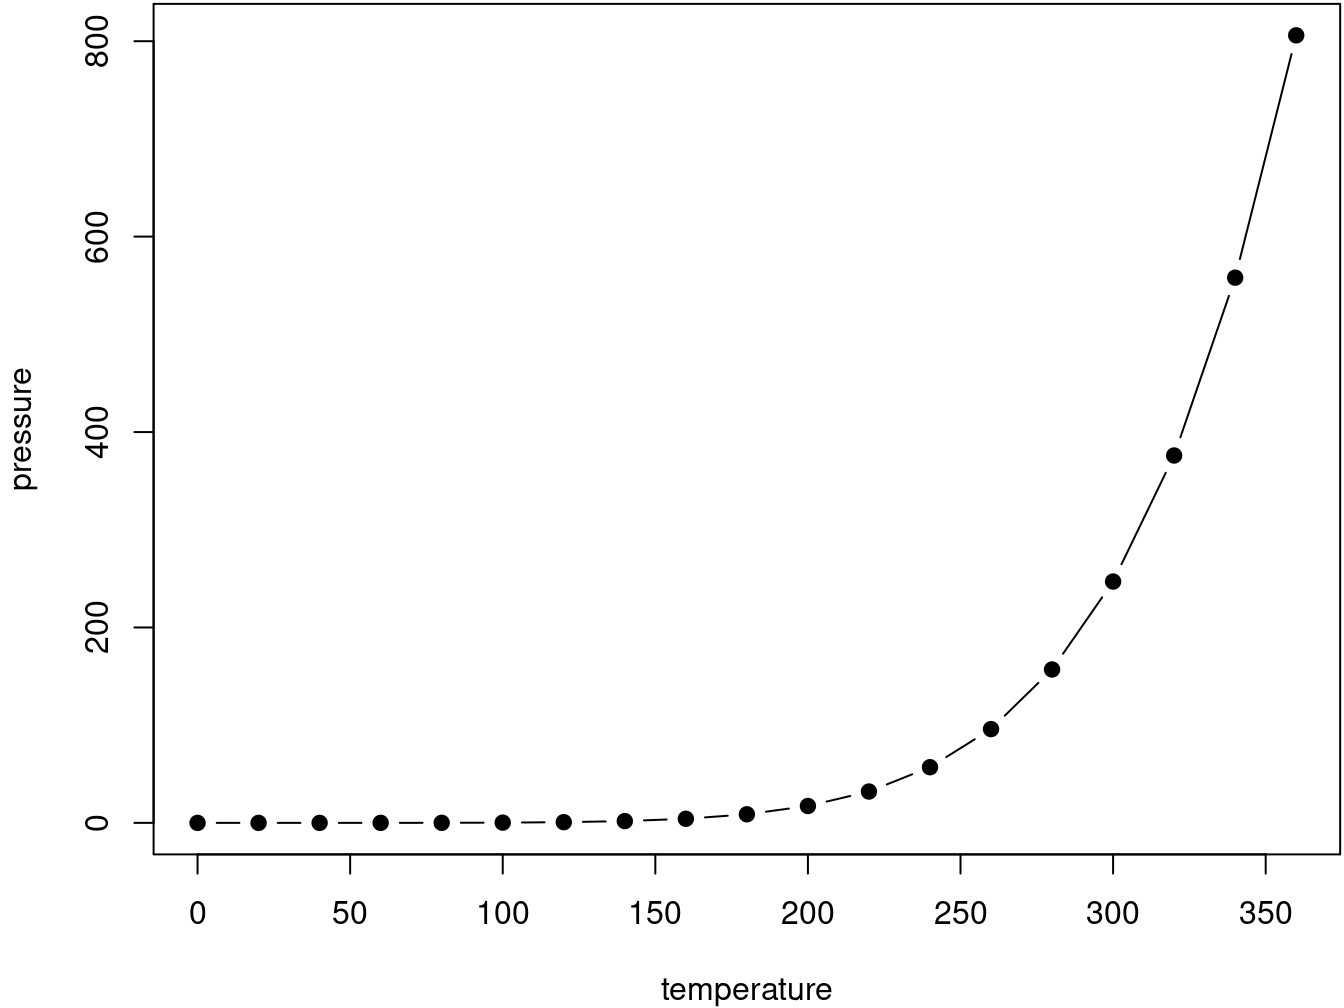
\includegraphics[width=0.8\linewidth]{data-science-practices-1_files/figure-latex/nice-fig-1} 

}

\caption{Here is a nice figure!}\label{fig:nice-fig}
\end{figure}

Reference a figure by its code chunk label with the \texttt{fig:} prefix, e.g., see Figure \ref{fig:nice-fig}. Similarly, you can reference tables generated from \texttt{knitr::kable()}, e.g., see Table \ref{tab:nice-tab}.

\begin{Shaded}
\begin{Highlighting}[]
\NormalTok{knitr}\OperatorTok{::}\KeywordTok{kable}\NormalTok{(}
  \KeywordTok{head}\NormalTok{(iris, }\DecValTok{20}\NormalTok{), }\DataTypeTok{caption =} \StringTok{\textquotesingle{}Here is a nice table!\textquotesingle{}}\NormalTok{,}
  \DataTypeTok{booktabs =} \OtherTok{TRUE}
\NormalTok{)}
\end{Highlighting}
\end{Shaded}

\begin{table}

\caption{\label{tab:nice-tab}Here is a nice table!}
\centering
\begin{tabular}[t]{rrrrl}
\toprule
Sepal.Length & Sepal.Width & Petal.Length & Petal.Width & Species\\
\midrule
5.1 & 3.5 & 1.4 & 0.2 & setosa\\
4.9 & 3.0 & 1.4 & 0.2 & setosa\\
4.7 & 3.2 & 1.3 & 0.2 & setosa\\
4.6 & 3.1 & 1.5 & 0.2 & setosa\\
5.0 & 3.6 & 1.4 & 0.2 & setosa\\
\addlinespace
5.4 & 3.9 & 1.7 & 0.4 & setosa\\
4.6 & 3.4 & 1.4 & 0.3 & setosa\\
5.0 & 3.4 & 1.5 & 0.2 & setosa\\
4.4 & 2.9 & 1.4 & 0.2 & setosa\\
4.9 & 3.1 & 1.5 & 0.1 & setosa\\
\addlinespace
5.4 & 3.7 & 1.5 & 0.2 & setosa\\
4.8 & 3.4 & 1.6 & 0.2 & setosa\\
4.8 & 3.0 & 1.4 & 0.1 & setosa\\
4.3 & 3.0 & 1.1 & 0.1 & setosa\\
5.8 & 4.0 & 1.2 & 0.2 & setosa\\
\addlinespace
5.7 & 4.4 & 1.5 & 0.4 & setosa\\
5.4 & 3.9 & 1.3 & 0.4 & setosa\\
5.1 & 3.5 & 1.4 & 0.3 & setosa\\
5.7 & 3.8 & 1.7 & 0.3 & setosa\\
5.1 & 3.8 & 1.5 & 0.3 & setosa\\
\bottomrule
\end{tabular}
\end{table}

You can write citations, too. For example, we are using the \textbf{bookdown} package \citep{R-bookdown} in this sample book, which was built on top of R Markdown and \textbf{knitr} \citep{xie2015}.

\hypertarget{acknowledgements}{%
\chapter{Acknowledgements}\label{acknowledgements}}

The authors thank all our colleagues for the discussions and experiences about data science that lead to this book. At OUHSC, this includes
\href{https://github.com/adrose}{@adrose},
\href{https://github.com/aggie-dbc}{@aggie-dbc},
\href{https://github.com/ARPeters}{@ARPeters},
\href{https://github.com/Ashley-Jorgensen}{@Ashley-Jorgensen},
\href{https://github.com/athumann}{@athumann},
\href{https://github.com/atreat1}{@atreat1},
\href{https://github.com/caston60}{@caston60},
\href{https://github.com/chanukyalakamsani}{@chanukyalakamsani},
\href{https://github.com/CWilliamsOUHSC}{@CWilliamsOUHSC},
\href{https://github.com/DavidBard}{@DavidBard},
\href{https://github.com/evoss1}{@evoss1},
\href{https://github.com/genevamarshall}{@genevamarshall},
\href{https://github.com/Maleeha}{@Maleeha},
\href{https://github.com/man9472}{@man9472},
\href{https://github.com/rmatkins}{@rmatkins},
\href{https://github.com/sbohora}{@sbohora},
\href{https://github.com/thomasnwilson}{@thomasnwilson},
\href{https://github.com/vimleshbavadiya}{@vimleshbavadiya},
\href{https://github.com/waleboro}{@waleboro},
\href{https://github.com/YuiYamaoka}{@YuiYamaoka},
\href{https://github.com/yutiantang}{@yutiantang}.

Outside the OUHSC, this includes

\href{https://github.com/andkov}{@andkov},
\href{https://github.com/ben519}{@ben519},
\href{https://github.com/cscherrer}{@cscherrer},
\href{https://github.com/cmodzelewski}{@cmodzelewski},
\href{https://github.com/jimquallen}{@jimquallen},
\href{https://github.com/mhunter1}{@mhunter1},
\href{https://github.com/probinso}{@probinso},
\href{https://github.com/russelljonas}{@russelljonas}, and
\href{https://github.com/spopovych}{@spopovych}.

`r if (knitr::is\_html\_output()) '

\hypertarget{references}{%
\chapter{References}\label{references}}

  \bibliography{book.bib,packages.bib}

\end{document}
